\documentclass[12pt,preprint]{aastex}
%\documentclass[12pt]{aastex}

\bibliographystyle{apj}

%#For adding line numbers:
\usepackage{lineno}
\usepackage{lscape}
\linenumbers

%\usepackage{rotating}
\usepackage{amsmath}
\usepackage{graphicx}
\usepackage{color}
\usepackage{url}
\usepackage{subfigure}


% Change the default indent for itemize/enumerate lists
\usepackage{enumitem}
\setlist{leftmargin=2cm}

% Note, hyperref has to come after other packages!
\usepackage{hyperref}
\usepackage{todonotes}

\usepackage{color}

% LaTeX stylings
\usepackage{xspace}

% Instrument
\newcommand{\Fermi}{{\textit{Fermi}}}
\newcommand{\fermi}{\Fermi}
\newcommand{\lat}{LAT\xspace}

% Fermi Tools
\newcommand{\pointlike}{\ensuremath{\mathtt{pointlike}}\xspace}
\newcommand{\gtlike}{\ensuremath{\mathtt{gtlike}}\xspace}
\newcommand{\fits}{\ensuremath{\mathtt{fits}}\xspace}

\newcommand{\ts}{\ensuremath{\text{TS}}\xspace}
\newcommand{\tsext}{\ensuremath{\ts_\text{ext}}\xspace}
\newcommand{\tsvar}{\ensuremath{\ts_\text{var}}\xspace}
\newcommand{\tscut}{\ensuremath{\ts_\text{cutoff}}\xspace}

% Units
\newcommand{\ph}{\text{ph}\xspace}
\newcommand{\erg}{\text{erg}\xspace}
\newcommand{\cm}{\text{cm}\xspace}
\newcommand{\s}{\text{s}\xspace}
\newcommand{\mev}{\text{MeV}\xspace}
\newcommand{\gev}{\text{GeV}\xspace}
\newcommand{\tev}{\text{TeV}\xspace}

\newcommand{\likelihood}{\ensuremath{\mathcal{L}}\xspace}

% Unit
\newcommand{\fitscommand}[1]{\texttt{#1}}


% References
\newcommand{\secref}[1]{\S~\ref{sec:#1}}
\newcommand{\subsecref}[1]{\S~\ref{subsec:#1}}
\newcommand{\tabref}[1]{Table~\ref{tab:#1}}
\newcommand{\figref}[1]{Figure~\ref{fig:#1}}
\newcommand{\eqnref}[1]{Equation~\ref{eqn:#1}}

\newcommand{\seclabel}[1]{\label{sec:#1}}
\newcommand{\subseclabel}[1]{\label{subsec:#1}}
\newcommand{\tablabel}[1]{\label{tab:#1}}
\newcommand{\figlabel}[1]{\label{fig:#1}}
\newcommand{\eqnlabel}[1]{\label{eqn:#1}}


\graphicspath{{./figures/}}

\begin{document}

\title{Fermi Search for Pulsar Wind Nebulae and constraints on the Galactic TeV source population}
%\shorttitle{PWNCAT2}

\keywords{
Catalogs;
Fermi Gamma-ray Space Telescope; 
Gamma rays: observations; 
pulsar wind nebula
}

\author{
Lots of people\ldots
}


\begin{abstract}
  Since its launch, the \emph{Fermi} satellite has firmly identified seven pulsar wind nebulae (PWNe) and a large number of PWNe candidates, all powered by young and energetic pulsars. Furthermore, PWNe are the most populous class of sources detected at TeV energys followed by the unidentified sources (UNID). Using 45 months of \emph{Fermi}--LAT data, we studied the 10 \gev to 316 \gev $gamma$-ray emission around the position of 58 TeV sources that are either associated with PWNe or unidentified. For each source, we derived a $\gamma$--ray flux or a flux upper limit (when the TeV source is not detected at GeV energies by the \emph{Fermi}--LAT).

The wealth of multi-wavelength data available and the new results provided by the \emph{Fermi}--LAT provide an extraordinary opportunity to constrain the origin of the $\gamma$-ray emission of the large sample of UNID and the radiative processes taking place in known PWNe. 

\end{abstract}

%\listoftodos

%\ifdefined\bwfigures
%  Figures are in black and white
%\else
%  Figures are in color
%\fi

\fermititle

\begin{frame}{Overview}
  \begin{itemize}
    \item Category II Paper
    \item Contact Authors: J. Lande, M. Ackermann, S. Funk
    \item Internal Referees: Marianne Lemoine-Goumard and Johann Cohen-Tanugi
    \item Target Journal: ApJ
    \item Currently submitted to internal referees
    \item Feedback welcome
  \end{itemize}
\end{frame}

\begin{frame}{Paper Outline}
  \begin{itemize}
    \item Description of a new method (\texttt{pointlike}) for analyzing extended sources.
    \item Monte Carlo calculation of false detection rate for extended sources.
    \item Calculation of the LAT's detection threshold 
      to spatially extended sources
    \item Presentation of a new search for spatially extended sources:
      \begin{itemize}
        \item Reanalyzing extension of 12 extended sources in 2FGL
        \item Test AGN from 2LAC for extension to validate the analysis
        \item Present 9 extended sources not in 2FGL
      \end{itemize}
  \end{itemize}
\end{frame}



\section{LAT Description and Observations}

Description goes here\ldots


\section{List of candidates}
As a starting point, we used the catalog of TeV sources provided by the university of Chicago\footnotemark[1] to build our list of candidates. This catalog summarizes the information of all sources detected by the TeV experiments. Looking for PWNe candidates which are galactic sources, we selected the sources located within $\pm$5$\degr$ in latitude.

The Galactic center being a complex region to study with \emph{Fermi}--LAT data, due to contamination by the large density of sources and by the diffuse emission, we removed all sources within 5$\degr$ of the Galactic center. Thus, we did not include to our list the three sources HESS~J1745-303, HESS~J1741-302 and G~0.9+0.1 \textbf{citer Lola + autre papier venant sur les SNRs}.

TeV sources associated to SNRs will not be discussed in this analysis. These sources will be included in a forthcoming paper which aims at bringing constraints on all known SNRs using the \emph{Fermi}--LAT data \textbf{(cite the SNR cat)}.

Finally we removed from this analysis the Crab Nebula and Vela-X. Both were already studied in details (\cite{2010ApJ...708.1254A}, \cite{2012ApJ...749...26B}), and the second is the object of a new analysis \textbf{Grondin et al., Forthcoming}. 

The final list of 56 sources studied in this analysis is summarized in Table~\ref{tab:TeV_sources_nom_exp} together with their morphology as seen in TeV. 


%[18:21:24] Joshua Lande mathcal{L}
%[18:21:28] Joshua Lande texttt{gtlike}
%[18:21:32] Joshua Lande text{TS}
%\newcommand{\gtlike}{\ensuremath{\mathtt{gtlike}}\xspace}


\section{Conventions and methods}

\subsection{Modeling of the regions of interest}

Two different tools were used to perform the spatial and spectral analysis: \gtlike \citep{1996ApJ...461..396M} and \pointlike \citep{2011arXiv1101.6072K, 2012arXiv1207.0027L}. These tools fit a source model to the data along with models for the instrumental, extragalactic and Galactic components of the background. We used the version 09--28--00 of the \emph{Fermi} Science Tools.

\pointlike and \gtlike using two different shapes for the region of interest, we used all events contained in a disk of 5$\degr$ centered on the location of the TeV source when fitting the region with \pointlike and we used a $7\degr \times 7\degr$ square included in the previous disk when fitting the region using \gtlike. We tried to keep the two methods as close as possible by using the same conventions (same spatial binning : $\sim 0.06\degr/$bin, same energy binning : 8 energy bins per decade between 10~GeV and 316~GeV, same optimizer : MINUIT \citep{JamesRoos1975}).

In the following analysis, the Galactic diffuse emission was modeled by the standard LAT diffuse emission ring$-$hybrid model \emph{ring\_2yearp7v6\_v0.fits} for all sources. The residual cosmic-ray background and extragalactic radiation are described by a single isotropic component with a spectral shape described by the file \emph{isotrop\_2year\_P76\_clean\_v0.txt}. The models have been released and described by the \emph{Fermi}-LAT Collaboration through the FSSC\footnote{http://fermi.gsfc.nasa.gov/ssc/data/access/lat/BackgroundModels.html}. In the following, we fixed the isotropic diffuse normalization to limit the number of free parameters and reduce the uncertainties on the fitted parameters.

Sources within 10$\degr$ around each source of interest and listed in the hard source list \textbf{(cite the hard source list paper)} were included in our spatial-spectral model. We replaced potential TeV counterparts by a source with the TeV morphology summarized in Table \ref{tab:TeV_sources}. The spectral parameters of sources closer than 2$\degr$ to the source of interest were left free, while the parameters of all other sources were fixed at the hard source list (1FHL) catalog values.

Table \ref{tab:pulsars} summarizes the sources of our list located close to a pulsar detected by the \emph{Fermi}-LAT \textbf{cite 2PC}. The proximity of the pulsar can lead either to the non detection of a faint source hidden by the pulsed emission or to a contamination at low energy if the pulsar is not included. We decided to include in our analysis all the pulsars if they were outside of the TeV template or if they were more than 0.27$\degr$ away from the source of interest. Section \ref{puls_cont} will show the results for the sources close to the pulsars in the case were we added the pulsar in the model and fitted the TeV source.

Due to the longer integration time of our analysis with respect to the 1FHL catalog (45 vs 36 months in the 1FHL), the appearance of additional sources is expected. To prevent contamination from these sources, we looked over all our regions and added to the model all excesses with a significance above 4.0 $\sigma$ which corresponds to a $\text{TS} >$ 25 with 4 degrees of freedom (2 spatial and 2 spectral, see Section~\ref{signi}). The location and spectral parameters of theses sources are described in Table~\ref{tab:newsources}. We fitted their spectra assuming a pure power--law above 10 GeV.

%Thus, we added the sources summarized in Tab. \ref{tab:newsources} to take these excesses into account. We fitted their spectra assuming a pure power--law above 10~GeV.

%In the regions of \emph{TeV~J2019+407, $\gamma$--Cygnii, MGRO~J2031+41, TeV~J2032+4130} the Galactic diffuse emission is taken into account using the models derived in \citet{Cygnus_loop} in which has been performed a precise study of interstellar emission dedicated for this region. We used the files adapted for the P7 V6 IRFs.

\subsection{Analysis of the shape}

Estimation of the position and extension of each PWNe candidates was performed using \pointlike. \pointlike is an alternate binned likelihood technique, optimized for characterizing the extension of a source (unlike \gtlike), that was extensively tested against \gtlike \citep{2011arXiv1101.6072K, 2012arXiv1207.0027L}. To fit an extended source, \pointlike convolves the extended source shape with the PSF (as a function of energy) and uses the MINUIT library \citep{JamesRoos1975} to maximize the likelihood by simultaneously varying the position, extension, and spectrum of the source. \cite{2012arXiv1207.0027L} present more details on the method used and its validation. 

As previously done in \cite{2012arXiv1207.0027L}, we only used radially-symmetric uniform disk shape (defined in Equation \ref{eq:Disk}) to fit the extension of the GeV emission. In the following, we quote the radius to the edge ($\sigma$) as the size of the source.

\begin{equation}\label{eq:Disk}
I_\text{disk}(x,y)=
\begin{cases}
\frac{1}{\pi\sigma^2} & x^2+y^2\le\sigma^2 \\
0                      & x^2+y^2>\sigma^2.
\end{cases}
\end{equation}

\subsection{Spectral analysis}

We performed the spectral analysis of each TeV candidate using \pointlike and \gtlike, the standard likelihood analysis package for LAT data implemented in the Science Tools and distributed by the FSSC. It is a binned maximum-likelihood method \citep{1996ApJ...461..396M} that was extensively validated for spectral analysis and makes fewer approximations in calculating the likelihood than \pointlike. Both methods provided results in agreement with each other, but all spectral parameters quoted in the following were obtained using \gtlike. The spectrum of each source was determined using the best morphological model provided by \pointlike. Due to the narrow energy range which prevents the detection of curved spectra, we fitted all sources assuming a pure power-law of differential flux K and index $\Gamma$ presented in Equation \ref{PL}. 

\begin{equation}
\label{PL}
\frac{dN}{dE}=K \times \left( \frac{E}{E_0} \right)^{\Gamma}
\end{equation}

To minimize the covariance between K and $\Gamma$, we ran the whole analysis twice. In the first iteration, we fitted the source assuming a power-law model depending on the integral flux N and $\Gamma$ shown in Equation \ref{PLFlux}. 

\begin{equation}
\label{PLFlux}
\frac{dN}{dE}=\frac{N\times(\Gamma +1)\times E^{\Gamma}}{E_{max}^{\Gamma+1}-E_{min}^{\Gamma+1}}
\end{equation}

Using the covariance matrix between the parameters of the fit, we derived the pivot energy $E_p$ computed as the energy at which the relative uncertainty on the differential flux K was minimal \citep{2012ApJS..199...31N}. Then, we refitted the spectrum of the source assuming a power-law spectral model (Equation \ref{PL}) with the scale parameter $E_0$ fixed at $E_p$. 

Once the morphological and spectral fit was determined, we derived the photon flux F(10--316~GeV) in photons cm$^{-2}$ s$^{-1}$ and the energy flux G(10--316~GeV) in erg cm$^{-2}$ s$^{-1}$ defined as:

\begin{eqnarray}
F(10-316 \, \rm GeV) = \int_{10 GeV}^{316 GeV} \frac{dN}{dE} dE\\
G(10-316 \, \rm GeV) = \int_{10 GeV}^{316 GeV} E \frac{dN}{dE} dE
\end{eqnarray}


\subsection{Source significance and extension}
\label{signi}

We measured the source significance using a test statistic (\text{TS}) defined as Equation \ref{eq:TS} , where $\mathcal{L}_1$ corresponds to the likelihood obtained by fitting a model of the source of interest and the background model and $\mathcal{L}_0$ corresponds to the likelihood obtained by fitting the background model only. 

\begin{equation}
\label{eq:TS}
\text{TS}=2\times\log (\mathcal{L}_1/\mathcal{L}_0)
\end{equation}

In the following, all \text{TS} values were calculated using \gtlike and the corresponding significance was evaluated from the $\chi^2$ distribution with the corresponding number of degrees of freedom (d.o.f.).

We applied two criteria to decide if a source was significantly detected or not. We selected sources with a $\text{TS}$ above 16 (3.6 $\sigma$ with 2 d.o.f) when assuming the TeV morphology. Then, we applied a second filter on this list of sources by requiring $\text{TS}>16$ at the best GeV shape as well.

To test the extension of each source, following \cite{2012arXiv1207.0027L}, we defined $\text{TS}_{ext}$ as  Equation \ref{eq:Tsext} where $\mathcal{L}_{ext}$ represents the likelihood under an extended source hypothesis (5 d.o.f.) and $\mathcal{L}_{ps}$ represents the likelihood assuming a point source (4 d.o.f.). The condition for a source to be extended is $\text{TS}_{ext} > 16$.

\begin{equation}
\text{TS}_{ext}=2 \times \log({\mathcal{L}_{ext}}/{\mathcal{L}_{ps}})
\label{eq:Tsext}
\end{equation}

We also compared the GeV morphology to the TeV shape. The TeV shape was fixed and we fitted only the spectra as a power-law. To assess the significance of the GeV morphology compared to the TeV shape, we computed $\text{TS}_{GeV/TeV}$ as Equation \ref{eq:Tstevgev} where $\mathcal{L}_{TeV}$ corresponds to the likelihood obtained by fitting the source assuming the TeV shape and $\mathcal{L}_{GeV}$ to the likelihood obtained by fitting the source using the best shape derived using \emph{Fermi}-LAT data.

\begin{equation}
\text{TS}_{GeV/TeV}=2 \times \log({\mathcal{L}_{GeV}}/{\mathcal{L}_{TeV}})
\label{eq:Tstevgev}
\end{equation}

The correspondence between $\text{TS}_{GeV/TeV}$ and the significance is evaluated from a $\chi^2$ distribution with 2 supplementary d.o.f if the best GeV source is a point-like source and 3 supplementary d.o.f if the best GeV source is an extended source. We considered the GeV morphology to be significantly better than the TeV morphology when the likelihood of the fit is better at more than 3$\sigma$ level, which means $\text{TS}_{GeV/TeV} > 12$ for a point-like source in GeV, or $\text{TS}_{GeV/TeV} > 14$ for an extended source (uniform disk) in GeV. All values of $\text{TS}$, $\text{TS}_{ext}$ and $\text{TS}_{GeV/TeV}$ quoted in the following are obtained using \gtlike.

\subsection{Procedure followed}

The 56 regions summarized in Table~\ref{tab:TeV_sources} were all analyzed using the same procedure with both \gtlike and \pointlike:

\begin{enumerate}
\item{We fitted each source assuming its TeV shape summarized in Table~\ref{tab:TeV_sources}. Here, we fixed the position and morphology and fit the spectrum assuming a pure power-law leading the $\text{TS}$ to follow a $\chi^2$ distribution with only 2 d.o.f. 
\begin{itemize}
\item{For sources with significance above 3.6 $\sigma$ ($\text{TS}>$16 with 2 d.o.f.) we applied steps 2 and 3.} 
\item{For sources with $\text{TS}<$ 16 we derived a 99 \% upper limit on the flux assuming the TeV morphology and a power--law index of 2.}
\end{itemize}}
\item{We fitted the source assuming a point source localized with \pointlike as well as the neighbouring sources within 2$\degr$.}
\item{We fitted the source assuming a disk shape derived using \pointlike and compared this hypothesis to the point source hypothesis.}
\end{enumerate}

To take into account the modifications lead by our analysis and have a consistent analysis between all the regions studied, we performed a third iteration where we fixed the shape of the sources further than 2$\degr$ of the source of interest but included in our region to the best morphology found in this analysis (see section \ref{morph_res}). 
%Je n'arrive pas � �tre clair ici. Peut-etre ai-je fait une erreur. Pour que l'analyse soit coh�rente et ne pas avoir une source mod�lis�e d'une sorte dans une r�gion et d'une autre sorte dans une autre r�gion, j'ai retourn� l'analyse en fixant les sources voisines non pas aux morphologies du 1FHL mais aux morphologies que j'ai trouv�. Par exemple la r�gion de 1632 1634 a �t� tourn�e une premi�re fois en ayant 1640 et 1616 aux morphologies inclues dans le 1FHL. Puis j'ai fait retourner la r�gion avec 1640 et 1616 mod�lis� par les templates TeV). 

For the significant sources ($\text{TS}_{TeV}>$16 and $\text{TS}_{GeV}>$16) we derived both the photon and energy fluxes inferred by the fit with the 1 sigma statistical errors, assuming the best morphology. When the source was not significant ($\text{TS}_{TeV}<$16 or $\text{TS}_{GeV}<$16), we derived a 99 \% Confidence Level (C.L.) Bayesian upper limit on the flux using a pure power-law model with an index fixed at 2, assuming the TeV shape. 

\emph{Fermi}-LAT spectral points were obtained by splitting the 10--316 GeV range into 3 logarithmically spaced energy bins. A 99 \% C.L. upper limit is computed when $\text{TS}<$10 using the approach used by \cite{2012ApJS..199...31N}. The errors on the spectral points represent the statistical errors.


%This algorithm was used two times. During the first iteration we used the data selected in a $8\degr\times 8\degr$ square around the TeV position of the source of interest aligned with galactic coordinates. These region are extended enough to allow a reliable fit of the galactic diffuse template normalization \emph{ring\_2yearp7v6\_v0.fits}. In a second iteration we reduced the square to $4\degr\times4\degr$ and we fixed the galactic diffuse normalization to the value derived during the first iteration.\textbf{Develop}

%We launched a second iteration of this analysis with a smaller roi (4$\degr\times$4$\degr$) fixing the spectrum of the galactic background

\subsection{Systematics on the extension}
\label{systext}

Two main systematic uncertainties can affect the extension fit of the sources: uncertainties in our model of the galactic diffuse emission and uncertainties on our knowledge of the LAT PSF.

To estimate the systematics due to the uncertainty in our knowledge of the PSF, we used the pre-flight Monte Carlo representation of the PSF. Indeed, before launch, the LAT PSF was determined by detector simulations which we verified in accelerator beam tests \citep{2009ApJ...697.1071A}. However, in-flight data revealed a discrepancy above 3 GeV in the PSF compared to the angular distribution of photons. To account for this uncertainty, we refit our extended source candidates using the pre-flight  PSF and consider the difference in extension found using the two PSFs as a systematic error on the extension of a source. This procedure was already used by \cite{2012arXiv1207.0027L}.

To estimate the uncertainties on the galactic diffuse emission, we used a GALPROP-based model and considered the various components of the diffuse emission model separately. We then individually fit the normalizations of each of them in our likelihood analysis. These various components are gamma-rays produced by IC emission, gamma-rays produced by interactions of CRs with atomic and ionized interstellar gas, and gamma-rays produced in the interactions of CRs with molecular gas. The model component describing the gamma-ray intensity from interactions with molecular gas is further subdivided into seven ranges of Galactocentric distance. It is not expected that this diffuse model is superior to the standard LAT model obtained through an all-sky fit. However, adding degrees of freedom to the background model can remove likely spurious sources that correlate with features in the Galactic diffuse emission. Therefore, this tests systematics that may be due to imperfect modeling of the diffuse emission in the region. This procedure was also used by \cite{2012arXiv1207.0027L}.

The total systematic error on the extension of a source was obtained by adding the two errors in quadrature.

\subsection{Systematics on the spectral parameters}
\label{syst}

Three main systematic uncertainties can affect the LAT flux estimate for an extended source: uncertainties in the Galactic diffuse background, uncertainties on the effective area and uncertainties on the shape of the source. 

The dominant uncertainty comes from the Galactic diffuse emission and was estimated by using the GALPROP-based model described in Section~\ref{systext}. 

The second systematic was determined by using modified IRFs whose effective areas bracket the nominal ones. These bracketing IRFs are defined by envelopes above and below the nominal energy dependence of the effective area by linearly connecting differences of (10\%, 5\%, 20\%) at log10(E/MeV) of (2, 2.75, 4), respectively.

The imperfect knowledge of the true $\gamma$-ray morphology introduces a last source of error. We derived an estimate of the uncertainty on the shape of the source by using the best model obtained by TeV experiments and compared it to the best extension value obtained in this analysis. We did not compute this component for the sources where the GeV emission is clearly associated to a contamination by the pulsar. 

We combined these various errors in quadrature to obtain our best estimate of the total systematic uncertainty at each energy and propagated through to the fit model parameters.


\subsection{Results}

First, we tested the sources to see if they
were spatially extended. The localization results are in \tabref{localization}.

\begin{deluxetable}{l*{7}c}
\tabletypesize{\scriptsize}
\tablecaption{Localization and extension fitting results
\label{tab:localization}
}
\input{tables/localization.tex}
\tablecomments{\todo[inline]{Put table comments}}
\end{deluxetable}


Next, we performed a spectral analysis over all energy using the best
fit morphology. \tabref{all_energy} shows the results of the all energy
analysis of the off-peak emission for each pulsar.

Next, we fit a powerlaw independently in each energy
bin. \tabref{each_energy} shows the results of the analysis in separate
energy bins of each pulsar.

Finally, we tested sources to see which were
variable. \tabref{cutoff_test} shows the results of the cutoff test for
pulsars with significant low-energy emission.


\begin{deluxetable}{l*{5}c}
\tabletypesize{\scriptsize}
\tablecaption{All Energy spectral fit for the \todo[inline]{How many pulsars?} \lat-detected Pulsars
\label{tab:all_energy}
}
\tablehead{\colhead{PSR} & \colhead{\ts} & \colhead{$F_{0.1-316}$} & \colhead{$G_{0.1-316}$} & \colhead{$\Gamma$} & \colhead{Luminosity}\\ \colhead{ } & \colhead{ } & \colhead{($10^{-9}\ \ph\,\cm^{-2}\,\s^{-1}$)} & \colhead{($10^{-12}\ \erg\,\cm^{-2}\s^{-1}$)} & \colhead{ } & \colhead{($10^{33}\ \erg\,\s^{-1}$)}}
\startdata
J0007+7303 & 84.0 & $53.36 \pm 9.81$ & $20.08 \pm 2.37$ & $2.74 \pm 0.19$ & None \\
J0030+0451 & 14.1 & $<8.22$ & $<10.61$ & \nodata & None \\
J0034$-$0534 & 42.4 & $16.05 \pm 4.75$ & $8.52 \pm 1.65$ & $2.41 \pm 0.19$ & None \\
J0106+4855 & 0.0 & $<6.80$ & $<8.78$ & \nodata & None \\
J0218+4232 & 34.7 & $50.61 \pm 20.56$ & $18.40 \pm 3.35$ & $2.78 \pm 0.48$ & None \\
J0248+6021 & 18.8 & $<13.60$ & $<17.56$ & \nodata & None \\
J0340+4130 & 25.1 & $10.28 \pm 3.62$ & $9.32 \pm 2.46$ & $2.13 \pm 0.15$ & None \\
J0357+3205 & 0.0 & $<2.97$ & $<3.83$ & \nodata & None \\
J0437$-$4715 & 0.0 & $<1.85$ & $<2.39$ & \nodata & None \\
J0534+2200 & 4959.1 & $559.71 \pm 19.47$ & $397.02 \pm 12.21$ & $2.24 \pm 0.02$ & None \\
J0610$-$2100 & 0.0 & $<3.23$ & $<4.17$ & \nodata & None \\
J0613$-$0200 & 0.0 & $<3.37$ & $<4.35$ & \nodata & None \\
J0614$-$3329 & 15.6 & $<15.81$ & $<20.41$ & \nodata & None \\
J0622+3749 & 1.0 & $<7.81$ & $<10.08$ & \nodata & None \\
J0631+1036 & 14.5 & $<13.79$ & $<17.80$ & \nodata & None \\
J0633+0632 & 4.1 & $<10.19$ & $<13.16$ & \nodata & None \\
J0633+1746 & 2842.4 & $882.74 \pm 30.65$ & $579.06 \pm 23.61$ & $2.28 \pm 0.03$ & None \\
J0659+1414 & 0.0 & $<1.77$ & $<2.29$ & \nodata & None \\
J0729$-$1448 & 0.0 & $<4.85$ & $<6.25$ & \nodata & None \\
J0734$-$1559 & 24.5 & $<12.39$ & $<16.00$ & \nodata & None \\
J0742$-$2822 & 4.3 & $<6.84$ & $<8.83$ & \nodata & None \\
J0751+1807 & 8.1 & $<5.70$ & $<7.36$ & \nodata & None \\
J0835$-$4510 & 600.0 & $389.91 \pm 22.62$ & $327.74 \pm 20.41$ & $2.16 \pm 0.03$ & None \\
J0908$-$4913 & 15.1 & $<24.71$ & $<31.89$ & \nodata & None \\
J0940$-$5428 & 0.0 & $<1.73$ & $<2.24$ & \nodata & None \\
J1016$-$5857 & 0.0 & $<12.09$ & $<15.61$ & \nodata & None \\
J1019$-$5749 & 2.4 & $<12.59$ & $<16.25$ & \nodata & None \\
J1023$-$5746 & 273.4 & $399.13 \pm 37.06$ & $472.93 \pm 35.48$ & $2.03 \pm 0.04$ & None \\
J1024$-$0719 & 0.0 & $<2.30$ & $<2.97$ & \nodata & None \\
J1028$-$5819 & 8.0 & $<26.93$ & $<34.77$ & \nodata & None \\
J1044$-$5737 & 0.0 & $<17.76$ & $<22.92$ & \nodata & None \\
J1048$-$5832 & 0.0 & $<16.77$ & $<21.65$ & \nodata & None \\
J1057$-$5226 & 0.8 & $<5.03$ & $<6.49$ & \nodata & None \\
J1105$-$6107 & 11.0 & $<31.71$ & $<40.93$ & \nodata & None \\
J1119$-$6127 & 164.2 & $112.84 \pm 3.58$ & $92.50 \pm 2.17$ & $2.17 \pm 0.01$ & None \\
J1135$-$6055 & 4.2 & $<6.89$ & $<8.89$ & \nodata & None \\
J1231$-$1411 & 0.0 & $<3.21$ & $<4.14$ & \nodata & None \\
J1357$-$6429 & 0.0 & $<5.72$ & $<7.38$ & \nodata & None \\
J1410$-$6132 & 18.4 & $<42.29$ & $<54.59$ & \nodata & None \\
J1413$-$6205 & 0.0 & $<11.99$ & $<15.48$ & \nodata & None \\
J1418$-$6058 & 0.0 & $<34.10$ & $<44.02$ & \nodata & None \\
J1420$-$6048 & 12.1 & $<31.86$ & $<41.13$ & \nodata & None \\
J1429$-$5911 & 0.0 & $<12.66$ & $<16.34$ & \nodata & None \\
J1459$-$6053 & 0.0 & $<9.08$ & $<11.72$ & \nodata & None \\
J1509$-$5850 & 0.0 & $<9.66$ & $<12.47$ & \nodata & None \\
J1513$-$5908 & 122.6 & $19.15 \pm 7.39$ & $51.40 \pm 8.43$ & $1.79 \pm 0.12$ & None \\
J1531$-$5610 & 0.5 & $<3.52$ & $<4.54$ & \nodata & None \\
J1600$-$3053 & 0.0 & $<1.85$ & $<2.39$ & \nodata & None \\
J1614$-$2230 & 0.9 & $<5.93$ & $<7.65$ & \nodata & None \\
J1620$-$4927 & 39.1 & $79.65 \pm 20.62$ & $64.27 \pm 11.41$ & $2.18 \pm 0.10$ & None \\
J1702$-$4128 & 0.0 & $<5.75$ & $<7.42$ & \nodata & None \\
J1709$-$4429 & 69.0 & $181.80 \pm 36.37$ & $90.11 \pm 34.30$ & $2.46 \pm 0.41$ & None \\
J1713+0747 & 0.0 & $<4.79$ & $<6.18$ & \nodata & None \\
J1718$-$3825 & 0.0 & $<14.54$ & $<18.78$ & \nodata & None \\
J1732$-$3131 & 0.0 & $<8.65$ & $<11.16$ & \nodata & None \\
J1741$-$2054 & 0.0 & $<13.38$ & $<17.27$ & \nodata & None \\
J1744$-$1134 & 74.4 & $47.10 \pm 8.73$ & $27.61 \pm 3.67$ & $2.34 \pm 0.08$ & None \\
J1746$-$3239 & 186.8 & $461.05 \pm 37.05$ & $624.30 \pm 40.49$ & $1.98 \pm 0.03$ & None \\
J1747$-$2958 & 74.0 & $260.88 \pm 40.86$ & $512.22 \pm 68.60$ & $1.87 \pm 0.04$ & None \\
J1803$-$2149 & 6.1 & $<27.06$ & $<34.93$ & \nodata & None \\
J1809$-$2332 & 29.0 & $85.89 \pm 68.64$ & $43.14 \pm 9.05$ & $2.45 \pm 0.62$ & None \\
J1813$-$1246 & 53.3 & $191.30 \pm 40.97$ & $83.32 \pm 11.83$ & $2.57 \pm 0.14$ & None \\
J1823$-$3021A & 2.7 & $<5.16$ & $<6.66$ & \nodata & None \\
J1826$-$1256 & 18.4 & $<66.21$ & $<85.47$ & \nodata & None \\
J1836+5925 & 5019.4 & $561.39 \pm 17.71$ & $538.66 \pm 25.37$ & $2.11 \pm 0.02$ & None \\
J1846+0919 & 0.0 & $<3.35$ & $<4.32$ & \nodata & None \\
J1907+0602 & 0.0 & $<7.27$ & $<9.39$ & \nodata & None \\
J1939+2134 & 0.0 & $<4.40$ & $<5.68$ & \nodata & None \\
J1952+3252 & 0.4 & $<7.78$ & $<10.05$ & \nodata & None \\
J1954+2836 & 6.1 & $<18.52$ & $<23.91$ & \nodata & None \\
J1957+5033 & 0.0 & $<2.52$ & $<3.26$ & \nodata & None \\
J1958+2846 & 0.0 & $<7.72$ & $<9.97$ & \nodata & None \\
J1959+2048 & 0.0 & $<4.89$ & $<6.32$ & \nodata & None \\
J2017+0603 & 0.0 & $<2.97$ & $<3.83$ & \nodata & None \\
J2021+3651 & 0.1 & $<7.88$ & $<10.18$ & \nodata & None \\
J2021+4026 & 936.6 & $1196.46 \pm 26.76$ & $824.96 \pm 13.64$ & $2.25 \pm 0.01$ & None \\
J2028+3332 & 0.0 & $<4.57$ & $<5.90$ & \nodata & None \\
J2030+3641 & 0.0 & $<2.89$ & $<3.73$ & \nodata & None \\
J2030+4415 & 3.5 & $<28.40$ & $<36.66$ & \nodata & None \\
J2032+4127 & 91.3 & $192.51 \pm 51.56$ & $425.89 \pm 53.73$ & $1.84 \pm 0.08$ & None \\
J2043+2740 & 0.0 & $<2.58$ & $<3.33$ & \nodata & None \\
J2051$-$0827 & 0.0 & $<1.89$ & $<2.44$ & \nodata & None \\
J2055+2539 & 109.0 & $46.79 \pm 6.38$ & $21.45 \pm 2.28$ & $2.52 \pm 0.08$ & None \\
J2124$-$3358 & 106.5 & $20.21 \pm 3.88$ & $18.48 \pm 3.09$ & $2.13 \pm 0.10$ & None \\
J2139+4716 & 16.8 & $<9.29$ & $<11.99$ & \nodata & None \\
J2214+3000 & 0.0 & $<5.02$ & $<6.48$ & \nodata & None \\
J2238+5903 & 0.0 & $<6.19$ & $<7.99$ & \nodata & None \\
J2240+5832 & 0.0 & $<6.37$ & $<8.22$ & \nodata & None \\
J2302+4442 & 115.0 & $33.65 \pm 5.34$ & $18.69 \pm 2.23$ & $2.38 \pm 0.10$ & None \\
\enddata
\tablecomments{\todo[inline]{Put table comments}}
\end{deluxetable}

\clearpage
\begin{deluxetable}{l*{9}c}
%\tabletypesize{\tiny}
\setlength{\tabcolsep}{0.04in}
\tabletypesize{\scriptsize}
\tablewidth{0pt}
\rotate
\tablecaption{Energy bin spectral fit for the \todo[inline]{How many pulsars?} \lat-detected Pulsars
\label{tab:each_energy}
}
\tablehead{
\colhead{TeV source} & \colhead{$\text{TS (10--31 GeV)}$} & \colhead{F(10--31 GeV)} & \colhead{$\text{TS (31--100 GeV)}$} & \colhead{F(31--100 GeV)} & \colhead{$\text{TS (100--316 GeV)}$} & \colhead{F(100--316 GeV)}\\
\colhead{} &  \colhead{} & \colhead{($10^{-10}$ ph cm$^{-2}$ s$^{-1}$)} & \colhead{} & \colhead{($10^{-11}$ ph cm$^{-2}$ s$^{-1}$)} & \colhead{} & \colhead{($10^{-11}$ ph cm$^{-2}$ s$^{-1}$)}}
\startdata
HESS J1018-589 & 24.7 & 1.3 $\pm$ 0.5 $\pm$ 0.5 & 0.5 & $<$ 5.9 & 5.7 & $<$ 6.2 \\
HESS J1023-575 & 42.8 & 3.7 $\pm$ 0.8 $\pm$ 1.4 & 1.6 & $<$ 9.0 & 18.3 & 1.8 $\pm$ 0.5 $\pm$ 0.9\\
HESS J1119-614 & 17.1 & 1.6 $\pm$ 0.5 $\pm$ 0.5 & 1.0 & $<$ 7.5 & 11.0  & 1.3 $\pm$ 0.6 $\pm$ 0.6\\
HESS J1303-631 & 20.9 & 3.6 $\pm$ 0.9 $\pm$ 1.4 & 26.6 & 17.1 $\pm$ 0.5 $\pm$ 0.6& 7.8 & $<$ 10.7 \\
HESS J1356-645 & 0.2 & $<$ 9.4 & 14.7 & 1.4 $\pm$ 0.7 $\pm$ 0.4 & 10.7 & 6.5 $\pm$ 1.7 $\pm$ 1.7 \\
HESS J1418-609 & 28.7 & 3.7 $\pm$ 0.9 $\pm$ 1.2 & 1.7 & $<$ 10.5 & 0.2 & $<$ 5.4 \\
HESS J1420-607 & 18.1 & 2.4 $\pm$ 0.7 $\pm$ 0.7 & 12.0 & 6.8 $\pm$ 2.6 $\pm$ 3.0 & 12.0 & 4.0 $\pm$ 1.7 $\pm$ 2.1 \\
HESS J1507-622 & 18.2 & 1.4 $\pm$ 0.4 $\pm$ 0.4 & 2.8 & $<$ 7.0 & 0.5 & $<$ 3.9 &\\
HESS J1514-591 & 69.6 & 3.9 $\pm$ 0.7 $\pm$ 1.0 & 65.7 & 15.8 $\pm$ 3.9 $\pm$ 4.8 & 36.8 & 6.7 $\pm$ 2.5 $\pm$ 2.7\\
HESS J1614-518 & 73.4 & 7.9 $\pm$ 1.2 $\pm$ 2.6 & 52.4 & 27.6 $\pm$ 5.9 $\pm$ 11.6 & 27.1 & 9.1 $\pm$ 3.2 $\pm$ 4.6\\
HESS J1616-508 & 46.8 & 6.5 $\pm$ 1.2 $\pm$ 2.0 & 28.4 & 19.9 $\pm$ 5.4 $\pm$ 9.5 & 4.0 & $<$ 10.1 \\
HESS J1632-478 & 71.2 & 10.3 $\pm$ 1.5 $\pm$ 4.2 & 38.1 & 28.2 $\pm$ 6.4 $\pm$ 11.4 & 37.6 & 15.4 $\pm$ 4.4 $\pm$ 6.3 \\
HESS J1634-472 & 15.5 & 3.6 $\pm$ 1.0 $\pm$ 1.9 & 11.7  & 10.8 $\pm$ 3.7 $\pm$ 5.7 & 2.1 & $<$ 8.3 \\
HESS J1640-465 & 20.1 & 3.4 $\pm$ 0.9 $\pm$ 1.5 & 32.2 & 15.1 $\pm$ 4.5 $\pm$ 6.9 & 0 & $<$ 4.5 \\
HESS J1708-443 & 1131.3 & 22.0 $\pm$ 1.5 $\pm$ 3.2 & 22.0 & 5.0 $\pm$ 1.3 $\pm$ 2.0 & 0.0 & $<$ 6.3 \\
HESS J1804-216 & 83.7 & 9.6 $\pm$ 1.4 $\pm$ 2.5 & 37.1 & 24.6 $\pm$ 6.1 $\pm$ 10.7 & 20.8 & 10.4 $\pm$ 3.9 $\pm$ 5.1\\
HESS J1825-137 & 18.2 & 6.4 $\pm$ 1.7 $\pm$ 3.4 & 46.7 & 50.5 $\pm$ 9.4 $\pm$ 20.4 & 19.4 & 11.9 $\pm$ 4.4 $\pm$ 5.5 &\\
HESS J1834-087 & 21.9 & 4.4 $\pm$ 1.6 $\pm$ 1.9 & 7.0 & $<$ 18.7 & 2.5 & $<$ 9.7\\
HESS J1837-069 & 30.6 & 6.9 $\pm$ 1.4 $\pm$ 3.1 & 24.3 & 25.6 $\pm$ 6.7 $\pm$ 10.5 & 28.3 & 15.2 $\pm$ 4.6 $\pm$ 5.9 \\
HESS J1841-055 & 22.8 & 6.4 $\pm$ 1.6 $\pm$ 3.0 & 11.0 & 19.6 $\pm$ 7.1 $\pm$ 5.7 & 22.1 &14.5 $\pm$ 4.5 $\pm$ 7.0 \\
HESS J1848-018 & 16.0 & 5.8 $\pm$ 1.6 $\pm$ 3.1 & 4.2 & $<$ 26.0 & 0.4 & $<$ 10.1\\
HESS J1857+026 & 1.9 & $<$ 2.5 & 12.9 & 13.8 $\pm$ 4.5 $\pm$ 6.8 & 39.3 & 13.0 $\pm$ 4.5 $\pm$ 4.6\\
MGRO J0632+17 & 2144.4 & 27.6 $\pm$ 1.6 $\pm$ 9.8 & 13.0 & 3.0 $\pm$ 1.0 $\pm$ 1.7 & 0 & $<$ 3.8 \\
MGRO J1908+06 & 32.1  & 2.6 $\pm$ 0.5 $\pm$ 1.2 & 0.0  & $<$ 5.0 & 2.8 & 8.6 \\
MGRO J1958+2848 & 18.9 & 1.3 $\pm$ 0.5 $\pm$ 0.4 & 0 & $<$ 3.3 & 0 & $<$3.0\\
MGRO J2019+37 & 100.1 & 3.7 $\pm$ 0.7 $\pm$ 1.5 & 0 & $<$ 3.2 & 2.4 & $<$ 4.9 \\
MGRO J2031+41 & 66.7 & 4.6 $\pm$ 0.8 $\pm$ 1.3 & 5.2 & $<$ 9.4 & 0 & $<$ 3.6\\
MGRO J2228+61 & 108.8 & 2.7 $\pm$ 0.5 $\pm$ 0.5 & 8.0 & $<$ 7.0 & 0 & $<$2.3 \\
VER J0006+727 & 1181.0 & 12.3 $\pm$ 0.9 $\pm$ 2.0 & 38.4 &  3.9 $\pm$ 1.6 $\pm$ 1.6 & 1.5 & $<$ 3.2\\
VER J2016+372 & 25.9 & 1.6 $\pm$ 0.4 $\pm$ 0.5 & 3.4 & $<$ 5.9  & 3.2& $<$ 5.0 \\
\enddata
\tablecomments{\todo[inline]{Put table comments}}
\end{deluxetable}

\begin{deluxetable}{l*{6}c}
\tabletypesize{\scriptsize}
\tablecaption{Spectral fitting of pulsar wind nebula candidates with low energy component
\label{tab:cutoff_test}
}
\tablehead{\colhead{PSR} & \colhead{$\ts_\text{point}$} & \colhead{$\ts_\text{cutoff}$} & \colhead{$F_{0.1-316}$} & \colhead{$G_{0.1-316}$} & \colhead{$\Gamma$} & \colhead{$E_\text{cutoff}$}\\ \colhead{ } & \colhead{ } & \colhead{ } & \colhead{($10^{-9}$\ erg\,cm$^{-2}$\,s$^{-1}$)} & \colhead{($10^{-12}$\ erg\,cm$^{-2}$\,s$^{-1}$)} & \colhead{ } & \colhead{(GeV)}}
\startdata
J0007+7303 & 84.0 & 0.0 & \nodata & \nodata & \nodata & \nodata \\
J0034$-$0534 & 42.4 & 5.5 & \nodata & \nodata & \nodata & \nodata \\
J0218+4232 & 34.7 & 2.8 & \nodata & \nodata & \nodata & \nodata \\
J0340+4130 & 25.1 & 17.2 & $2.38 \pm 1.52$ & $4.95 \pm 1.47$ & $-1.20 \pm 3.36$ & $0.58 \pm 0.66$ \\
J0534+2200 & 4959.1 & 0.0 & \nodata & \nodata & \nodata & \nodata \\
J0633+1746 & 2842.4 & 176.1 & $711.67 \pm 31.00$ & $415.72 \pm 12.92$ & $1.40 \pm 0.10$ & $1.00 \pm 0.12$ \\
J0835$-$4510 & 304.7 & 23.7 & $260.77 \pm 22.71$ & $115.15 \pm 7.65$ & $1.84 \pm 0.17$ & $1.00 \pm 0.30$ \\
J1023$-$5746 & 83.0 & 0.0 & \nodata & \nodata & \nodata & \nodata \\
J1119$-$6127 & 123.2 & 0.0 & \nodata & \nodata & \nodata & \nodata \\
J1513$-$5908 & 122.6 & 0.0 & \nodata & \nodata & \nodata & \nodata \\
J1620$-$4927 & 39.1 & 43.8 & $80.75 \pm 20.97$ & $70.24 \pm 10.35$ & $0.48 \pm 0.39$ & $0.65 \pm 0.16$ \\
J1709$-$4429 & 30.7 & 7.4 & \nodata & \nodata & \nodata & \nodata \\
J1744$-$1134 & 74.4 & 13.7 & \nodata & \nodata & \nodata & \nodata \\
J1746$-$3239 & 47.6 & 33.3 & $64.84 \pm 16.74$ & $39.00 \pm 6.10$ & $0.79 \pm 0.61$ & $0.50 \pm 0.24$ \\
J1747$-$2958 & 30.3 & 12.6 & \nodata & \nodata & \nodata & \nodata \\
J1809$-$2332 & 29.0 & 10.8 & \nodata & \nodata & \nodata & \nodata \\
J1813$-$1246 & 53.3 & 3.4 & \nodata & \nodata & \nodata & \nodata \\
J1836+5925 & 5019.4 & 203.4 & $449.37 \pm 14.27$ & $330.04 \pm 8.76$ & $1.40 \pm 0.03$ & $1.64 \pm 0.06$ \\
J2021+4026 & 920.6 & 138.0 & $949.97 \pm 56.79$ & $586.25 \pm 21.87$ & $1.64 \pm 0.08$ & $1.81 \pm 0.26$ \\
J2032+4127 & 28.5 & 0.0 & \nodata & \nodata & \nodata & \nodata \\
J2055+2539 & 109.0 & 26.3 & $32.23 \pm 2.43$ & $17.45 \pm 1.03$ & $1.51 \pm 0.04$ & $1.00 \pm 0.04$ \\
J2124$-$3358 & 106.5 & 28.7 & $6.61 \pm 2.50$ & $9.86 \pm 1.60$ & $0.06 \pm 0.92$ & $0.87 \pm 0.43$ \\
J2302+4442 & 115.0 & 12.7 & \nodata & \nodata & \nodata & \nodata \\
\enddata
\tablecomments{\todo[inline]{Put table comments}}
\end{deluxetable}




\figref{cutoff_test} shows the cutoff test\ldots

\begin{figure}
  \ifdefined\bwfigures
  \plotone{cutoff_test_bw.eps}
  \else
  \plotone{cutoff_test_color.eps}
  \fi
  \caption{Cutoff test for some pulsars\dots}
  \label{fig:cutoff_test}
\end{figure}


\figref{variability} shows the variability test for each source
candidate. The distribution of \tsvar is plotted in 

\begin{deluxetable}{l*{2}c}
\tabletypesize{\scriptsize}
\tablecaption{Variability test
\label{tab:variability}
}
\tablehead{\colhead{PSR} & \colhead{$\ts_\text{var}$}}
\startdata
J0007+7303 & 29.6 \\
J0030+0451 & 26.6 \\
J0034$-$0534 & 26.0 \\
J0106+4855 & 0.0 \\
J0218+4232 & 77.0 \\
J0248+6021 & 75.4 \\
J0340+4130 & 40.2 \\
J0357+3205 & 0.0 \\
J0437$-$4715 & 0.0 \\
J0534+2200 & 493.7 \\
J0610$-$2100 & 0.0 \\
J0613$-$0200 & 19.6 \\
J0614$-$3329 & 25.6 \\
J0622+3749 & 7.1 \\
J0631+1036 & 30.2 \\
J0633+0632 & 7.8 \\
J0633+1746 & 47.4 \\
J0659+1414 & 0.0 \\
J0729$-$1448 & 0.0 \\
J0734$-$1559 & 29.8 \\
J0742$-$2822 & 27.5 \\
J0751+1807 & 29.6 \\
J0835$-$4510 & 42.7 \\
J0908$-$4913 & 33.1 \\
J0940$-$5428 & 0.0 \\
J1016$-$5857 & 0.0 \\
J1019$-$5749 & 23.6 \\
J1023$-$5746 & 45.5 \\
J1024$-$0719 & 0.0 \\
J1028$-$5819 & 23.6 \\
J1044$-$5737 & 0.0 \\
J1048$-$5832 & 0.0 \\
J1057$-$5226 & 26.9 \\
J1105$-$6107 & 42.9 \\
J1119$-$6127 & 36.9 \\
J1135$-$6055 & 7.2 \\
J1231$-$1411 & 0.0 \\
J1357$-$6429 & 0.0 \\
J1410$-$6132 & 30.3 \\
J1413$-$6205 & 0.0 \\
J1418$-$6058 & 0.0 \\
J1420$-$6048 & 30.5 \\
J1429$-$5911 & 0.0 \\
J1459$-$6053 & 0.0 \\
J1509$-$5850 & 0.0 \\
J1513$-$5908 & 37.5 \\
J1531$-$5610 & 11.0 \\
J1600$-$3053 & 0.0 \\
J1614$-$2230 & 28.1 \\
J1620$-$4927 & 45.5 \\
J1702$-$4128 & 0.0 \\
J1709$-$4429 & 0.0 \\
J1713+0747 & 0.0 \\
J1718$-$3825 & 14.8 \\
J1732$-$3131 & 4.5 \\
J1741$-$2054 & 0.0 \\
J1744$-$1134 & 37.4 \\
J1746$-$3239 & 37.0 \\
J1747$-$2958 & 36.1 \\
J1803$-$2149 & 17.1 \\
J1809$-$2332 & 37.5 \\
J1813$-$1246 & 39.0 \\
J1823$-$3021A & 14.5 \\
J1826$-$1256 & 38.9 \\
J1836+5925 & 30.6 \\
J1846+0919 & 0.0 \\
J1907+0602 & 0.0 \\
J1939+2134 & 5.9 \\
J1952+3252 & 20.1 \\
J1954+2836 & 22.6 \\
J1957+5033 & 0.0 \\
J1958+2846 & 0.0 \\
J1959+2048 & 5.8 \\
J2017+0603 & 0.0 \\
J2021+3651 & 55.7 \\
J2021+4026 & 24.0 \\
J2028+3332 & 0.0 \\
J2030+3641 & 0.0 \\
J2030+4415 & 26.1 \\
J2032+4127 & 25.7 \\
J2043+2740 & 0.0 \\
J2051$-$0827 & 0.0 \\
J2055+2539 & 67.0 \\
J2124$-$3358 & 36.5 \\
J2139+4716 & 40.8 \\
J2214+3000 & 0.0 \\
J2238+5903 & 0.0 \\
J2240+5832 & 0.0 \\
J2302+4442 & 27.9 \\
\enddata
\tablecomments{\todo[inline]{Put table comments}}
\end{deluxetable}

\begin{figure}
  \ifdefined\bwfigures
  \plotone{variability_bw.eps}
  \else
  \plotone{variability_color.eps}
  \fi
  \caption{Distribution of \tsvar for each source candidate. \todo[inline]{Disclaimer about crab not being included}.}
  \label{fig:variability}
\end{figure}


\section{Discussion}
\label{discussion}

%Since \cite{2011ApJ...726...35A} the number of PWNe detected by \emph{Fermi}-LAT increased to X (Crab Nebula, Vela-X, MSH 15-52, HESS J1640, HESS J1825-137, ). This number must be considered with the growing number of PWNe candidates (HESS J1023, HESS J1857, K3 nebula, HESS J1119, HESS J1356, HESS J1303, HESS J1841 and HESS J1848). Table \ref{tab:table_luminosity} shows that these detected sources are located close to young pulsars of characteristic age between 1 and 30 kyr and of spin-down power between $10^{36}$ and $10^{39}$.

%Assuming that the TeV sources were actually associated to the pulsars of Table \ref{tab:table_luminosity}, we used to the pulsars distances to represent on Figure \ref{fig:dotelpwn} the PWN luminosity as a function of the pulsar spin-down power.  

%In this section, we will study the behaviour of the population with physical parameters of the system as the age or the pulsar spin-down power. This analysis follows the work of \cite{2009ApJ...694...12M} where the authors used TeV and X-ray informations.

In this section we investigate the correlations between the pulsar/PWN system parameters (age, spin-down power) and the flux in GeV, TeV and X-ray energy ranges. Tables \ref{tab:table_luminosity} \& \ref{tab:table_luminosity2} summarize the pulsar characteristics and the multi-wavelength informations on each source. To allow the comparison between \cite{2009ApJ...694...12M} and our work, we studied the expected differences between the TeV energy range and the GeV energy range. We assumed that the TeV and the GeV emission coming from these sources were the two sides of the IC emission produced by the same population of electrons and we studied the spectral shape of this IC peak.

Figure \ref{fig:gammagamma} shows the TeV spectral index as a function of the GeV spectral index. This figure perfectly show that sources having a hard index in the GeV energy range ($\Gamma < 2$) have a harder index in the TeV energy range as well, confirming that we may be detecting the two sides of the same $\gamma$-ray peak.

To quantify the expected differences seen in GeV and TeV, we estimated the average energy of the IC peak. For that, we assumed that the $\gamma$-ray energy spectra can be described by a log-normal representation (Equation \ref{logp}) as done in  \cite{2008ApJ...674.1037A}.

\begin{equation}
\label{logp}
\frac{dN}{dE}=N_0 \times \left(\frac{E}{E_0}\right)^{-\left[ \alpha + \beta \times \log\left(\frac{E}{E_b}\right) \right]} 
\end{equation}

We fixed $E_0$ at 300 GeV and $\beta$ at 0.2 and fitted the prefactor $N_0$, the index $\alpha$ and the energy break $E_b$ using our \emph{Fermi}-LAT results and the TeV spectra. Then, we defined the energy of the peak ($E_{peak}$) as the energy at which the energy flux of the modeled peak is maximal. This also corresponds to Equation \ref{pos_epeak}.

\begin{equation}
\label{pos_epeak}
\alpha + \beta \times \log\left(\frac{E}{E_b}\right) = 2.0
\end{equation}

The fit results as well as the peak position are presented in Table \ref{tab:Epeak}. Figure \ref{fig:EpeakETeV} presents the TeV spectral index as a function of the energy of the maximum of the IC peak. This figure highlights a correlation between the TeV spectral index and the peak energy. The TeV index increases with decreasing peak energy except for HESS J1632$-$472. This means that the closer the energy peak is from the GeV energy range, the softer the index will be in the TeV energy range, which is consistent with our log parabola model. The exception of HESS J1632$-$472 could be due to the uncertainties due to the presence of neighbouring sources. As discussed in Section \ref{morph_res}, three sources are detected at lower energies \citep{2012ApJS..199...31N}. These sources are not significantly detected above 10 GeV. It means that these sources can contaminate the low energy of the spectrum derived in this analysis and therefore artificially decrease the fitted energy of the maximum of the IC peak.

Figure \ref{fig:Epeakage} shows the peak energy as a function of the pulsar characteristic age. This Figure presents no obvious correlation between the energy of the peak and the pulsar characteristic age as it would be expected from evolution models and presented in \cite{2012arXiv1202.1455M}. However, it is important to note that this Figure suffers two main biases. First, the characteristic age may not be a good age estimator for the PWN. For instance, MSH 15$-$52 is a known case where two ages are proposed, either the characteristic age of the pulsar 1.7 kyr or an age between 20 and 40 kyr as suggested by the size and general appearance of the SNR \citep{2001AA...374..259G}. Second, our sample is relatively restricted to PWNe with a characteristic age close to 10 kyr, except for MSH 15$-$52 and HESS J1119$-$614. In this context it is not surprising that no correlation is found between $E_{peak}$ and the characteristic age. 

From Table \ref{tab:Epeak} we derived the mean parameters corresponding to our sources of interest : $\bar{\alpha} = 2.1 \pm 0.2$ and $\log_{10}\left(\bar{E_{peak}}\right)= 5.7 \pm 0.6$. Using these parameters we computed the mean expected ratio between the GeV and the TeV fluxes : $\bar{R}=1.9 \pm xx$. Figure \ref{fig:rapportTeV} presents the ratio of the luminosity in the GeV energy range over the luminosity found in the TeV energy range summarized in Table \ref{tab:table_luminosity2}. We represented the mean ratio found between the GeV and TeV energy ranges as a dashed line. This figure shows that no sources are located at more than 2$\sigma$ from this mean ratio except HESS J1804$-$216. \cite{2012ApJ...744...80A} studied the link between the TeV and the GeV emission and concluded that a theory assuming the energy-dependent diffusion of particles accelerated in the SNR is more likely than a PWN scenario. Therefore, the emission is not clearly associated to an IC peak and could have an hadronic origin, which would explain why this source is an outlier.  

As described in \cite{2009ApJ...694...12M}, the $\gamma$-ray and the X-ray luminosities are expected to decrease with time, but the evolution should be different following the age and the pulsar spin-down power. From Table \ref{tab:table_luminosity2} we represent the ratio of the $\gamma$-ray luminosity over the X-ray luminosity as a function of the age and as a function of the pulsar spin-down power. We also represented respectively in solid and dashed line the relations derived in \cite{2009ApJ...694...12M} multiplied by $\bar{R}$ for the whole sample of sources and for the sources clearly identify to PWNe.

This figure show two correlations : one between the fluxes ratio and the spin-down power and the other between the same flux ratio and the characteristic age. These correlations are expected since the magnetic field depends on these two parameters. However, for each correlation, a sample of four upper limits consistent with fluxes measured at TeV energies are well below the correlation relations derived by \cite{2009ApJ...694...12M}. The overall agreement with the relations proposed by \cite{2009ApJ...694...12M} is relatively good but it can already be predicted that the GeV points will have a larger dispersion once these sources will be detected. 

It seems clear from these figures that \emph{Fermi}-LAT mainly detect young and middle-aged PWNe (1-30 kyr) around energetic pulsars with a spin-down power between 10$^{36}$ and 10$^{37}$ erg s$^{-1}$. Figure \ref{fig:dotelpwn} shows the $\gamma$-ray luminosity of the PWN as a function of the pulsar spin-down power assuming the distances summarized in Table \ref{tab:table_luminosity}. The solid, dashed and dot dashed lines respectively show the lines where the luminosity corresponds to 100\%, 10\% and 1\% of the spin-down power. Full and hollow markers respectively represent sources for which the TeV emission is clearly associated to a PWNe and sources for which the association is less clear. Sources with a pulsar-like spectrum are represented in green pentagons. For all sources in Table \ref{tab:pulsars} the pulsar are included in the models. Among the detected sources, eight show a $\gamma$-ray efficiency below 1\% and five are consistent within uncertainties with  an efficiency between 1 an 10 \%. HESS J1303$-$631 is also consistent with an efficiency of 100\% assuming a distance of 15 kpc. This can be due to the large uncertainty on the distance measured which can lead to a factor 3 between the estimated distance and the true distance and by the contamination by Kes 17 as discussed in Section \ref{morph_res}. Six upper limits on the luminosity of TeV sources clearly associated to PWNe are well below an efficiency of 1\%.

\section{Conclusion}

45 months of \emph{Fermi}-LAT observations have been used to look for counterparts to the TeV sources potentially associated to PWNe. Among the 58 sources studied, 31 have been detected. Among these 31, 23 were also detected in \cite{1FHL} and 15 in \cite{2012PhRvD..85h3008N}. Interestingly five new sources are detected in our analysis (HESS J1119$-$614, HESS J1303$-$631, HESS J1356$-$645, HESS J1841$-055$ and HESS J1848$-$018). We analyzed the morphology of the 31 sources detected and found that for 19 of them the GeV shape did not significantly improve the fit in comparison to the TeV shape. For five sources, we found a significant extension larger than the TeV morphology. Six sources are well fitted by a point-like source; all of them have a high index and are probably associated to pulsars emitting above 10 GeV.

Since \cite{2011ApJ...726...35A} the number of PWNe detected by \emph{Fermi}-LAT increased to 5 (Crab Nebula, Vela-X, MSH 15$-$52, HESS J1640$-$465, HESS J1825$-$137 ). This number must be considered with the growing number of PWNe candidates (HESS J1023$-$577, HESS J1119$-$614, HESS J1303$-$631, HESS J1356$-$645, HESS J1420$-$607, HESS J1841$-$055, HESS J1848$-$018 and HESS J1857+026). These PWNe and PWNe candidates are powered by young (between 1 and 30 kyr) and powerfull pulsars (spin down power between 10$^{36}$ and 10$^{39}$ erg s$^{-1}$ with an efficiency below 10\%.


The \textit{Fermi} LAT Collaboration acknowledges generous ongoing support
from a number of agencies and institutes that have supported both the
development and the operation of the LAT as well as scientific data analysis.
These include the National Aeronautics and Space Administration and the
Department of Energy in the United States, the Commissariat \`a l'Energie Atomique
and the Centre National de la Recherche Scientifique / Institut National de Physique
Nucl\'eaire et de Physique des Particules in France, the Agenzia Spaziale Italiana
and the Istituto Nazionale di Fisica Nucleare in Italy, the Ministry of Education,
Culture, Sports, Science and Technology (MEXT), High Energy Accelerator Research
Organization (KEK) and Japan Aerospace Exploration Agency (JAXA) in Japan, and
the K.~A.~Wallenberg Foundation, the Swedish Research Council and the
Swedish National Space Board in Sweden.

Additional support for science analysis during the operations phase is
gratefully acknowledged from the Istituto Nazionale di Astrofisica in
Italy and the Centre National d'\'Etudes Spatiales in France.

This research has made use of pywcsgrid2, an open-source plotting package for Python6\footnote{http://leejjoon.github.com/pywcsgrid2/}. The authors acknowledge the use of HEALPix\footnote{\url{http://healpix.jpl.nasa.gov/}} \citep{2005ApJ...622..759G}.

The authors acknowledge the use of the TeV catalog website\footnote{http://tevcat.uchicago.edu/} provided by the university of Chicago.

The authors acknowledge the use of the \emph{Australia Telescope National Facility} pulsar catalog\footnote{http://www.atnf.csiro.au/people/pulsar/psrcat/}.

\clearpage
\newpage
\bibliographystyle{plain}
\bibliography{tevcat}
\nocite{*} %Permet d'afficher toute la bibliographie

\begin{deluxetable}{l*{5}l}
\tabletypesize{\scriptsize}
\tablecaption{List of TeV sources analyzed
\label{tab:TeV_sources}}
\tablehead{\colhead{TeV source} & \colhead{Type} & \colhead{(l,b) ($\degr$)} & \colhead{TeV morphology} & \colhead{Reference}}
\startdata
HESS J1018-589 & UNID &(284.23,-1.72) & pointsource& \citep{2012arXiv1203.3215H} \\
HESS J1023-577 & Massive Star Cluster &(284.22,-0.40) &gaussian(0.18)& \citep{2011AA...525A..46H}\\
HESS J1026-582 & PWN &(284.80,-0.52) &gaussian(0.14)& \citep{2011AA...525A..46H} \\
HESS J1119-614 & PWN &(292.10,-0.49) &gaussian(0.05)& \footnote{http://cxc.harvard.edu/cdo/snr09/pres/DjannatiAtai\_Arache\_v2.pdf}\\
HESS J1303-631 & PWN &(304.24,-0.36) &gaussian(0.16)& \citep{2005AA...439.1013A}\\
HESS J1356-645 & PWN &(309.81,-2.49) &gaussian(0.20)& \citep{2011AA...533A.103H}\\
HESS J1418-609 & PWN &(313.25,0.15) &Ell. gaussian(0.08,0.06)&\citep{2006AA...456..245A}\\
HESS J1420-607 & PWN &(313.56,0.27) &gaussian(0.06)& \citep{2006AA...456..245A}\\
HESS J1427-608 & UNID &(314.41,-0.14) &Ell. gaussian(0.04,0.08)& \citep{2008AA...477..353A}\\
HESS J1458-608 & PWN & (317.75, -1.7) & gaussian(0.17) & \citep{2012arXiv1205.0719D}\\
HESS J1503-582 & UNID &(319.62,0.29) &gaussian(0.26)& \citep{2008AIPC.1085..281R}\\
HESS J1507-622 & UNID &(317.95,-3.49) &gaussian(0.15)& \citep{2011AA...525A..45H}\\
HESS J1514-591 & PWN &(320.33,-1.19) & Ell. gaussian(0.11,0.04)& \citep{2005AA...435L..17A}\\
HESS J1554-550 & PWN &(327.16,-1.07) & pointsource & \citep{2012arXiv1201.0481A}\\
HESS J1614-518 & massive star cluster &(331.52,-0.58) &Ell. gaussian(0.23,0.15)& \citep{2006ApJ...636..777A}\\
HESS J1616-508 & PWN &(332.39,-0.14) &gaussian(0.14)& \citep{2006ApJ...636..777A}\\
HESS J1626-490 & UNID &(334.77,0.05) &Ell. gaussian(0.07,0.10)& \citep{2008AA...477..353A}\\
HESS J1632-478 & PWN &(336.38,0.19) &Ell. gaussian(0.21,0.06)&\citep{2006ApJ...636..777A}\\
HESS J1634-472 & UNID &(337.11,0.22) &gaussian(0.11)&\citep{2006ApJ...636..777A}\\
HESS J1640-465 & PWN &(338.32,-0.02) &gaussian(0.04)&\citep{2006ApJ...636..777A}\\
HESS J1646-458 & Massive Star Cluster & (339.57, -0.02) & gaussian(0.35) & \citep{2012AA...537A.114A}\\
HESS J1646-458 B & Massive Star Cluster & (339.01, -0.79) & gaussian(0.25) & \citep{2012AA...537A.114A}\\
HESS J1702-420 & UNID &(344.30,-0.18) &Ell. gaussian(0.30,0.15)&\citep{2006ApJ...636..777A}\\
HESS J1708-443 & PWN &(343.06,-2.38) &gaussian(0.29)& \citep{2011AA...528A.143H}\\
HESS J1718-385 & PWN &(348.83,-0.49) &Ell. gaussian(0.15,0.07)& \citep{2007AA...472..489A}\\
HESS J1729-345 & UNID &(353.44,-0.13) &gaussian(0.14)& \citep{2011AA...531A..81H}\\
HESS J1804-216 & UNID &(8.40,-0.03) &Ell. gaussian(0.16,0.27)& \citep{2006ApJ...636..777A} \\
HESS J1809-193 & PWN &(11.18,-0.09) &Ell. gaussian(0.53,0.25)&\citep{2007AA...472..489A}\\
HESS J1813-178 & PWN &(12.81,-0.03) &gaussian(0.04)& \citep{2006ApJ...636..777A}\\
HESS J1818-154 & PWN &(15.41,0.17) &gaussian(0.14)& \citep{2011arXiv1112.2901H} \\
HESS J1825-137 & PWN &(17.71,-0.70) &Ell. gaussian(0.13,0.12)&\citep{2006AA...460..365A}\\
HESS J1831-098 & PWN &(21.85,-0.11) &gaussian(0.15)& \citep{2011arXiv1110.6837S}\\
HESS J1833-105 & PWN &(21.51,-0.88) & pointsource& \citep{2008ICRC....2..823D}\\
HESS J1834-087 & UNID &(23.24,-0.31) &gaussian(0.09)& \citep{2006ApJ...636..777A}\\
HESS J1837-069 & UNID &(25.18,-0.12) &Ell. gaussian(0.12,0.05)&\citep{2006ApJ...636..777A}\\
HESS J1841-055 & UNID &(26.80,-0.20) &Ell. gaussian(0.41,0.25)& \citep{2008AA...477..353A}\\
HESS J1843-033 & UNID &(29.30,0.51) & pointsource& \citep{2008ICRC....2..579H}\\
HESS J1846-029 & PWN &(29.70,-0.24) & pointsource& \citep{2008ICRC....2..823D}\\
HESS J1848-018 & Massive Star Cluster &(31.00,-0.16) &gaussian(0.32)& \citep{2008AIPC.1085..372C}\\
HESS J1849-000 & PWN &(32.64,0.53) & pointsource& \citep{2008AIPC.1085..312T}\\
HESS J1857+026 & UNID &(35.96,-0.06) &Ell. gaussian(0.11,0.08)&\citep{2008AA...477..353A}\\
HESS J1858+020 & UNID &(35.58,-0.58) &Ell. gaussian(0.08,0.02)&\citep{2008AA...477..353A}\\
HESS J1912+101 & PWN &(44.39,-0.07) &gaussian(0.26)& \citep{2008AA...484..435A}\\
MGRO J0631+105 & PWN &(201.30,0.51) & pointsource & \citep{2009ApJ...700L.127A}\\
MGRO J0632+17 & PWN &(195.34,3.78) &gaussian(1.30)& \citep{2009ApJ...700L.127A} \\
MGRO J1844-035 & UNID &(28.91,-0.02) & pointsource& \citep{2009ApJ...700L.127A}\\
MGRO J1900+039 & UNID &(37.42,-0.11) & pointsource& \citep{2009ApJ...700L.127A}\\
MGRO J1908+06 & UNID &(40.39,-0.79) &gaussian(0.34)& \citep{2009AA...499..723A}\\
MGRO J1958+2848 & PWN &(65.85,-0.23) & pointsource& \citep{2009ApJ...700L.127A}\\
MGRO J2019+37 & PWN &(75.00,0.39) &gaussian(0.55)& \citep{2007ApJ...664L..91A}\\
MGRO J2031+41 A& UNID &(79.53,0.64) &gaussian(1.50)&\citep{2007ApJ...664L..91A}\\
MGRO J2031+41 B& UNID &(80.25,1.07) &gaussian(0.10)& \citep{2012ApJ...745L..22B}\\
MGRO J2228+611 & PWN &(106.57,2.91) & pointsource& \citep{2009ApJ...700L.127A}\\
VER J0006+727 & PWN &(119.58,10.20) & pointsource& \citep{2011arXiv1111.2591M}\\
VER J1930+188 & PWN &(54.10,0.26) & pointsource& \citep{2010ApJ...719L..69A} \\
VER J1959+208 & PSR &(59.20,-4.70) & pointsource& \citep{2003ApJ...583..853H}\\
VER J2016+372 & UNID &(74.94,1.15) & pointsource& \citep{2011arXiv1110.4656A}\\
W49A & Star Forming Region &(43.27,-0.00) & pointsource& \citep{2011arXiv1104.5003B}\\

%Vela Region & UNID &(263.23,-2.92) & pointsource& \\
\enddata
%\\
%a : P72Y0963 is associated with the pulsar emission of PSR~J0633+1746 located inside of the TeV template use for Geminga


%j'en suis la

\tablecomments{The first two columns list the TeV source names and types as defined in the TeV catalog provided by the university of Chicago: PWN for Pulsar Wind Nebula, PSR for Pulsars, UNID for Unidentified sources, Massive Star Cluster and Star Forming Regions. The 3$^{rd}$ column reports the Galactic coordinates for each source. The 4$^{th}$ column presents the shape that best describes the source at TeV energies, together with a reference in the  5$^{th}$ column.}

\end{deluxetable}


\clearpage
\begin{deluxetable}{llllc}
\tabletypesize{\scriptsize}
\tablecaption{List of sources with a pulsar within 0.5$\degr$
\label{tab:pulsars}}
\tablehead{\colhead{Source name} & \colhead{Pulsar Name} & \colhead{distance ($\degr$)} & \colhead{pulsar 2FGL name} & \colhead{Included in the model}}
\startdata
HESS J1018-589 & PSR J1016-5857 & 0.22 & 2FGL J1016.5-5858 & N \tablenotemark{a}\\
HESS J1023-577 & PSR J1023-5746 & 0.05 & 2FGL J1022.7-5741 & N \tablenotemark{b}\\
HESS J1026-5819 & PSR J1028-5819 & 0.27 & 2FGL J1028.5-5819 & Y\\
HESS J1119-614 & PSR J1119-6127 & 0.07 & 2FGL J1118.8-6128 & N \tablenotemark{a}\\
HESS J1356-645 & PSR J1357-6429 & 0.12 & 2FGL J1356.0-6436 & N \tablenotemark{a}\\
HESS J1418-609 & PSR J1418-6058 & 0.05 & 2FGL J1418.7-6058 & N \tablenotemark{b}\\
HESS J1420-607 & PSR J1420-6048 & 0.05 & 2FGL J1420.1-6047 & N \tablenotemark{b}\\
HESS J1458-608 & PSR J1459-6053 & 0.17 & 2FGL J1459.4-6054 & N \tablenotemark{a}\\
HESS J1514-591 & PSR J1513-5908 & 0.03 & - & N \tablenotemark{b}\\
HESS J1702-420 & PSR J1702-4128 & 0.53 & -- & N \tablenotemark{c}\\
HESS J1708-443 & PSR J1709-4429 & 0.25 & 2FGL J1709.7-4429 & N \tablenotemark{b}\\
HESS J1718-385 & PSR J1718-3825 & 0.13 & 2FGL J1718.3-3827 & N  \tablenotemark{a}\\
HESS J1804-216 & PSR J1803-2149 & 0.27 & 2FGL J1803.3-2148 & N \tablenotemark{b}\\
HESS J1833-105 & PSR J1833-1034 & 0.01 & 2FGL J1833.6-1032 & N  \tablenotemark{a}\\
MGRO J0631+105 & PSR J0631+1036 & 0.10 & 2FGL J0631.5+ 1035 & N  \tablenotemark{a}\\
MGRO J0632+17 & PSR J0633+1746 & 0.00 & 2FGL J0633.9+1746 & N  \tablenotemark{a}\\
MGRO J1908+06 & PSR J1907+0602 & 0.23 & 2FGL J1907.9+0602 & N  \tablenotemark{a}\\
MGRO J1958+2848 & PSR J1958+2846 & 0.12 & 2FGL J1958.6+2845 & N  \tablenotemark{a}\\
MGRO J2019+37 & PSR J2021+3651 & 0.36 & 2FGL J2021.0+3651 & N \tablenotemark{b}\\
MGRO J2228+61 & PSR J2229+6114 & 0.09 & 2FGL J2229+6114 & N  \tablenotemark{a}\\
VER J0006+727 & PSR J0007+7303 & 0.26 & 2FGL J0007.0+7303 & N  \tablenotemark{a}\\
\enddata\\
\begin{flushleft}
a- The distance between the pulsar and the source is lower than 0.27$\degr$.\\
b- The pulsar is located inside the edge of the TeV shape.\\
c- No significant excess above 10 GeV at the position of the pulsar.\\
\end{flushleft}
\tablecomments{ $_{ }$List of sources having a known $\gamma$-ray pulsar within 0.5$\degr$. The two first columns list the TeV source and the pulsar name. The third column gives the distance between the TeV source and the GeV pulsar. The pulsar position comes from \cite{2PC}. In the fourth colum Y means that we added the pulsar to the model and N that we didn't added it.}

\end{deluxetable}

\clearpage
\tabletypesize{\scriptsize}
\begin{deluxetable}{l*{5}l}
\tablewidth{0pt}
\tablecaption{Locations and spectral parameters of additional background sources above 10 GeV 
\label{tab:newsources}}
\tablehead{\colhead{Source name} & \colhead{Galactic coordinates ($\degr$)} & \colhead{$\text{TS}$} & \colhead{Prefactor} & \colhead{Index}}
\startdata
2FGL J1504.5--6121 & (311.81,0.30) & 30.7 & ( 1.2 $\pm$ 0.4 ) $\times 10^{-15}$ & 1.8 $\pm$ 0.3 \\
2FGL J1836.8--0623c & (25.41,0.42) & 25.1 & ( 9.4 $\pm$ 1.9 ) $\times 10^{-16}$ & 2.0 $\pm$ 0.4 \\
2FGL J1823.1--1338c & (17.51,-0.12) & 30.4 & (4.9 $\pm$ 0.5) $\times 10^{-15}$  & 2.9 $\pm$ 0.7\\
PSR J1838--0536 & (26.28,0.62) & 16.1 & (5.0 $\pm$ 1.8) $\times 10^{-17}$ & 4.1 $\pm$ 1.0 \\
Background Source 1 & (333.59,-0.31) & 29 & (6.5 $\pm$ 2.5) $\times 10^{-17}$ & 4.3 $\pm$ 0.9\\
Background Source 2 & (336.96, -0.07) & 25.0 & (1.2 $\pm$ 0.4) $\times 10^{-15}$ & 1.9 $\pm$ 0.4\\
Background Source 3 & (339.37,-1.18) & 29.9 & (1.3 $\pm$ 0.4) $\times 10^{-15}$ & 1.5 $\pm$ 0.3\\
\enddata

\tablecomments{The first two columns describe the source names and their corresponding Galactic coordinates. The test statistic (TS) for the source significance is provided in the 3$^{rd}$ column. The spectral results are presented in columns 4 and 5 for a power-law model (Equation~\ref{PL}) with a scale parameter $E_0 = 56234$ MeV which corresponds to the middle of the 10--316 GeV interval in log scale. PSR~J1838$-$0536 has been added to help the morphology fit of HESS~J1841$-$055 which is a diffuse source. The spectral fit is consistent with the pulsar component (index of$\sim$ 5).}

\end{deluxetable}
\normalsize
\noindent

\clearpage
\tabletypesize{\scriptsize}
\begin{deluxetable}{l*{7}l}
\tablewidth{0pt}
\tablecaption{Morphological results for LAT-detected TeV sources above 10 GeV
\label{tab:Morphology_results}}
\tablehead{\colhead{TeV source} & \colhead{$\text{TS}_{TeV}$} & \colhead{$\text{TS}_{GeV}$} & \colhead{$\text{TS}_{ext}$} & \colhead{$\text{TS}_{GeV/TeV}$} & \colhead{Significance}  & \colhead{Morphology}}
\startdata
HESS J1018-589 & 29.1 & 29.1 & 0 & 0 & 0 & TeV\\
HESS J1023-575 & 52.0 & 49.4 & 1.5 & - & - & TeV\\
HESS J1119-614 & 27.3 & 27.3 & 12.2 & 0 & 0 & TeV \\
HESS J1303-631 & 37.2 & 52.5 & 24.9 & 15.3 & 3.1 & Disk\\
HESS J1356-645 & 25.8 & 28.8 & 2.5 & 3.0 & 1.2 & TeV\\
HESS J1418-609 & 30.4 & 30.9 & 0.1 & - & - & TeV\\
HESS J1420-607 & 41 & 41.2 & 1.8 & - & - & TeV\\
HESS J1507-622 & 20.9 & 22.1 & 7.2 & - & - & TeV\\
HESS J1514-591 & 169.5 & 147.3 & 10.4 & - & - & TeV\\
HESS J1614-518 & 119.6 & 146.3 & 59.6 & 26.7 & 4.5 & Disk\\
HESS J1616-508 & 76.2 & 79.6 & 19.9 & 3.4 & 1.0 & TeV\\
HESS J1632-478 & 120.8 & 143 & 52.4 & 22.2 & 4.3 & Disk\\
HESS J1634-472 & 28.7 & 29.6 & 5.2 & 0.9 & 0.5 & TeV\\
HESS J1640-465 & 49 & 52.9 & 0 & 3.9 & 1.5 & TeV\\
HESS J1708-443 & 721.8 & 1153.3 & 0 & 431.5 & & point--like\\
HESS J1804-216 & 131 & 137.8 & 41.1 & 6.8 & 1.8 & TeV\\
HESS J1825-137 & 55.7 & 78.1 & 27.9 & 22.4 & 4.0 & Disk\\
HESS J1834-087 & 31 & 28.7 & 2.6 & - & - & TeV\\
HESS J1837-069 & 74 & 106.7 & 45.8 & 32.7 & 5.1 & Disk\\
HESS J1841-055 & 52 & 65 & 38.3 & 13.0 & 2.8 & TeV\\
HESS J1848-018 & 18.7 & 18.6 & 0 & - & - & TeV\\
HESS J1857+026 & 52.5 & 53.1 & 12.1 & - & - & TeV\\
MGRO J0632+17 & 698.8 & 2056.3 & 2.5 & 1357.5 & &point--like\\
MGRO J1908+06 & 16.4 & 37.2 & 0.2 & 20.8 & 4.2 & point--like\\
MGRO J1958+2848 & 20.8 & 23.5 & 0.2 & 2.7 & 1.1 & TeV \\
MGRO J2019+37 & 31.1 & 98.5 & 0 & 61.3 & 8.0 & point--like\\
MGRO J2031+41 & 72.1 & 66.4 & 2.9 & - & - & TeV\\
MGRO J2228+61 & 94.5 & 114 & 0 & 19.5 & 4.0 & point--like\\
VER J0006+727 & 654.5 & 1205.6 & 1.3 & 551.1 &  & point--like\\
VER J2016+372 & 31.4 & 32.9 & 0.3 & 1.5 & 0.7 & TeV\\
\enddata

\tablecomments{Results of the morphological analysis for all LAT-detected TeV sources. The fits assumed either the TeV template defined in Table~\ref{tab:TeV_sources}, a point-source model or a uniform disk model (see Equation~\ref{eq:Disk}). The definition of $\text{TS}_{TeV}$, $\text{TS}_{GeV}$, $\text{TS}_{ext}$ and $\text{TS}_{GeV/TeV}$ is reported in Section~\ref{signi}.
The significance of the extension is measured using the $\text{TS}_{ext}$ criterium defined in Section~\ref{signi}.}

\end{deluxetable}
\normalsize
\noindent

\clearpage
\tabletypesize{\scriptsize}
\begin{deluxetable}{l*{5}l}
\tablewidth{0pt}
\tablecaption{Morphological results for LAT-detected TeV sources for which $\text{TS}_{GeV}$ is significantly better than $\text{TS}_{TeV}$ above 10 GeV
\label{tab:GeVmorph}}
\tablehead{\colhead{TeV source} & \colhead{Morphology} & \colhead{$\text{TS}_{ext}$} & \colhead{(l,b) $\degr$}  & \colhead{extension($\degr$)}}
\startdata
HESS J1303-631 & Disk & 24.9 & (304.44, -0.18) & 0.50 $\pm$ 0.05$_{stat}$ \\
HESS J1614-518 & Disk & 59.8 & (331.66, -0.66) & 0.42 $\pm$ 0.06$_{stat}$\\
HESS J1632-478 & Disk & 52.4 & (336.38, 0.19)& 0.45 $\pm$ 0.04$_{stat}$\\
HESS J1708-443 & point--like & 0 & (343.11,-2.70) & -\\
HESS J1825-137 & Disk & 27.9 & (17.56,-0.47) & 0.65 $\pm$ 0.04$_{stat}$\\
HESS J1837-069 & Disk & 45.8 & (25.08,-0.13) & 0.32 $\pm$ 0.05$_{stat}$\\
MGRO J0632+17 & point--like & 2.5 & (195.13, 4.27) &-\\
MGRO J1908+06 & point--like & 0.2 & (40.39, -0.79) & -\\
MGRO J2019+37 & point--like & 0 & (75.27, 0.14) & - \\
MGRO J2228+61 & point--like & 0 & (106.67, 2.93) & - \\
VER J0006+727 & point--like & 1.3 & (119.69, 10.47) &-\\
\enddata


\tablecomments{Results of the morphological analysis for LAT-detected TeV sources better described using the shape fitted at GeV energies. The fits assumed either a point-source model or a uniform disk model (see Equation~\ref{eq:Disk}) whose centroid and extension are provided in columns 4 and 5 respectively. The significance of the extension is measured using the $\text{TS}_{ext}$ criterium defined in Section~\ref{signi}.}

\end{deluxetable}
\normalsize
\noindent

\clearpage
\tabletypesize{\scriptsize}
\begin{deluxetable}{l*{5}l}
\tablewidth{0pt}
\tablecaption{Spectral fitting results for LAT-detected TeV sources above 10 GeV 
\label{tab:det_sources}}
\tablehead{
\colhead{TeV source} & \colhead{$\text{TS}$} & \colhead{F(10--316 GeV)} & \colhead{E(10--316 GeV)} & \colhead{$\Gamma$}\\
\colhead{} & \colhead{} &\colhead{($10^{-10}$ ph cm$^{-2}$ s$^{-1}$)} &\colhead{($10^{-12}$ erg cm$^{-2}$ s$^{-1}$)} &\colhead{}}
\startdata
HESS J1018-589 &$29.1$ & $1.7 \pm 0.5_{stat} \pm 0.6_{syst}$ & $7.1 \pm 3.1_{stat} \pm 3.4_{syst}$ & $2.41 \pm 0.49_{stat} \pm 0.49_{syst}$\\
HESS J1023-575 &$52.0$ & $4.5 \pm 0.9_{stat} \pm 2.1_{syst}$ & $24.6 \pm 6.8_{stat} \pm 9.5_{syst}$ & $2.04 \pm 0.26_{stat} \pm 0.32_{syst}$\\
HESS J1119-614 &$27.3$ & $2.1 \pm 0.6_{stat} \pm 0.7_{syst}$ & $10.4 \pm 3.9_{stat} \pm 4.0_{syst}$ & $2.15 \pm 0.37_{stat} \pm 0.38_{syst}$\\
HESS J1303-631 &$52.5$ & $5.9 \pm 1.1_{stat} \pm 4.0_{syst}$ & $43.5 \pm 10.0_{stat} \pm 23.4_{syst}$ & $1.71 \pm 0.19_{stat} \pm 0.39_{syst}$\\
HESS J1356-645 &$25.3$ & $1.2 \pm 0.4_{stat} \pm 0.5_{syst}$ & $16.8 \pm 6.9_{stat} \pm 6.9_{syst}$ & $0.99 \pm 0.39_{stat} \pm 0.40_{syst}$\\
HESS J1418-609 &$30.4$ & $4.1 \pm 1.0_{stat} \pm 1.3_{syst}$ & $10.7 \pm 3.8_{stat} \pm 4.3_{syst}$ & $3.54 \pm 0.81_{stat} \pm 0.57_{syst}$\\
HESS J1420-607 &$41.0$ & $3.2 \pm 0.9_{stat} \pm 1.0_{syst}$ & $23.1 \pm 5.7_{stat} \pm 6.3_{syst}$ & $1.91 \pm 0.27_{stat} \pm 0.31_{syst}$\\
HESS J1507-622 &$20.9$ & $1.5 \pm 0.5_{stat} \pm 0.5_{syst}$ & $6.7 \pm 1.8_{stat} \pm 3.0_{syst}$ & $2.33 \pm 0.43_{stat} \pm 0.48_{syst}$\\
HESS J1514-591 &$169.5$ & $6.4 \pm 0.9_{stat} \pm 1.3_{syst}$ & $46.8 \pm 8.7_{stat} \pm 9.4_{syst}$ & $1.72 \pm 0.15_{stat} \pm 0.17_{syst}$\\
HESS J1614-518 &$146.3$ & $12.1 \pm 1.4_{stat} \pm 3.1_{syst}$ & $78.7 \pm 12.2_{stat} \pm 19.7_{syst}$ & $1.85 \pm 0.14_{stat} \pm 0.18_{syst}$\\
HESS J1616-508 &$76.2$ & $9.4 \pm 1.4_{stat} \pm 2.3_{syst}$ & $47.1 \pm 9.3_{stat} \pm 10.5_{syst}$ & $2.16 \pm 0.19_{stat} \pm 0.20_{syst}$\\
HESS J1632-478 &$144.0$ & $15.3 \pm 1.7_{stat} \pm 5.3_{syst}$ & $94.8 \pm 13.8_{stat} \pm 14.2_{syst}$ & $1.91 \pm 0.14_{stat} \pm 0.19_{syst}$\\
HESS J1634-472 &$28.7$ & $5.1 \pm 1.2_{stat} \pm 2.5_{syst}$ & $30.1 \pm 8.7_{stat} \pm 12.5_{syst}$ & $1.97 \pm 0.26_{stat} \pm 0.29_{syst}$\\
HESS J1640-465 &$45.4$ & $4.9 \pm 1.0_{stat} \pm 1.7_{syst}$ & $29.4 \pm 7.6_{stat} \pm 8.2_{syst}$ & $1.95 \pm 0.23_{stat} \pm 0.20_{syst}$\\
HESS J1708-443 &$1153.2$ & $21.8 \pm 1.5_{stat} \pm 3.7_{syst}$ & $51.5 \pm 4.2_{stat} \pm 11.0_{syst}$ & $4.09 \pm 0.23_{stat} \pm 0.35_{syst}$\\
HESS J1804-216 &$131.2$ & $13.7 \pm 1.6_{stat} \pm 2.9_{syst}$ & $75.2 \pm 12.5_{stat} \pm 16.3_{syst}$ & $2.05 \pm 0.16_{stat} \pm 0.21_{syst}$\\
HESS J1825-137 &$78.1$ & $13.4 \pm 2.1_{stat} \pm 8.7_{syst}$ & $10.9 \pm 2.0_{stat} \pm 2.1_{syst}$ & $1.61 \pm 0.15_{stat} \pm 0.39_{syst}$\\
HESS J1834-087 &$30.3$ & $5.3 \pm 1.2_{stat} \pm 2.3_{syst}$ & $25.2 \pm 8.1_{stat} \pm 11.9_{syst}$ & $2.22 \pm 0.35_{stat} \pm 0.41_{syst}$\\
HESS J1837-069 &$106.7$ & $10.8 \pm 1.6_{stat} \pm 4.4_{syst}$ & $92.6 \pm 16.8_{stat} \pm 17.6_{syst}$ & $1.74 \pm 0.15_{stat} \pm 0.32_{syst}$\\
HESS J1841-055 &$52.0$ & $9.3 \pm 1.9_{stat} \pm 3.9_{syst}$ & $79.6 \pm 16.0_{stat} \pm 19.1_{syst}$ & $1.56 \pm 0.20_{stat} \pm 0.32_{syst}$\\
HESS J1848-018 &$18.7$ & $7.4 \pm 1.9_{stat} \pm 3.2_{syst}$ & $30.0 \pm 10.1_{stat} \pm 16.5_{syst}$ & $2.46 \pm 0.80_{stat} \pm 0.52_{syst}$\\
HESS J1857+026 &$52.5$ & $3.7 \pm 0.5_{stat} \pm 1.6_{syst}$ & $54.0 \pm 6.9_{stat} \pm 9.1_{syst}$ & $0.99 \pm 0.25_{stat} \pm 0.27_{syst}$\\
MGRO J0632+17 &$2056.8$ & $25.6 \pm 1.5_{stat} \pm 9.8_{syst}$ & $54.4 \pm 3.7_{stat} \pm 14.4_{syst}$ & $5.06 \pm 0.26_{stat} \pm 0.56_{syst}$\\
MGRO J1908+06 &$37.2$ & $2.3 \pm 0.7_{stat} \pm 1.2_{syst}$ & $26.2 \pm 2.3_{stat} \pm 3.4_{syst}$ & $6.17 \pm 1.17_{stat} \pm 1.50_{syst}$\\
MGRO J1958+2848 &$20.8$ & $1.3 \pm 0.4_{stat} \pm 0.6_{syst}$ & $3.0 \pm 1.1_{stat} \pm 1.4_{syst}$ & $4.36 \pm 1.09_{stat} \pm 1.17_{syst}$\\
MGRO J2019+37 &$98.5$ & $3.4 \pm 0.7_{stat} \pm 1.1_{syst}$ & $7.1 \pm 1.6_{stat} \pm 1.9_{syst}$ & $5.33 \pm 1.01_{stat} \pm 1.12_{syst}$\\
MGRO J2031+41 B&$72.1$ & $4.8 \pm 0.9_{stat} \pm 1.3_{syst}$ & $14.1 \pm 3.2_{stat} \pm 4.2_{syst}$ & $3.17 \pm 0.38_{stat} \pm 0.39_{syst}$\\
MGRO J2228+61 &$114.0$ & $2.9 \pm 0.5_{stat} \pm 0.5_{syst}$ & $8.5 \pm 2.0_{stat} \pm 2.5_{syst}$ & $3.21 \pm 0.43_{stat} \pm 0.45_{syst}$\\
VER J0006+727 &$1205.6$ & $12.4 \pm 0.9_{stat} \pm 1.3_{syst}$ & $31.6 \pm 3.2_{stat} \pm 4.2_{syst}$ & $3.85 \pm 0.38_{stat} \pm 0.39_{syst}$\\
VER J1959+208 &$111.5$ & $2.9 \pm 0.5_{stat} \pm 0.5_{syst}$ & $8.5 \pm 2.0_{stat} \pm 2.2_{syst}$ & $3.22 \pm 0.43_{stat} \pm 0.45_{syst}$\\
VER J2016+372 &$1204.6$ & $12.4 \pm 0.9_{stat} \pm 1.9_{syst}$ & $30.5 \pm 2.7_{stat} \pm 5.3_{syst}$ & $3.85 \pm 0.22_{stat} \pm 0.31_{syst}$\\
\enddata

\tablecomments{Results of the maximum likelihood spectral fits  
for LAT-detected TeV sources. The test statistic (TS) for the source significance is provided in column 2. Columns 3 and 4 list the photon flux F(10--316 GeV) and the 
energy flux G(10--316~GeV). The fits used the best morphology reported in Table~\ref{tab:GeVmorph} and a power-law spectral model (see Equation~\ref{PL}) with photon index $\Gamma$ given in column 5. 
The uncertainties on F(10--316 GeV), G(10--316~GeV), and $\Gamma$ correspond respectively to the statistical and systematics uncertainties (see Section~\ref{syst}).}

\end{deluxetable}
\normalsize
\noindent

\clearpage
\begin{landscape}
\begin{deluxetable}{l*{7}l}
\tabletypesize{\scriptsize}
\tablecaption{Spectral fitting results for LAT-detected TeV sources in three energy bands logarithmically-spaced
\label{tab:det_sources2}}
\tablewidth{0pt}
\tablehead{
\colhead{TeV source} & \colhead{$\text{TS (10--31 GeV)}$} & \colhead{F(10--31 GeV)} & \colhead{$\text{TS (31--100 GeV)}$} & \colhead{F(31--100 GeV)} & \colhead{$\text{TS (100--316 GeV)}$} & \colhead{F(100--316 GeV)}\\
\colhead{} &  \colhead{} & \colhead{($10^{-10}$ ph cm$^{-2}$ s$^{-1}$)} & \colhead{} & \colhead{($10^{-11}$ ph cm$^{-2}$ s$^{-1}$)} & \colhead{} & \colhead{($10^{-11}$ ph cm$^{-2}$ s$^{-1}$)}}
\startdata
HESS J1018-589 & 24.7 & 1.3 $\pm$ 0.5 $\pm$ 0.5 & 0.5 & $<$ 5.9 & 5.7 & $<$ 6.2 \\
HESS J1023-575 & 42.8 & 3.7 $\pm$ 0.8 $\pm$ 1.4 & 1.6 & $<$ 9.0 & 18.3 & 1.8 $\pm$ 0.5 $\pm$ 0.9\\
HESS J1119-614 & 17.1 & 1.6 $\pm$ 0.5 $\pm$ 0.5 & 1.0 & $<$ 7.5 & 11.0  & 1.3 $\pm$ 0.6 $\pm$ 0.6\\
HESS J1303-631 & 20.9 & 3.6 $\pm$ 0.9 $\pm$ 1.4 & 26.6 & 17.1 $\pm$ 0.5 $\pm$ 0.6& 7.8 & $<$ 10.7 \\
HESS J1356-645 & 0.2 & $<$ 9.4 & 14.7 & 1.4 $\pm$ 0.7 $\pm$ 0.4 & 10.7 & 6.5 $\pm$ 1.7 $\pm$ 1.7 \\
HESS J1418-609 & 28.7 & 3.7 $\pm$ 0.9 $\pm$ 1.2 & 1.7 & $<$ 10.5 & 0.2 & $<$ 5.4 \\
HESS J1420-607 & 18.1 & 2.4 $\pm$ 0.7 $\pm$ 0.7 & 12.0 & 6.8 $\pm$ 2.6 $\pm$ 3.0 & 12.0 & 4.0 $\pm$ 1.7 $\pm$ 2.1 \\
HESS J1507-622 & 18.2 & 1.4 $\pm$ 0.4 $\pm$ 0.4 & 2.8 & $<$ 7.0 & 0.5 & $<$ 3.9 &\\
HESS J1514-591 & 69.6 & 3.9 $\pm$ 0.7 $\pm$ 1.0 & 65.7 & 15.8 $\pm$ 3.9 $\pm$ 4.8 & 36.8 & 6.7 $\pm$ 2.5 $\pm$ 2.7\\
HESS J1614-518 & 73.4 & 7.9 $\pm$ 1.2 $\pm$ 2.6 & 52.4 & 27.6 $\pm$ 5.9 $\pm$ 11.6 & 27.1 & 9.1 $\pm$ 3.2 $\pm$ 4.6\\
HESS J1616-508 & 46.8 & 6.5 $\pm$ 1.2 $\pm$ 2.0 & 28.4 & 19.9 $\pm$ 5.4 $\pm$ 9.5 & 4.0 & $<$ 10.1 \\
HESS J1632-478 & 71.2 & 10.3 $\pm$ 1.5 $\pm$ 4.2 & 38.1 & 28.2 $\pm$ 6.4 $\pm$ 11.4 & 37.6 & 15.4 $\pm$ 4.4 $\pm$ 6.3 \\
HESS J1634-472 & 15.5 & 3.6 $\pm$ 1.0 $\pm$ 1.9 & 11.7  & 10.8 $\pm$ 3.7 $\pm$ 5.7 & 2.1 & $<$ 8.3 \\
HESS J1640-465 & 20.1 & 3.4 $\pm$ 0.9 $\pm$ 1.5 & 32.2 & 15.1 $\pm$ 4.5 $\pm$ 6.9 & 0 & $<$ 4.5 \\
HESS J1708-443 & 1131.3 & 22.0 $\pm$ 1.5 $\pm$ 3.2 & 22.0 & 5.0 $\pm$ 1.3 $\pm$ 2.0 & 0.0 & $<$ 6.3 \\
HESS J1804-216 & 83.7 & 9.6 $\pm$ 1.4 $\pm$ 2.5 & 37.1 & 24.6 $\pm$ 6.1 $\pm$ 10.7 & 20.8 & 10.4 $\pm$ 3.9 $\pm$ 5.1\\
HESS J1825-137 & 18.2 & 6.4 $\pm$ 1.7 $\pm$ 3.4 & 46.7 & 50.5 $\pm$ 9.4 $\pm$ 20.4 & 19.4 & 11.9 $\pm$ 4.4 $\pm$ 5.5 &\\
HESS J1834-087 & 21.9 & 4.4 $\pm$ 1.6 $\pm$ 1.9 & 7.0 & $<$ 18.7 & 2.5 & $<$ 9.7\\
HESS J1837-069 & 30.6 & 6.9 $\pm$ 1.4 $\pm$ 3.1 & 24.3 & 25.6 $\pm$ 6.7 $\pm$ 10.5 & 28.3 & 15.2 $\pm$ 4.6 $\pm$ 5.9 \\
HESS J1841-055 & 22.8 & 6.4 $\pm$ 1.6 $\pm$ 3.0 & 11.0 & 19.6 $\pm$ 7.1 $\pm$ 5.7 & 22.1 &14.5 $\pm$ 4.5 $\pm$ 7.0 \\
HESS J1848-018 & 16.0 & 5.8 $\pm$ 1.6 $\pm$ 3.1 & 4.2 & $<$ 26.0 & 0.4 & $<$ 10.1\\
HESS J1857+026 & 1.9 & $<$ 2.5 & 12.9 & 13.8 $\pm$ 4.5 $\pm$ 6.8 & 39.3 & 13.0 $\pm$ 4.5 $\pm$ 4.6\\
MGRO J0632+17 & 2144.4 & 27.6 $\pm$ 1.6 $\pm$ 9.8 & 13.0 & 3.0 $\pm$ 1.0 $\pm$ 1.7 & 0 & $<$ 3.8 \\
MGRO J1908+06 & 32.1  & 2.6 $\pm$ 0.5 $\pm$ 1.2 & 0.0  & $<$ 5.0 & 2.8 & 8.6 \\
MGRO J1958+2848 & 18.9 & 1.3 $\pm$ 0.5 $\pm$ 0.4 & 0 & $<$ 3.3 & 0 & $<$3.0\\
MGRO J2019+37 & 100.1 & 3.7 $\pm$ 0.7 $\pm$ 1.5 & 0 & $<$ 3.2 & 2.4 & $<$ 4.9 \\
MGRO J2031+41 & 66.7 & 4.6 $\pm$ 0.8 $\pm$ 1.3 & 5.2 & $<$ 9.4 & 0 & $<$ 3.6\\
MGRO J2228+61 & 108.8 & 2.7 $\pm$ 0.5 $\pm$ 0.5 & 8.0 & $<$ 7.0 & 0 & $<$2.3 \\
VER J0006+727 & 1181.0 & 12.3 $\pm$ 0.9 $\pm$ 2.0 & 38.4 &  3.9 $\pm$ 1.6 $\pm$ 1.6 & 1.5 & $<$ 3.2\\
VER J2016+372 & 25.9 & 1.6 $\pm$ 0.4 $\pm$ 0.5 & 3.4 & $<$ 5.9  & 3.2& $<$ 5.0 \\
\enddata

\tablecomments{Results of the maximum likelihood spectral fits for LAT-detected TeV sources in three different energy bands: 10--31 GeV, 31--100 GeV, 100--316 GeV using the same convention as in Table~\ref{tab:det_sources}. A 99\% c.l. upper limit is computed when the TS in the band is lower than 10. }

\end{deluxetable}
\normalsize
\noindent
\end{landscape}

\clearpage
\tabletypesize{\scriptsize}
\begin{deluxetable}{lccc}
\tablewidth{0pt}
\tablecaption{Upper limits for non-detected TeV sources above 10 GeV
\tabletypesize{\small}
\label{tab:nondet_sources}}
\tablehead{
\colhead{TeV source} & \colhead{TS} &  \colhead{F(10--316~GeV) } & \colhead{G(10--316~GeV)}\\
\colhead{} & \colhead{} & \colhead{($10^{-10}$ ph cm$^{-2}$ s$^{-1}$)} & \colhead{($10^{-12}$ erg cm$^{-2}$ s$^{-1}$)}}
\startdata
HESS J1026-582 & 1.0 & $<$ 1.6 & $<$ 9.3 \\
HESS J1427-608 & 4.4 & $<$ 2.0 & $<$ 11.4\\
HESS J1458-608 & 12.6 & $<$ 2.5 & $<$ 14.5\\
HESS J1503-582 & 9.8 & $<$ 3.9 & $<$ 22.3\\
HESS J1554-550 & 0 & $<$ 0.5 & $<$ 2.8\\
HESS J1626-490 & 1.5 & $<$ 2.7 & $<$ 15.4\\
HESS J1702-420 & 8.5 & $<$ 6.8 & $<$ 38.9\\
HESS J1718-385 & 2.9 & $<$ 2.5 & $<$ 14.6\\
HESS J1729-345 & 0 & $<$ 1.3 & $<$ 7.6\\
HESS J1809-193 & 10.4 & $<$ 11.0 & $<$ 63.4\\
HESS J1813-178 & 2.5 & $<$ 2.4 & $<$ 14.2\\
HESS J1818-154 & 0 & $<$ 1.4 & $<$ 8.1\\
HESS J1831-098 & 0 & $<$ 1.8 & $<$ 10.6\\
HESS J1833-105 & 4.1 & $<$ 2.1 & $<$ 11.7\\
HESS J1843-033 & 0 & $<$ 1.0 & $<$ 5.4\\
HESS J1846-029 & 2 & $<$ 2.0 & $<$ 11.2\\
HESS J1849-000 & 0.1 & $<$ 1.3 & $<$ 7.3\\
HESS J1858+020 & 0 & $<$ 1.2 & $<$ 6.6\\
HESS J1912+101 & 9.5 & $<$ 4.5 & $<$ 25.2\\
MGRO J0631+105 & 5.9 & $<$ 1.4 & $<$ 7.7 \\
MGRO J1844-035 & 0 & $<$ 1.4 & $<$ 8.0\\
MGRO J1900+039 & 0 & $<$ 1.2 & $<$ 6.9\\
MGRO J2031+41 & 14.7 & $<$ 30.0 & $<$ 168.9\\
VER J1930+188 & 0 & $<$ 1.0 & $<$ 5.5\\
VER J1959+208 & 0 & $<$ 0.3 & $<$ 1.9\\
W49 A & 3.2 & $<$ 2.4 & $<$ 37.6\\
\enddata


%j'en suis la

\tablecomments{ Results of the maximum likelihood spectral fits  
for non-detected TeV sources. The test statistic (TS) for the source significance is provided in column 2. Columns 3 and 4 list the 99\% c.l. upper limits on the photon flux F(10--316 GeV) and on the 
energy flux G(10--316~GeV). The fits used the TeV template defined in Table~\ref{tab:TeV_sources} and a power-law spectral model (see Equation~\ref{PL}) with photon index fixed at 2. }

\end{deluxetable}
\normalsize
\noindent

\clearpage
\begin{landscape}
\begin{deluxetable}{lcccccc}
\tabletypesize{\scriptsize}
\tablecaption{Upper limits for non-detected sources in 3 logarithmically-spaced energy bands
\tabletypesize{\scriptsize}
\label{tab:nondet_sources2}}
\tablewidth{0pt}
\tablehead{
\colhead{TeV source} & \colhead{$\text{TS (10--31 GeV)}$} & \colhead{F(10--31 GeV)} & \colhead{$\text{TS (31--100 GeV)}$} & \colhead{F(31--100 GeV)} & \colhead{$\text{TS (100--316 GeV)}$} & \colhead{F(100--316 GeV)}\\
\colhead{} &  \colhead{} & \colhead{($10^{-10}$ ph cm$^{-2}$ s$^{-1}$)} & \colhead{} & \colhead{($10^{-11}$ ph cm$^{-2}$ s$^{-1}$)} & \colhead{} & \colhead{($10^{-11}$ ph cm$^{-2}$ s$^{-1}$)}}
\startdata
HESS J1026-582 & 0.5 & $<$ 1.6  & 0.0 & $<$ 3.6 & 0.6& $<$ 7.4\\
HESS J1427-608 & 0.3 & $<$ 1.3 & 2.6 & $<$ 9.0 & 3.3 & $<$ 6.2\\
HESS J1458-608 & 12.3 & 1.7 $\pm$ 0.5 $\pm$ 0.7 & 0.4 & $<$ 5.0 & 0.0 & $<$ 3.4\\
HESS J1503-582 & 0.9 & $<$ 2.2& 4.3 & $<$ 14.8 & 5.2 & $<$ 9.9\\
HESS J1554-550 & 0.0 & $<$ 0.6 & 0.0 & $<$ 3.3 & 0.0 & $<$ 2.8\\
HESS J1626-490 & 0.7 & $<$ 2.2 & 0.9 & $<$ 10.7 & 0.0 & $<$ 7.2\\
HESS J1702-420 & 0.3 & $<$ 3.3 & 7.9 & $<$ 36.2 & 1.0 & $<$ 10.7\\
HESS J1718-385 & 0.2 & $<$ 1.7 & 0.3 & $<$ 8.9 & 3.0 & $<$ 10.2\\
HESS J1729-345 & 0.0 & $<$ 1.4 & 0.0 & $<$ 7.5  & 0.0 & $<$ 4.5 \\
HESS J1809-193 & 8.4 & $<$ 9.3 & 3.3 & $<$ 32.4 & 0.0 & $<$ 11.5\\
HESS J1813-178 & 0.0 & $<$ 1.4 & 3.0 & $<$ 16.3 & 0.5 & $<$ 7.1\\
HESS J1818-154 & 0.0 & $<$ 1.5 & 0.0 & $<$ 7.8 & 0.0 & $<$ 4.4\\
HESS J1831-098 & 0.0 & $<$ 1.5 & 0.1 & $<$ 10.1 & 0.2 & $<$ 6.2\\
HESS J1833-105 & 3.1 & $<$ 1.9 & 1.2 & $<$ 7.1 & 0.0 & $<$ 6.5\\
HESS J1843-033 & 0.0 & $<$ 1.0 & 0.0 & $<$ 4.9 & 0.0 & $<$ 5.3\\
HESS J1846-029 & 2.1 & $<$ 2.3 & 0.0 & $<$ 5.2 & 0.0 & $<$ 4.1\\
HESS J1849-000 & 0.2 & $<$ 1.4 & 0.0 & $<$ 4.8 & 0.0 & $<$ 4.7\\
HESS J1858+020 & 0.0 & $<$ 1.2 & 0.0 & $<$ 6.4 & 0.0 & $<$ 4.0\\
HESS J1912+101 & 0.9 & $<$ 2.4 & 6.9 & $<$ 19.5 & 3.2 & $<$ 10.7\\
MGRO J0631+105 & 3.5 & $<$ 1.2 & 3.2 & $<$ 6.1 & 0.0 & $<$ 3.6\\
MGRO J1844-035 & 0.0 & $<$ 1.1 & 0.4 & $<$ 2.5 & 0.0 & $<$ 3.5\\
MGRO J1900+039 & 0.0 & $<$ 1.4 & 0.0 & $<$ 6.3 & 0.0 & $<$ 4.4\\
MGRO J2031+41 & 8.7 & $<$ 22.6 & 6.1 & $<$ 83.6 & 0.9 & $<$ 22.8\\
VER J1930+188 & 0.7 & $<$ 1.1 & 0.0 & $<$ 4.4 & 0.0 & $<$ 3.1\\
VER J1959+208 & 0.0 & $<$ 0.3 & 0.0 & $<$ 2.9 & 0.0 & $<$ 3.9\\
W49 A & 3.0 & $<$ 5.5 & 0.5 & $<$ 16.4 & 0.0 & $<$ 8.0\\
\enddata


\tablecomments{Results of the maximum likelihood spectral fits  
for non-detected TeV sources in three different energy bands: 10--31 GeV, 31--100 GeV, 100--316 GeV using the same convention as in Table~\ref{tab:nondet_sources}. A 99\% c.l. upper limit is computed when the TS in the band is lower than 10.}

\end{deluxetable}
\normalsize
\noindent
\end{landscape}

%\begin{deluxetable}{lccc}
%\tabletypesize{\scriptsize}
%\tablecaption{Spectral results for sources with a $\gamma$-ray detected pulsar within 0.5$\degr$. 
%\tabletypesize{\scriptsize}
%\label{tab:pulsarfit}}
%\tablewidth{0pt}
%\tablehead{\colhead{Source name} & \colhead{TS} & \colhead{Flux} & \colhead{Index }\\
\colhead{} & \colhead{} &\colhead{($10^{-10}$ ph cm$^{-2}$ s$^{-1}$)} &\colhead{}}
\startdata
HESS J1018-589 & & &\\
HESS J1023-577 & 51.2 & 4.5 $\pm$ 0.9$_{stat}$ & 2.04 $\pm$ 0.26$_{stat}$\\
HESS J1119-614 & 16.0 & 1.5 $\pm$ 0.6$_{stat}$ & 1.80 $\pm$ 0.48$_{stat}$\\
HESS J1356-645 & 25.4 & 1.2 $\pm$ 0.6$_{stat}$ & 1.00 $\pm$ 0.38$_{stat}$\\
HESS J1418-609 & 14.9 & $<$ 4.4  & -\\
HESS J1420-607 & 35.8 & 3.4 $\pm$ 0.9$_{stat}$ & 1.80 $\pm$ 0.29$_{stat}$ \\
HESS J1458-608 & 11.8 & $<$2.5 & - \\
HESS J1708-443 & 32.4 & 5.4 $\pm$ 1.3$_{stat}$ & 2.11 $\pm$ 0.32$_{stat}$\\
HESS J1718-385 & 2.9 & $<$ 2.5 e-10\\
HESS J1804-216 & 121.0 & 13.1 $\pm$ 1.6$_{stat}$ & 2.00 $\pm$ 0.16$_{stat}$\\
HESS J1833-105 & 4.1 & $<$2.1 e-10 & - \\
MGRO J0631+105 & 2.5 & $<$ 1.0e-10 & - \\
MGRO J0632+17 & 9.2 & $<$ 5.5 & - \\
MGRO J1908+06 & 9.0 & $<$ 5.5 & -\\
MGRO J1958+2848 & 16.6 & 1.2 $\pm$ 0.4$_{stat}$ & 4.3 $\pm$ 1.08$_{stat}$\\
MGRO J2228+61 & 14.7 & $<$ 2.0 & - \\
VER J0006+727 & 2.2 & $<$ 1.2 & -\\
\enddata

%\tablecomments{{\bf {\color{red} Results of the maximum likelihood spectral fits  
%for sources with a known $\gamma$-ray pulsar within 0.5 $\degr$. The pulsar is included in the model with the spectral parameters derived in the 2FGL catalog \cite{2012ApJS..199...31N}. The source of interest (column 1) is fitted assuming the TeV morphology. A 99\% c.l. upper limit is computed when the TS is lower than 16.}}}

%\end{deluxetable}
%\normalsize
%\noindent

\begin{deluxetable}{lcccccc}
\tabletypesize{\scriptsize}
\tablecaption{Spectral results for sources with a $\gamma$-ray detected pulsar within 0.5$\degr$ with the pulsar included in the model
\tabletypesize{\scriptsize}
\label{tab:pulsarfit}}
\tablewidth{0pt}
\tablehead{\colhead{Source name} & \colhead{TS} & \colhead{F(10-316 GeV)} & \colhead{Index} & \colhead{shape}
\\\colhead{} & \colhead{} &\colhead{($10^{-10}$ ph cm$^{-2}$ s$^{-1}$)} &\colhead{} &\colhead{} &\colhead{}}
\startdata
HESS J1018-589 & 25.0 & 1.5 $\pm$ 0.5$_{stat}$ & 2.31 $\pm$ 0.5$_{stat}$ & TeV\\
HESS J1023-577 & 51.2 & 4.5 $\pm$ 0.9$_{stat}$ & 2.04 $\pm$ 0.26 & TeV\\
HESS J1119-614 & 16.0 & 1.5 $\pm$ 0.6$_{stat}$ & 1.80 $\pm$ 0.48$_{stat}$ & TeV\\
HESS J1356-645 & 25.4 & 1.2 $\pm$ 0.4$_{stat}$ & 1.00 $\pm$ 0.38$_{stat}$ & TeV\\
HESS J1418-609 & 12.6 & $<$ 4.4 & - & TeV\\
HESS J1420-607 & 35.8 & 3.4 $\pm$ 0.9$_{stat}$ & 1.80 $\pm$ 0.29$_{stat}$ & TeV\\
HESS J1458-608 & 11.0 & $<$2.5e-10  & - & TeV\\
HESS J1708-443 & 62.7 & 8.3 $\pm$ 1.5$_{stat}$ & 3.16 $\pm$ 0.34$_{stat}$ & point-like\\
HESS J1718-385 & 2.9 & $<$ 2.5 & - & TeV\\
HESS J1804-216 & 121.0 & 13.1 $\pm$ 1.6$_{stat}$ & 2.00 $\pm$ 0.16$_{stat}$ & TeV\\
HESS J1833-105 & 4.1 & $<$2.1 & - & TeV\\
MGRO J0631+105 & 2.5 & $<$ 1.0 & - & TeV\\
MGRO J0632+17 & 128.4 & 12.5 $\pm$ 1.5$_{stat}$& 4.09 $\pm$ 0.33$_{stat}$& point-like\\
MGRO J1908+06 & 9.0 & $<$ 5.5  &  - & TeV\\
MGRO J1958+2848 & 18.6 & 1.2 $\pm$ 0.4$_{stat}$ & 3.9 $\pm$ 1.0$_{stat}$ & point-like\\
MGRO J2019+37 & 16.8 & 2.1 $\pm$ 0.8$_{stat}$& 4.61 $\pm$ 0.76$_{stat}$ & point-like &\\
MGRO J2228+61 & 18.4 & 1.5 $\pm$ 0.5$_{stat}$ & 2.58 $\pm$ 0.49$_{stat}$ & point-like\\
VER J0006+727 & 27.9 & 3.1 $\pm$ 0.9$_{stat}$ & 2.79 $\pm$ 0.36 & point-like\\
\enddata

\tablecomments{Results of the maximum likelihood spectral fits for sources with a known $\gamma$-ray pulsar within 0.5$\degr$. The pulsar is included in the model with the spectral parameters derived in the 2FGL catalog \cite{2012ApJS..199...31N}. A 99\% c.l. upper limit is computed when the TS is lower than 16. As PSR~J1028-5819 is already included and fitted in our model of the region of HESS J1026-5819 we did not report it in this table. PSR J1513-5908 and PSR J1702-4128 were detected after the 2FGL catalog analysis \citep{2012ApJS..199...31N}. Therefore no spectral parameters were available for these 2 pulsars.}
 
\end{deluxetable}
\normalsize
\noindent
\clearpage

\begin{deluxetable}{llcccc}
\tabletypesize{\scriptsize}
\tablecaption{Pulsars characteristics.
\tabletypesize{\scriptsize}
\label{tab:table_luminosity}}
\tablewidth{0pt}
\tablehead{\colhead{Source} & \colhead{PSR} & \colhead{$\dot{E}$} & \colhead{$\tau_C$} & \colhead{Distance} & \colhead{Ref}\\
 \colhead{} & \colhead{} & \colhead{erg s$^{-1}$} & \colhead{kyr} & \colhead{kpc} & \colhead{}}
\startdata
Crab & PSR J0534+2200 & 4.60e+38 & 1.20 & 2.00$^{+0.50}_{-0.50}$ & (1) \\
HESS J1023-575 & PSR J1023-5746 & 1.10e+37 & 4.60 & 2.40  & (30) \\
HESS J1026-582 & PSR J1028-5819 & 8.40e+35 & 90.00 & 2.30$^{+0.30}_{-0.30}$ & (2) \\
HESS J1119-614 & PSR J1119-6127 & 2.30e+36 & 1.60 & 8.40$^{+0.40}_{-0.40}$ & (3) \\
HESS J1303-631 & PSR J1301-6305 & 1.70e+36 & 11.00 & 6.65$^{+1.10}_{-1.20}$   -  15.84$^{+0.00}_{-0.00}$& (4),(5) \\
HESS J1356-645 & PSR J1357-6429  & 3.10e+36 & 7.30 & 2.50$^{+0.44}_{-0.53}$ & (6) \\
HESS J1418-609 & PSR J1418-6058 & 4.90e+36 & 1.03 & 1.60$^{+0.70}_{-0.70}$ & (7) \\
HESS J1420-607 & PSR J1420-6048  & 1.00e+37 & 13.00 & 5.60$^{+0.85}_{-0.91}$ & (5),(8) \\
HESS J1458-608 & PSR J1459-6053 & 9.10e+35 & 64.70 & 4.00  & (9) \\
HESS J1514-591 & PSR J1513-5906 & 1.70e+37 & 1.56 & 5.79$^{+0.90}_{-0.80}$   -  4.20$^{+0.60}_{-0.60}$& (5) \\
HESS J1554-550 & - & - & 18.00 & 7.75$^{+1.25}_{-1.25}$ & (10),(11), (31) \\
HESS J1616-508 & PSR J1617-5055 & 1.60e+37 & 8.13 & 6.46$^{+0.70}_{-0.70}$ & (5),  \\
HESS J1632-478 & - & 3.0e+36 & 20.0 & 3.0 & (32) \\
HESS J1640-465 & - & 4.00e+36 & - & - & (12) \\
HESS J1702-420 & PSR J1702-4128 & 3.40e+35 & 55.00 & 4.80$^{+0.50}_{-0.60}$ & (13) \\
HESS J1708-443 & PSR J1709-4429 & 3.40e+36 & 17.50 & 2.30$^{+0.30}_{-0.30}$ & (14) \\
HESS J1718-385 & PSR J1718-3825 & 1.30e+36 & 89.50 &   3.60$^{+0.40}_{-0.40}$  - 4.24$^{+0.40}_{-0.40}$ & (15), (5) \\
HESS J1804-216 & PSR J1803-2137 & 2.20e+36 & 16.00 & 3.80$^{+0.40}_{-0.50}$ & (5),(6) \\
HESS J1809-193 & PSR J1809-1917 & 1.80e+36 & 51.30 & 3.71$^{+0.50}_{-0.40}$ & (5),(6) \\
HESS J1813-178 & PSR J1813-1749 & 6.80e+37 & 5.40 & - & (5)\\
HESS J1818-154 & - & - & 9.00 & 10.0 & (16)\\
HESS J1825-137 & PSR J1826-1334 & 2.80e+36 & 21.00 & 4.12$^{+0.40}_{-0.40}$ & (5),(6) \\
HESS J1831-098 & PSR J1831-0952 & 1.10e+36 & 128.00 & 4.33  & (5) \\
HESS J1833-105 & PSR J1833-1034 & 3.40e+37 & 4.85 & 4.70$^{+0.50}_{-0.40}$ & (17) \\
HESS J1841-055 & PSR J1838-0537 & 5.90e+36 & 4.97 & 1.30  & (18) \\
HESS J1846-029 & PSR J1846-0258 & 8.10e+36 & 0.73 & 5.10  & (5) \\
HESS J1848-018 & - & - & - & 4.70  & (19) \\
HESS J1849-000 & PSR J1849-001 & 9.80e+36 & 42.90 & 7.00  & (20) \\
HESS J1857+026 & PSR J1856+0245 & 4.60e+36 & 20.60 & 10.28  & (5) \\
HESS J1912+101 & PSR J1913+1011 & 2.90e+36 & 169.00 & 4.48  & (5) \\
MGRO J0631+105 & PSR J0631+1036 & 1.70e+35 & 43.60 & 3.70$^{+1.25}_{-0.89}$ & (21) \\
MGRO J0632+17 & PSR J0633+1746 & 3.20e+34 & 342.00 & 0.20$^{+0.02}_{-0.01}$ & (22) \\
MGRO J1958+2848 & PSR J1958+2846 & 3.40e+35 & 21.70 & - & (5) \\
MGRO J2019+37 & PSR J2021+3651 & 3.40e+36 & 17.20 &   1.40 - 8.00  & (23), (24) \\
MGRO J2228+61 & PSR J2229+6114 & 2.20e+37 & 10.50 &  1.50  -  7.30$^{+3.30}_{-2.00}$  & (25), (26) \\
VER J0006+727 & PSR J0007+7303 & 4.50e+35 & 13.90 & 1.40$^{+0.30}_{-0.30}$ & (27)  \\
VER J1930+188 & PSR J1930+1852 & 1.20e+37 & 2.89 & - & (28) \\
Vela X & PSR J0835-4510 & 6.90e+36 & 11.30 & 0.30$^{+0.02}_{-0.02}$ & (29) \\
\enddata\\

\tablecomments{This table summarizes the pulsars properties taken into account in this analysis to perform the populations studies in Figures \ref{fig:dotelpwn} \& \ref{fig:rapportX}. Column 3 shows the pulsar spin-down power as found in the litterature, column 4 and 5 present the characteristic age of the pulsar and its distance.\\References: (1) \cite{1973PASP...85..579T}, (2) \cite{2008MNRAS.389.1881K}, (3) \cite{2004MNRAS.352.1405C}, (4) \cite{dalton1303}, (5) \cite{2005yCat.7245....0M}, (6) \cite{2006MNRAS.372..777L}, (7) \cite{1997ApJ...476..347Y}, (8) \cite{2012ApJ...750..162K}, (9) \cite{2009ApJ...694...12M}, (10) \cite{1996ApJ...471..887S}, (11) \cite{1999ApJ...511..274S}, (12) \cite{2007ApJ...662..517F}, (13) \cite{2003MNRAS.342.1299K}, (14) \cite{1995A&A...293..795J},  (15) \cite{2001MNRAS.328...17M}, (16) \cite{2011ICRC....7..247H}, (17) \cite{2006ApJ...637..456C}, (18) \cite{2012ApJ...755L..20P}, (19) \cite{2008AIPC.1085..372C}, (20) \cite{2011ApJ...729L..16G}, (21) \cite{2010ApJ...708.1426W}, (22) \cite{2012ApJ...755...39V}, (23) \cite{1997ApJ...476..347Y}, (24) \cite{2004ApJ...612..389H}, (25) \cite{2009ApJ...706.1331A}, (26) \cite{2001ApJ...560..236K}, (27) \cite{1993AJ....105.1060P}, (28) \cite{2008AJ....136.1477L}, (29) \cite{2003ApJ...596.1137D}, (30) \cite{2010ApJ...725..571S}, (31) \cite{2009ApJ...691..895T}, (32) \cite{2010A&A...520A.111B}.}

\end{deluxetable}
\normalsize
\noindent


\normalsize
\noindent
\clearpage

\begin{deluxetable}{llccccc}
\tabletypesize{\scriptsize}
\tablecaption{PWNe properties.
\tabletypesize{\scriptsize}
\label{tab:table_luminosity2}}
\tablewidth{0pt}
\tablehead{\colhead{Source} & \colhead{G$_{10}^{300 GeV}$} & \colhead{G$_{1}^{30 TeV}$} & \colhead{G$_{2}^{10 keV}$} & \colhead{L$_{PWN}$} & \colhead{Ref}\\
\colhead{} & \colhead{$10^{-12}$ erg cm$^{-2}$ s$^{-1}$} & \colhead{$10^{-12}$ erg cm$^{-2}$ s$^{-1}$}& \colhead{$10^{-12}$ erg cm$^{-2}$ s$^{-1}$} & \colhead{$10^{34}$ erg s$^{-1}$} & \colhead{}}
\startdata
Crab & 485.7 $\pm$ 187.56 & 80.0 $\pm$ 16.5 & 2.10e+04 $\pm$ 4.20e+3  & 23.24$^{+14.68}_{-14.68}$ & (1) \\
HESS J1023-591 & 24.6 $\pm$ 11.68 & 4.8 $\pm$ 1.7 & - & 1.70$^{+0.81}_{-0.81}$ & (2) \\
HESS J1026-582 & $<$ 9.3   & 3.7 $\pm$ 2.2 & - & $<$0.59 & (2) \\
HESS J1119-614 & 10.4 $\pm$ 5.66 & 1.2 $\pm$ 0.5 & - & 8.78$^{+4.85}_{-4.85}$ & (3) \\
HESS J1303-631 & 43.5 $\pm$ 25.45 & 25.0 $\pm$ 1.0 & 1.60e-01 $\pm$ 3.00e-02 & 23.02$^{+15.47}_{-15.82}$  - 130.59$^{+76.39}_{-76.39}$ & (12) \\
HESS J1356-645 & 16.8 $\pm$ 9.76 & 6.7 $\pm$ 3.7 & 6.04e-02 $\pm$ 1.28e-02 & 1.26$^{+0.85}_{-0.90}$ & (4) \\
HESS J1418-609 & $<$ 24.9   & 2.4 $\pm$ 0.6 & 6.27e+00 $\pm$ 1.30e-01 & $<$1.19    - $<$ 7.45  & (3), (13) \\
HESS J1420-607 & 23.1 $\pm$ 8.50 & 14.5 $\pm$ 3.3 & 1.30e+00 $\pm$ 0.26e+00  & 8.67$^{+4.13}_{-4.25}$ & (1) \\
HESS J1458-608 & $<$ 14.5   & 2.5 $\pm$ 0.7 & - & $<$ 2.78   & (5) \\
HESS J1514-591 & 46.8 $\pm$ 12.81 & 20.3 $\pm$ 4.2 & 2.86e+01 $\pm$ 5.72e+00  & 18.77$^{+7.78}_{-7.30}$  - 9.88$^{+3.91}_{-3.91}$ & (1) \\
HESS J1554-550 & $<$ 2.8   & 0.7 $\pm$ 0.4 & 3.07e+00 $\pm$ 1.00e+00 & $<$ 2.01 & (3), (14) \\
HESS J1616-508 & 47.1 $\pm$ 14.03 & 21.0 $\pm$ 5.0 & 4.20e+00 $\pm$ 8.4e-01  & 23.52$^{+8.66}_{-8.66}$ & (1) \\
HESS J1632-478 & 94.8 $\pm$ 19.80 & 14.8 $\pm$ 4.7 & 4.30e-01 $\pm$ 8.00e-02 & -& (6) \\
HESS J1640-465 & 29.4 $\pm$ 11.18 & 5.5 $\pm$ 1.2 & 4.60e-01 $\pm$ 9.20e-02  & -& (7) \\
HESS J1702-420 & $<$38.9   & 9.1 $\pm$ 3.4 & 6.00e-03 $\pm$ 1.20e-03   & $<$ 10.72 & - \\
HESS J1708-443 & 24.4 $\pm$ 11.90 & 3.6 $\pm$ 2.5 & - & 1.55$^{+0.85}_{-0.85}$ & (3) \\
HESS J1718-385 & $<$14.6   & 4.3 $\pm$ 1.6 & 1.40e-01 $\pm$ 2.80e-02  &  $<$ 2.26 - 3.14 & (1) \\
HESS J1804-216 & 75.2 $\pm$ 20.54 & 11.8 $\pm$ 2.4 & 6.80e-02 $\pm$ 1.36e-02  & 12.99$^{+4.48}_{-4.93}$ & - \\
HESS J1809-193 & $<$63.4   & 19.0 $\pm$ 5.7 & 2.30e-01 $\pm$ 4.60e-02  & $<$ 10.44 & (1) \\
HESS J1813-178 & $<$14.2   & 5.0 $\pm$ 0.6 & - & -& (3) \\
HESS J1818-154 & $<$8.1   & 1.3 $\pm$ 0.9 & - & -& (8) \\
HESS J1825-137 & 180.7 $\pm$ 27.73 & 61.0 $\pm$ 13.9 & 4.40e-01 $\pm$ 8.80e-02  & 36.70$^{+9.08}_{-9.08}$ & (1) \\
HESS J1831-098 & $<$10.6   & 5.1 $\pm$ 0.8 & - & $<$2.38   & (3) \\
HESS J1833-105 & $<$11.7   & 2.4 $\pm$ 1.2 & 4.00e+01 $\pm$ 8.00e+00  & $<$3.09 & (1) \\
HESS J1841-055 & 79.6 $\pm$ 24.92 & 23.5 $\pm$ 3.4 & - & 1.61$^{+0.50}_{-0.50}$ & (9) \\
HESS J1846-029 & $<$11.2   & 2.3 $\pm$ 0.8 & 2.27e+01 $\pm$ 4.54e+00  & $<$3.49   & (1) \\
HESS J1848-018 & 30.0 $\pm$ 19.35 & 4.3 $\pm$ 1.0 & - & 7.93$^{+5.11}_{-5.11}$ & (10) \\
HESS J1849-000 & $<$7.3   & 2.1 $\pm$ 0.4 & 9.00e-01 $\pm$ 2.00e-01 & $<$4.28   & (11) \\
HESS J1857+026 & 54.0 $\pm$ 26.89 & 6.1 $\pm$ 1.0 & - & 68.28$^{+34.00}_{-34.00}$ & (3) \\
HESS J1912+101 & $<$25.2   & 2.4 $\pm$ 0.7 & - & $<$6.05   & (3) \\
MGRO J0631+105 & $<$7.7   & - & - & $<$0.09 & - \\
MGRO J0632+17 & 29.5 $\pm$ 14.87 & - & - & 0.01$^{+0.01}_{-0.01}$ & - \\
MGRO J1958+2848 & 3.0 $\pm$ 1.78 & - & - & -& - \\
MGRO J2019+37 & 7.1 $\pm$ 2.33 & - & - & 0.17$^{+0.05}_{-0.05}$  - 5.44$^{+1.79}_{-1.79}$& - \\
MGRO J2228+61 & 5.8 $\pm$ 2.80 & - & - &  0.16$^{+0.08}_{-0.08}$ - 0.95$^{+0.55}_{-0.55}$ & - \\
VER J0006+727 & 14.1 $\pm$ 5.28 & - & - & 0.33$^{+0.19}_{-0.19}$ & - \\
VER J1930+188 & $<$ 5.5   & 1.2 $\pm$ 0.4 & - & -& (3) \\
VelaX & 134.2 $\pm$ 11.14 & 79.0 $\pm$ 21.9 & 5.39e+01   & 0.14$^{+0.02}_{-0.02}$ & (1) \\
\enddata\\


\tablecomments{This table summarizes the PWNe properties and the fluxes taken into account in this analysis to perform the populations studies in Figures \ref{fig:dotelpwn} \& \ref{fig:rapportX}. Column 2,3 and 4 summarize the fluxes found in the GeV (10-316 GeV) , TeV (1-30 TeV) and X-ray (2-10 keV) energy ranges. Column 5 shows the luminosity found using the energy flux in column 2 and the distance in Table \ref{tab:table_luminosity}. \\References : (1) \cite{2009ApJ...694...12M} and references therein, (2) \cite{2011AA...525A..46H}, (3) \cite{Mayerdiploma}, (4) \cite{2011AA...533A.103H}, (5) \cite{2012arXiv1205.0719D}, (6) \cite{2010A&A...520A.111B}, (7) \cite{2006ApJ...636..777A}, (8) \cite{2011arXiv1112.2901H}, (9) \cite{2008AA...477..353A}, (10) \cite{2008AIPC.1085..372C}, (11) \cite{2008AIPC.1085..312T}, (12) \cite{dalton1303}, (13) \cite{2012ApJ...750..162K}, (14) \cite{2009ApJ...691..895T}.}

\end{deluxetable}
\normalsize
\noindent
\clearpage

\begin{deluxetable}{lcccc}
\tabletypesize{\scriptsize}
\tablecaption{Results of the fit of the IC peak.
\tabletypesize{\scriptsize}
\label{tab:Epeak}}
\tablewidth{0pt}
\tablehead{\colhead{Source} & \colhead{$\Gamma_{TeV}$} & \colhead{$\alpha$} & \colhead{Epeak}\\
 \colhead{} & \colhead{} & \colhead{} & \colhead{MeV}}
\startdata
HESS J1023$-$577 & 2.58 $\pm$ 0.27 & 2.24 $\pm$ 0.41 & 1.23e+05 $\pm$ 7.90e+04\\
HESS J1119$-$614 & 2.75 $\pm$ 0.15 & 2.49 $\pm$ 0.36 & 3.73e+04 $\pm$ 2.56e+04\\
HESS J1303$-$631 & 2.44 $\pm$ 0.03 & 1.77 $\pm$ 0.35 & 1.14e+06 $\pm$ 6.32e+05\\
HESS J1356$-$645 & 2.20 $\pm$ 0.28 & 1.92 $\pm$ 0.38 & 4.79e+05 $\pm$ 3.06e+05\\
HESS J1420$-$607 & 2.17 $\pm$ 0.1 & 1.92 $\pm$ 0.28 & 7.16e+05 $\pm$ 4.15e+05\\
HESS J1514$-$591 & 2.27 $\pm$ 0.31 &  2.05 $\pm$ 0.41 & 2.46e+05 $\pm$ 9.81e+04 \\
HESS J1632-478 & 2.12 $\pm$ 0.2 & 2.13 $\pm$ 0.43 & 3.27e+04 $\pm$ 1.87e+04 \\
HESS J1804-216 & 2.72 $\pm$ 0.06 & 2.32 $\pm$ 0.34 & 4.01e+04 $\pm$ 1.83e+04\\
HESS J1825-137 & 2.40 $\pm$ 0.30 & 2.47 $\pm$ 0.49 & 2.07e+05 $\pm$ 9.51e+04\\
HESS J1841-055 & 2.41 $\pm$ 0.08 &  1.74 $\pm$ 0.35 & 3.36e+05 $\pm$ 1.73e+04\\
HESS J1857+026 & 2.39 $\pm$ 0.05 & 2.03 $\pm$ 0.35 & 3.92e+05 $\pm$ 1.94e+05\\
\enddata\\
\tablecomments{}
\end{deluxetable}
\normalsize
\noindent

\begin{figure}[h!]
\centering
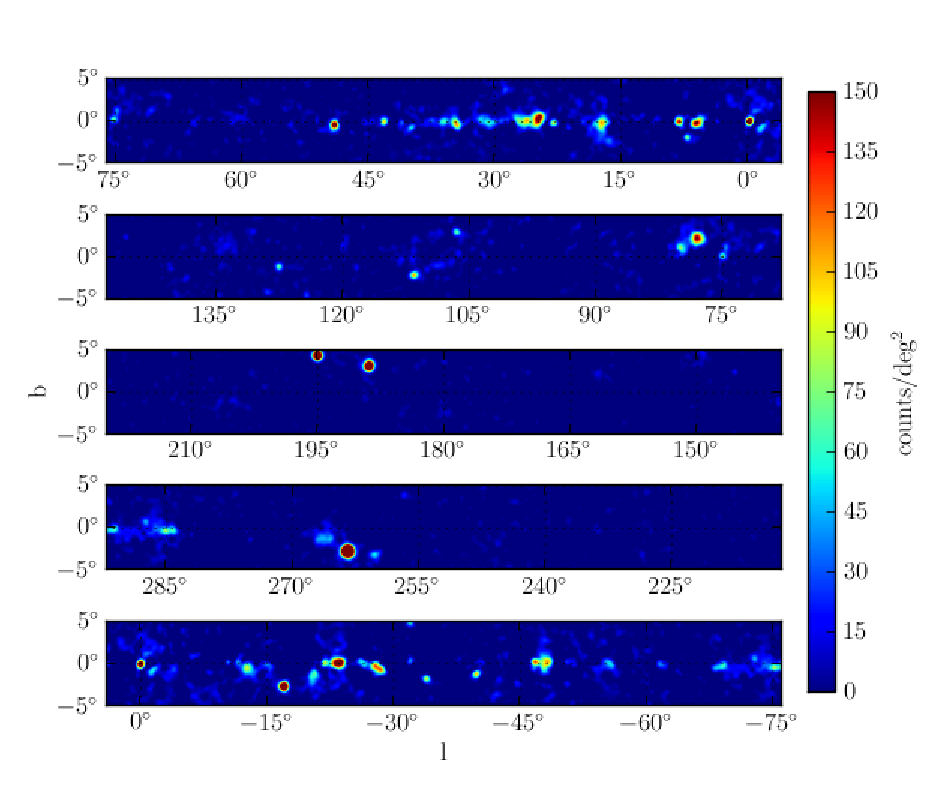
\includegraphics[width=\textwidth]{figures/Plan_gal.eps}
\caption{Residual counts map of the Galactic Plane above 10 GeV. The Galactic and isotropic diffuse emission are subtracted using the files described in section 4.2 with a normalization of 1. All sources associated to Blazars are subtracted using the spectral parameters listed in the hard source list \citep{1FHL}. Excesses visible in this map are due either to Galactic sources or to Blazars not yet associated, emitting above 10 GeV observed by the LAT. The counts map is smoothed with a Gaussian of 0.27$\degr$.
\label{fig:PlanGal}}
\end{figure}

\begin{figure}[h!]
\centering
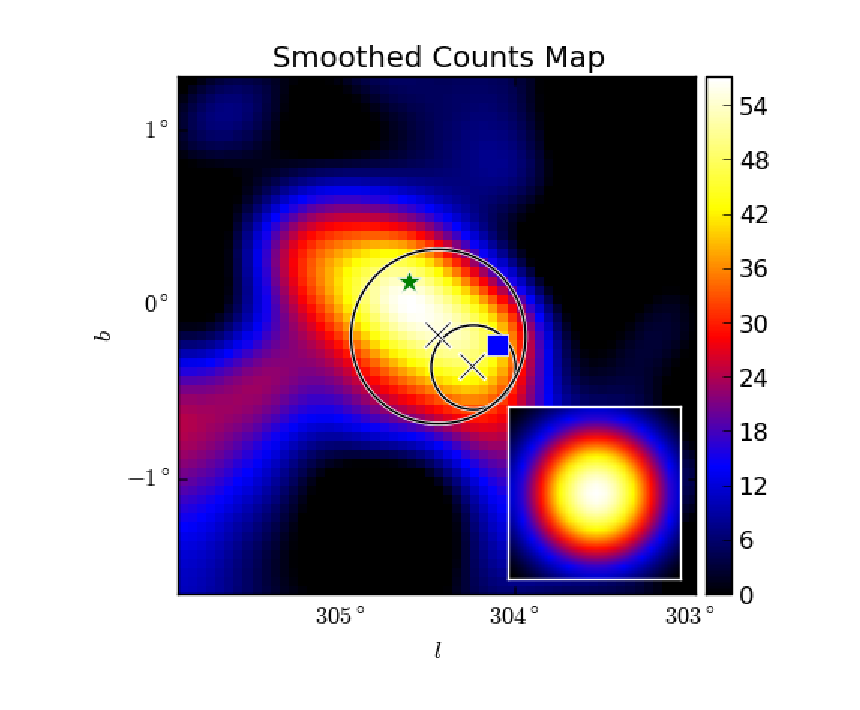
\includegraphics[]{figures/HESSJ1303m631.eps}
\caption{Counts map of the region of HESS~J1303--631. We subtracted the Galactic and isotropic diffuse emission. The counts map is smoothed by a Gaussian of 0.27$\degr$ corresponding to the PSF above 10 GeV. The green star indicates the position of the SNR Kes 17, the blue square represents the position of PSR~J1301--6305. The small and big circles respectively show the extension of the TeV Gaussian proposed by \cite{2005AA...439.1013A} and the extension of the disk derived in this work.
\label{1303}}
\end{figure}

\begin{figure}[h!]
\centering
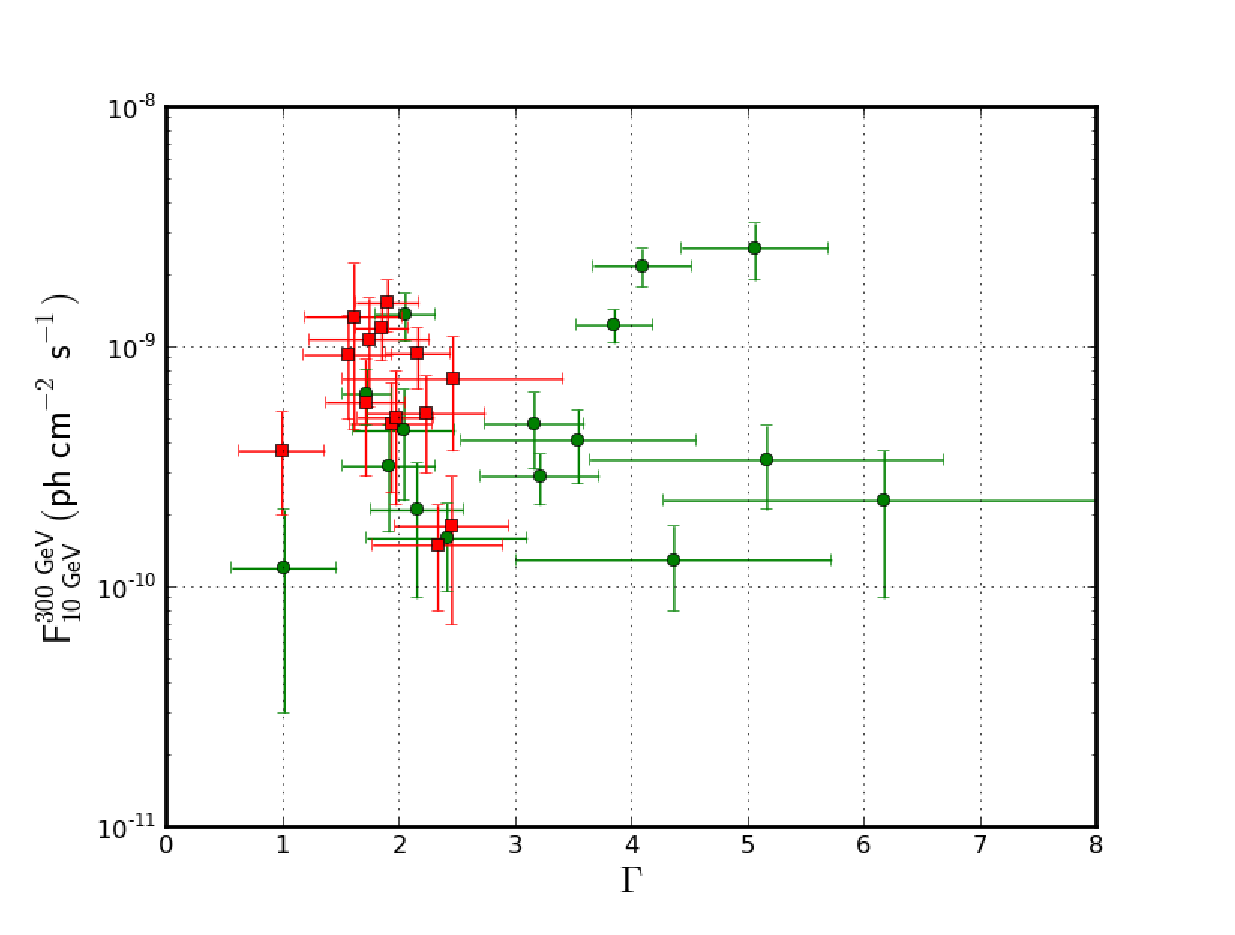
\includegraphics[width=\textwidth]{figures/out_errorbar_best_fit.eps}
\caption{Integrated flux of the detected sources as a function of the power-law index between 10 and 316 GeV (see Table \ref{tab:det_sources}). The green circles show the sources within 0.5$\degr$ of a pulsar detected by the LAT while the red squares represent the sources with no pulsar detected in the GeV energy range within 0.5$\degr$. The error bars show the statistical and systematic uncertainties added in quadrature.  
\label{fig:fluxvssize}}
\end{figure}

\begin{figure}[h!]
\centering
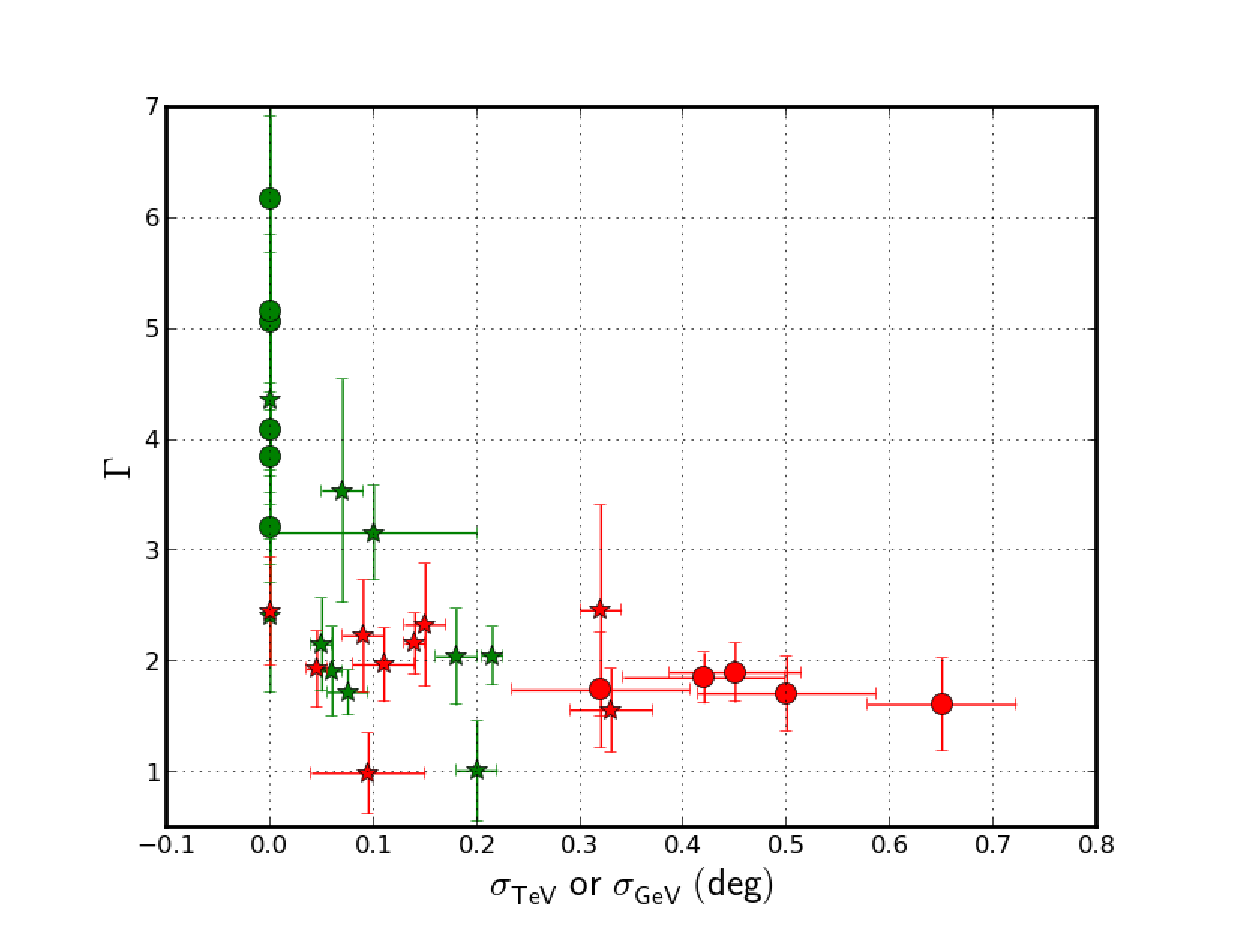
\includegraphics[width=\textwidth]{figures/index_vs_size.eps}
\caption{Spectral index as a function of the GeV or TeV extension for each detected source. The GeV morphology is obtained by fitting the position and extension of the sources as explained in Section \ref{spatanalysis} \& \ref{signi}. The green markers show the sources within 0.5$\degr$ of a pulsar detected by the LAT while the red markers represent the sources with no pulsar detected in the GeV energy range within 0.5$\degr$. The error bars show the statistical and systematic uncertainties added in quadrature. The 11 circles represent the sources for which the GeV morphology significantly improved the fit compared to the TeV morphology (Table \ref{tab:GeVmorph}), while the stars represent the sources modeled assuming their TeV morphology. For sources modelled assuming their TeV morphology, we reported the uncertainties found in the associated reference in Table \ref{tab:TeV_sources}. For asymmetric sources we represented the mean extension with an error bar corresponding to the maximum uncertainty.
\label{fig:indexvssize}}
\end{figure}

%\begin{figure}[h!]
%\centering
%\includegraphics[width=0.5\textwidth]{figures/0FGLJ1958.12848.eps}
%\caption{SED of MGRO J1958$+$2848. The red and blue points show respectively the \emph{Fermi}-LAT and ... points. The black error bars show the statistical and   systematic uncertainties added in quadrature. The black line corresponds to the best fit obtained using the LAT data. The dashed line correspond to the model of PSR J... taken from \cite{2012ApJS..199...31N}.
%\label{fig:1}}
%\end{figure}


\begin{figure}[h!]
\centering
\subfigure{
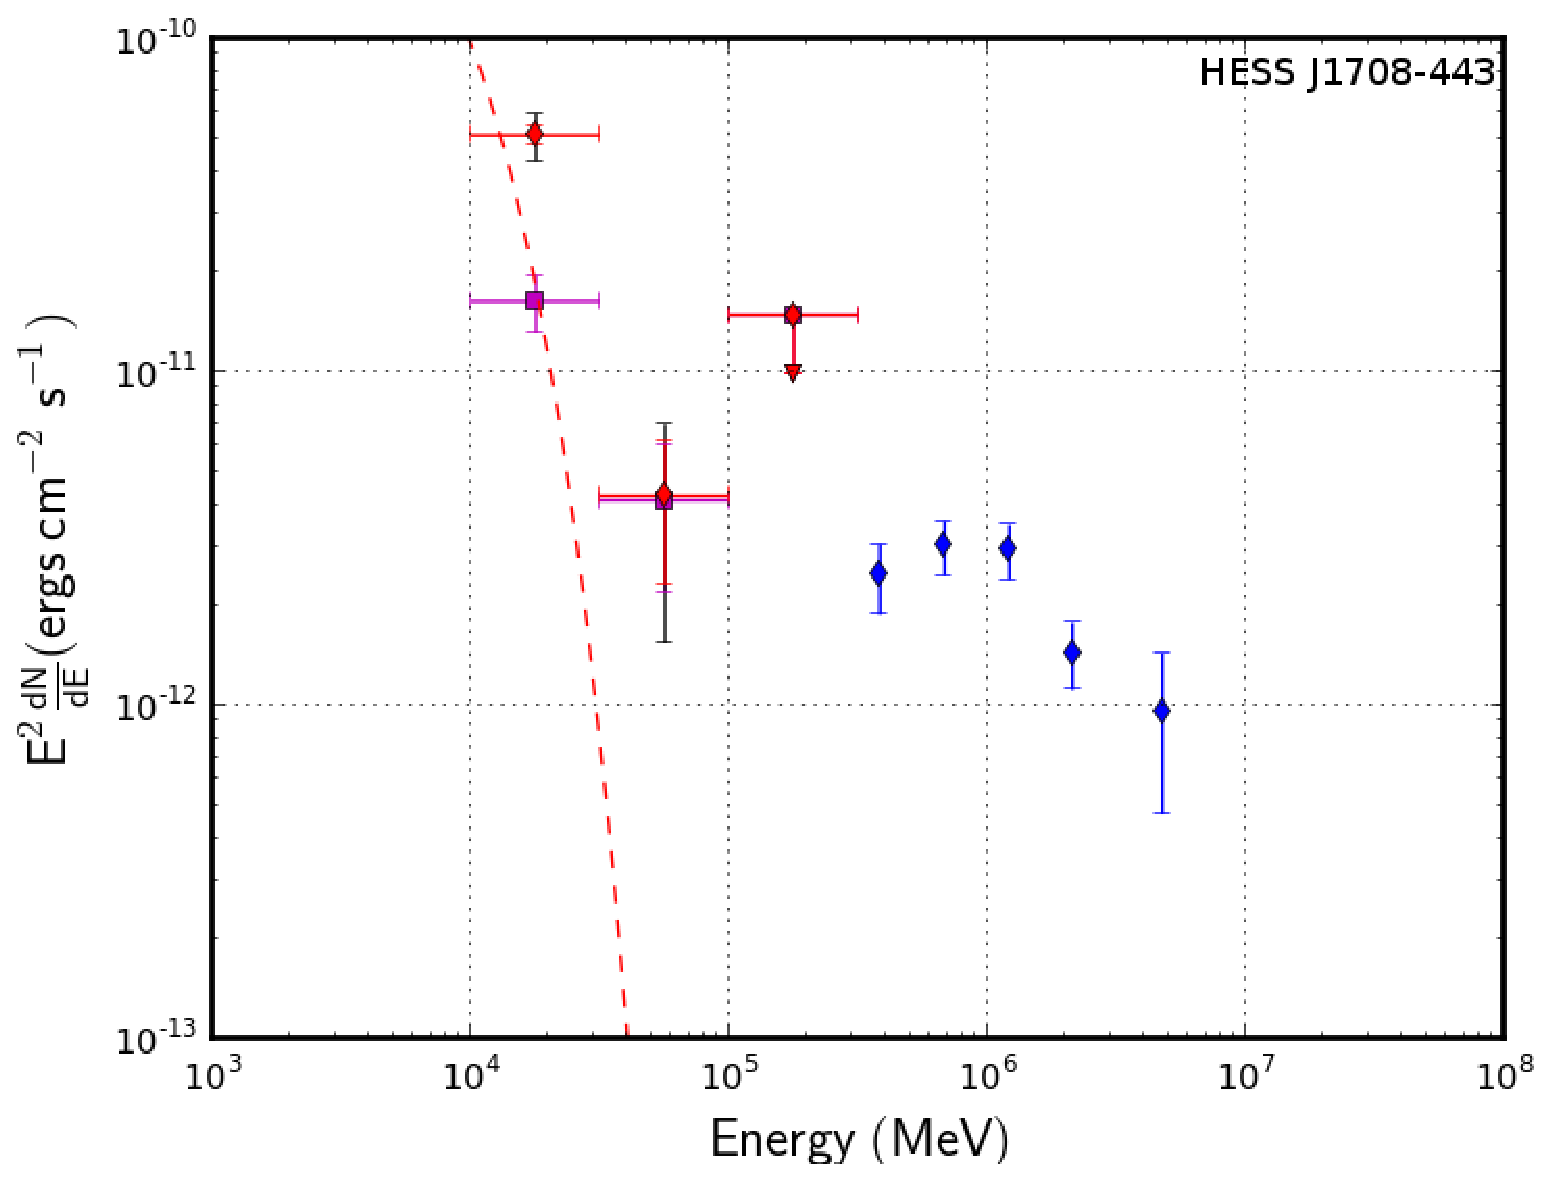
\includegraphics[width=0.45\textwidth]{figures/HESSJ1708.eps}
\label{fig:hess1708}
}
\subfigure{
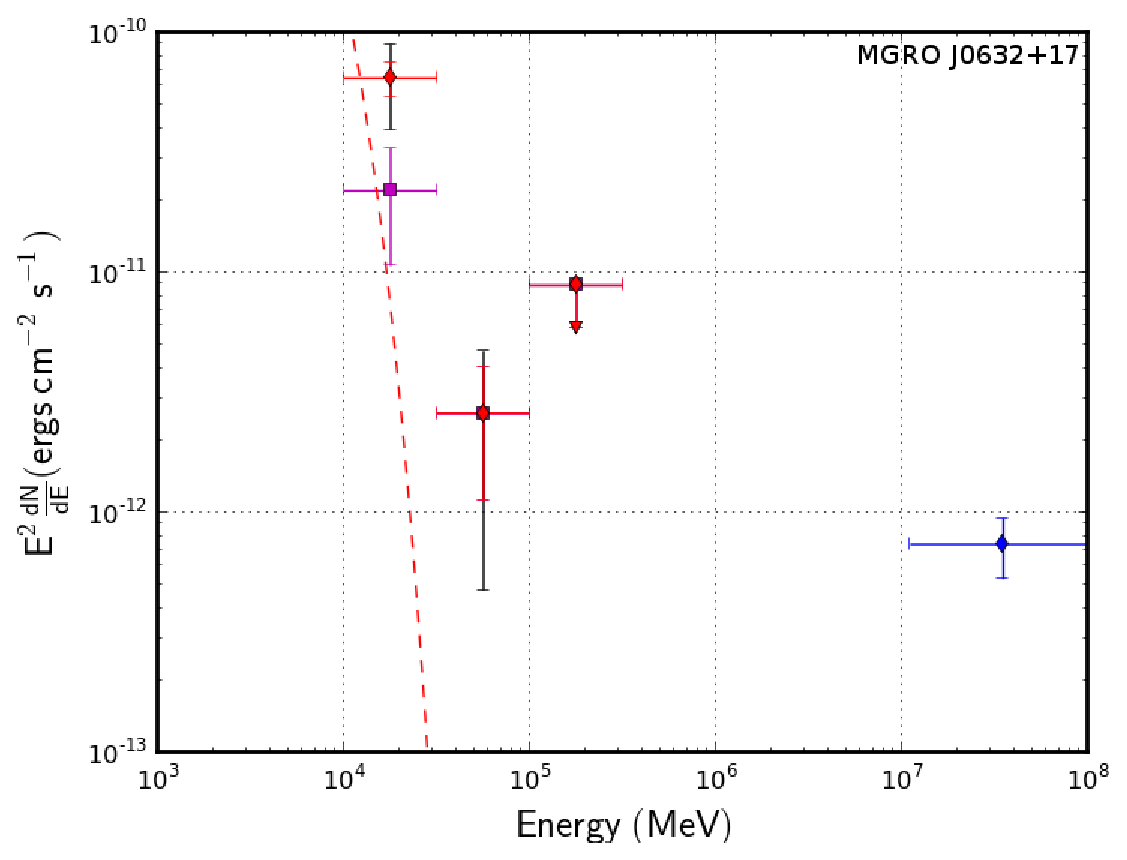
\includegraphics[width=0.45\textwidth]{figures/MGROJ0632.eps}
\label{fig:mgroj0632}
}
\subfigure{
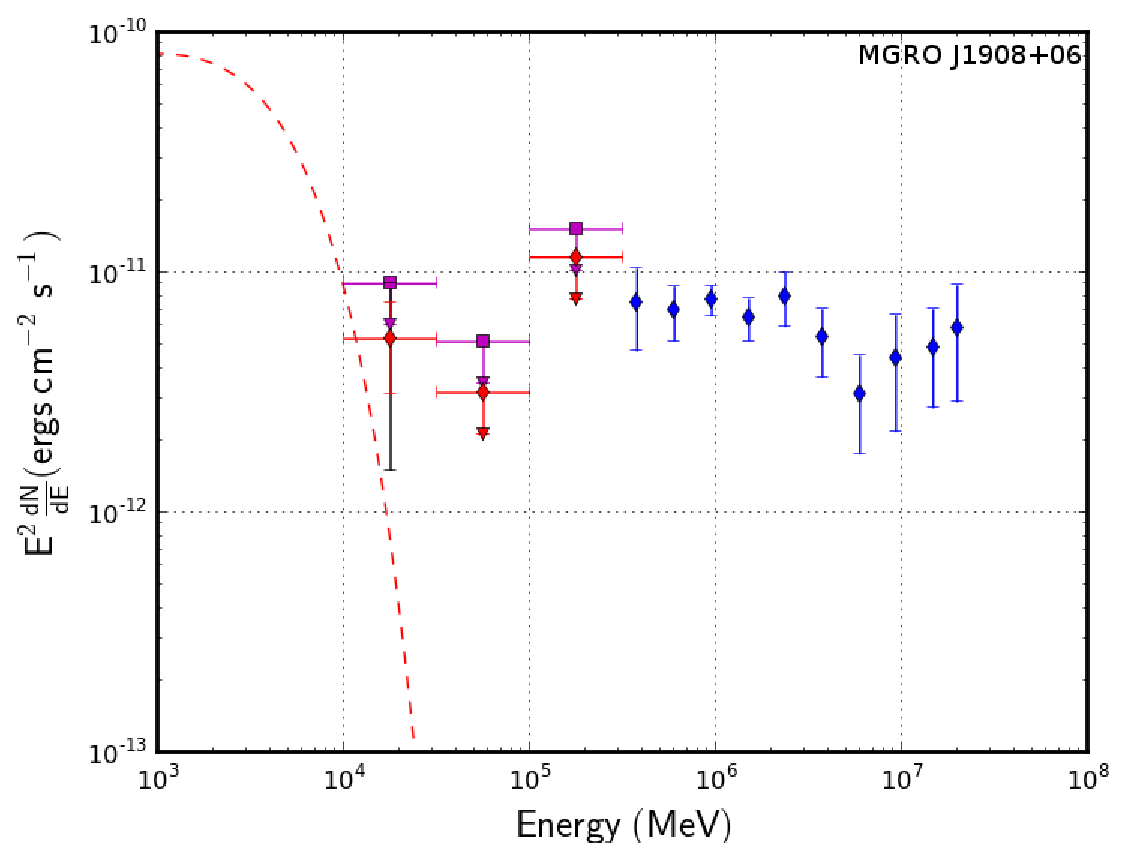
\includegraphics[width=0.45\textwidth]{figures/MGROJ1908.eps}
\label{fig:mgro1908}
}
\subfigure{
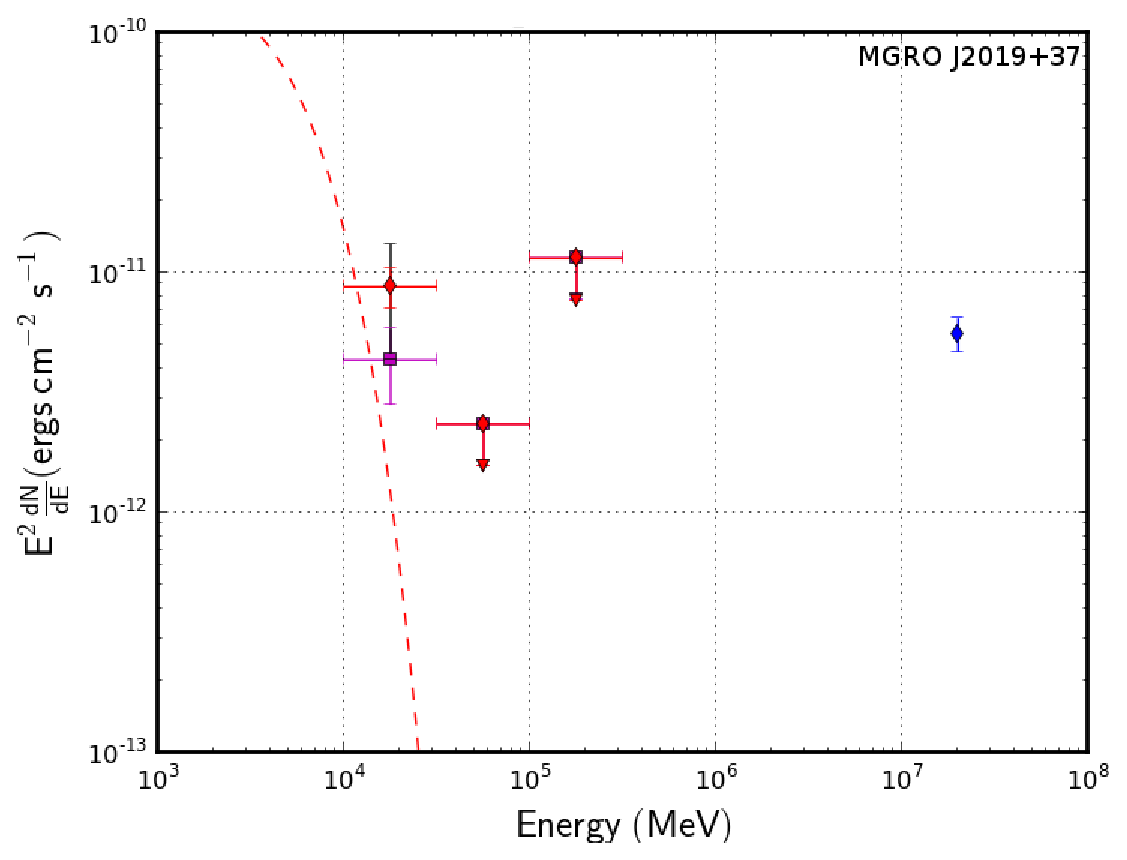
\includegraphics[width=0.45\textwidth]{figures/MGROJ201937.eps}
\label{fig:mgro2019}
}
\subfigure{
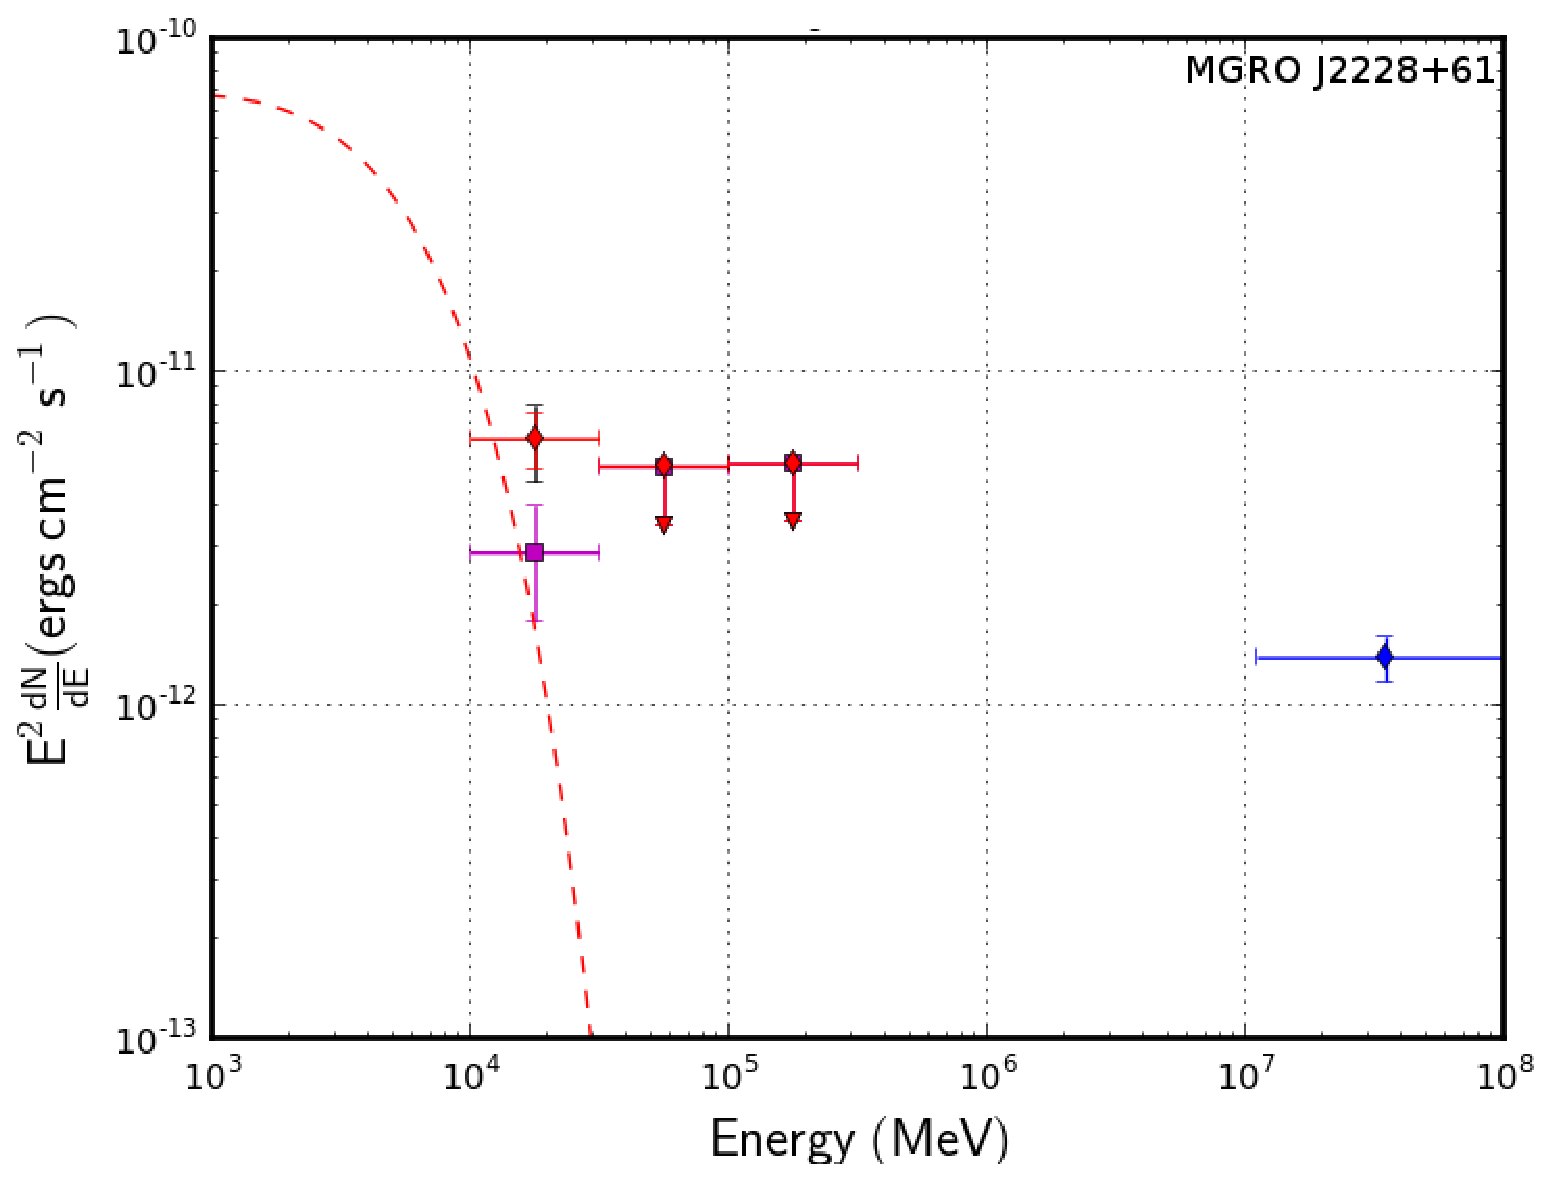
\includegraphics[width=0.45\textwidth]{figures/MGROJ2228.eps}
\label{fig:mgroj2228}
}
\subfigure{
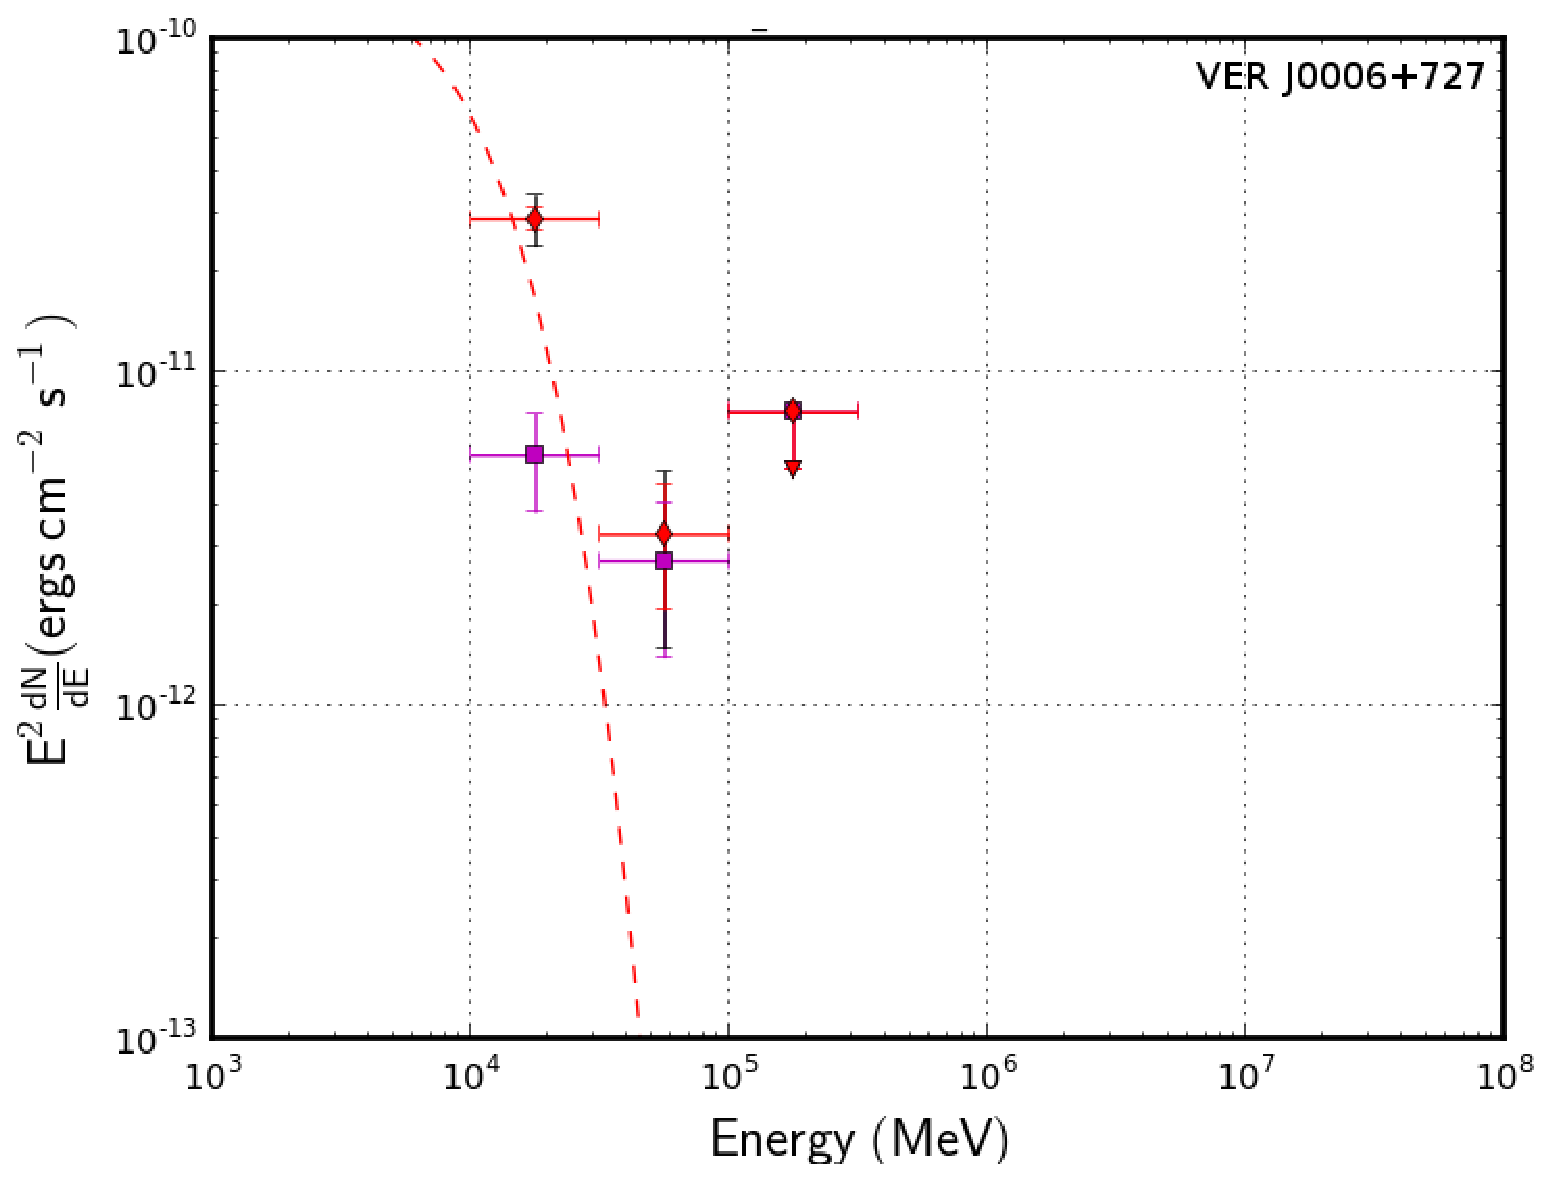
\includegraphics[width=0.45\textwidth]{figures/VERJ0006.eps}
\label{fig:verj0006}
}
\caption{\label{fig:sedsourcespuls}SED of sources better described by a point-like source and with a pulsar within 0.5$\degr$. The blue points show the TeV points taken from \cite{2011AA...528A.143H, 2009ApJ...700L.127A, 2009AA...499..723A, 2007ApJ...664L..91A, 2009ApJ...700L.127A, 2011arXiv1111.2591M}. The red circles and the magenta squares show respectively the SED without the pulsar included in the model and with the pulsar included in the model. The black error bars show the statistical and   systematic uncertainties added in quadrature. The dashed line corresponds to the model of the associated pulsars sumarized in Table \ref{tab:pulsarfit}. In the case of MGRO J1908+06, the red SED was derived assuming a point-like source as determined in Table \ref{tab:GeVmorph} while the magenta SED was derived assuming the TeV shape since it is not significant anymore when the pulsar is included in the model.}
\end{figure}

\begin{figure}[h!]
\centering
\subfigure{
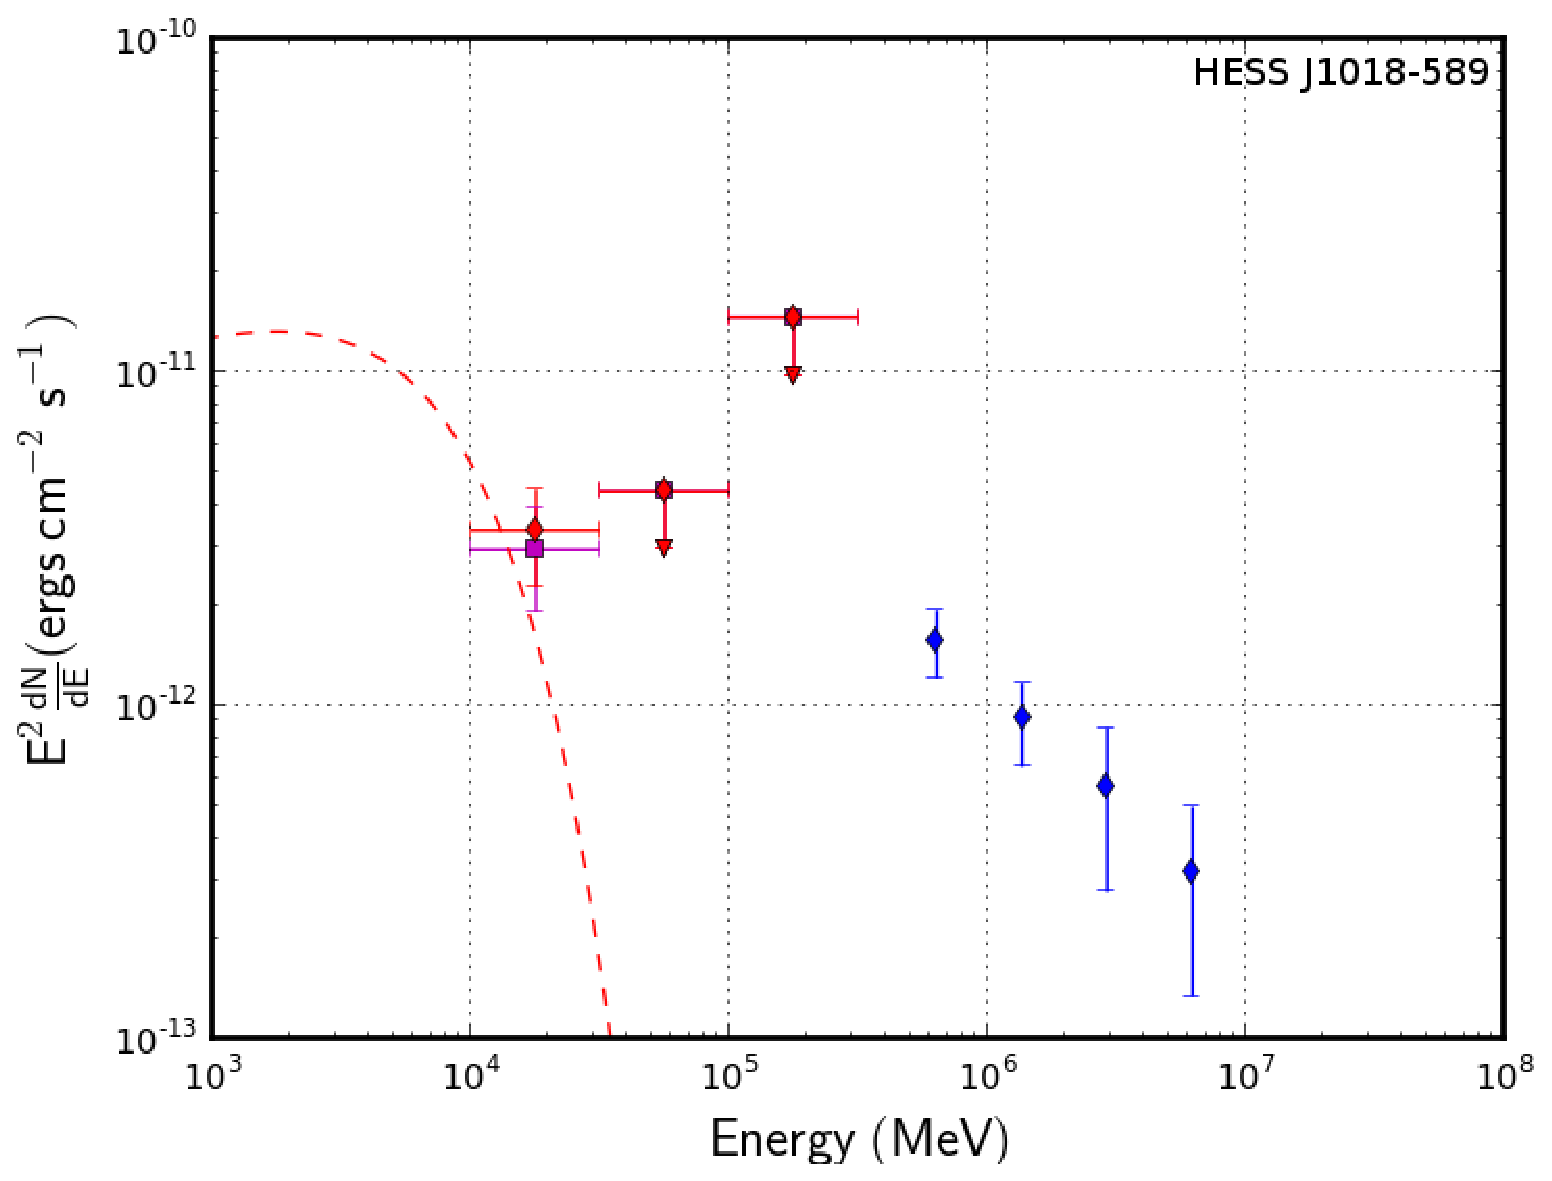
\includegraphics[width=0.45\textwidth]{figures/HESSJ1018.eps}
\label{fig:hessj1018}
}
\subfigure{
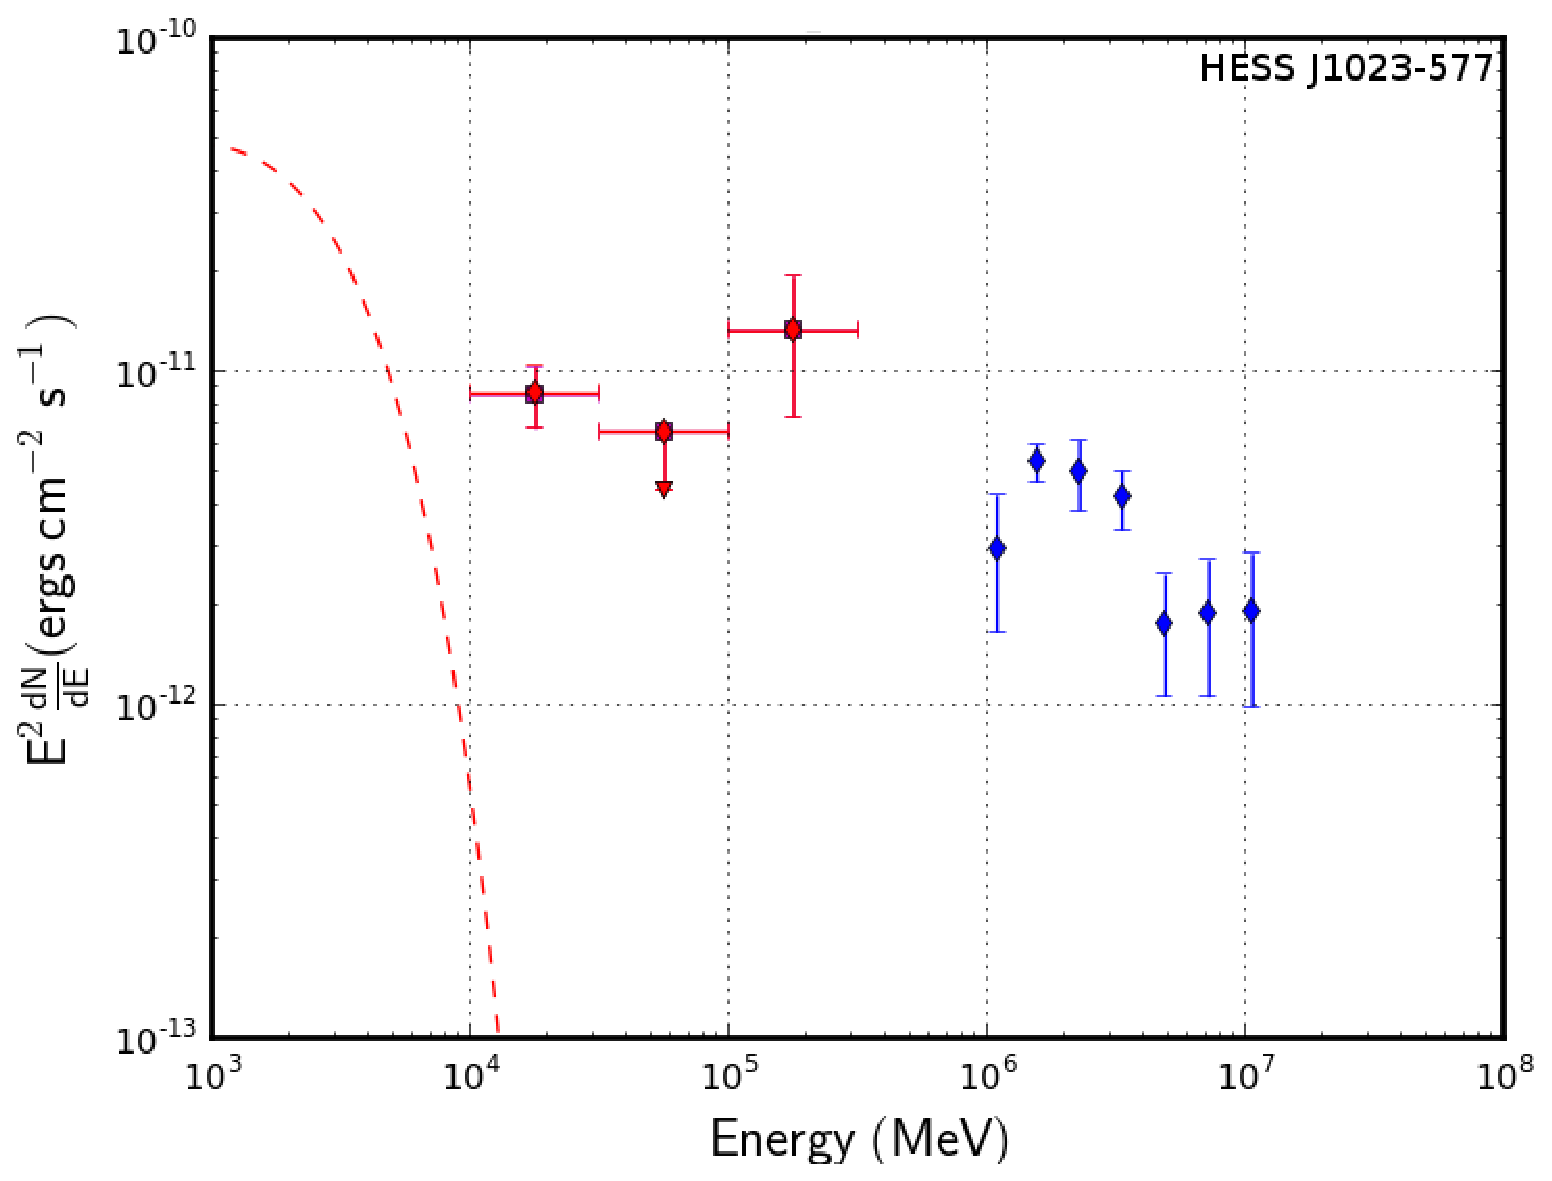
\includegraphics[width=0.45\textwidth]{figures/HESSJ1023.eps}
\label{fig:hessj1023}
}
\subfigure{
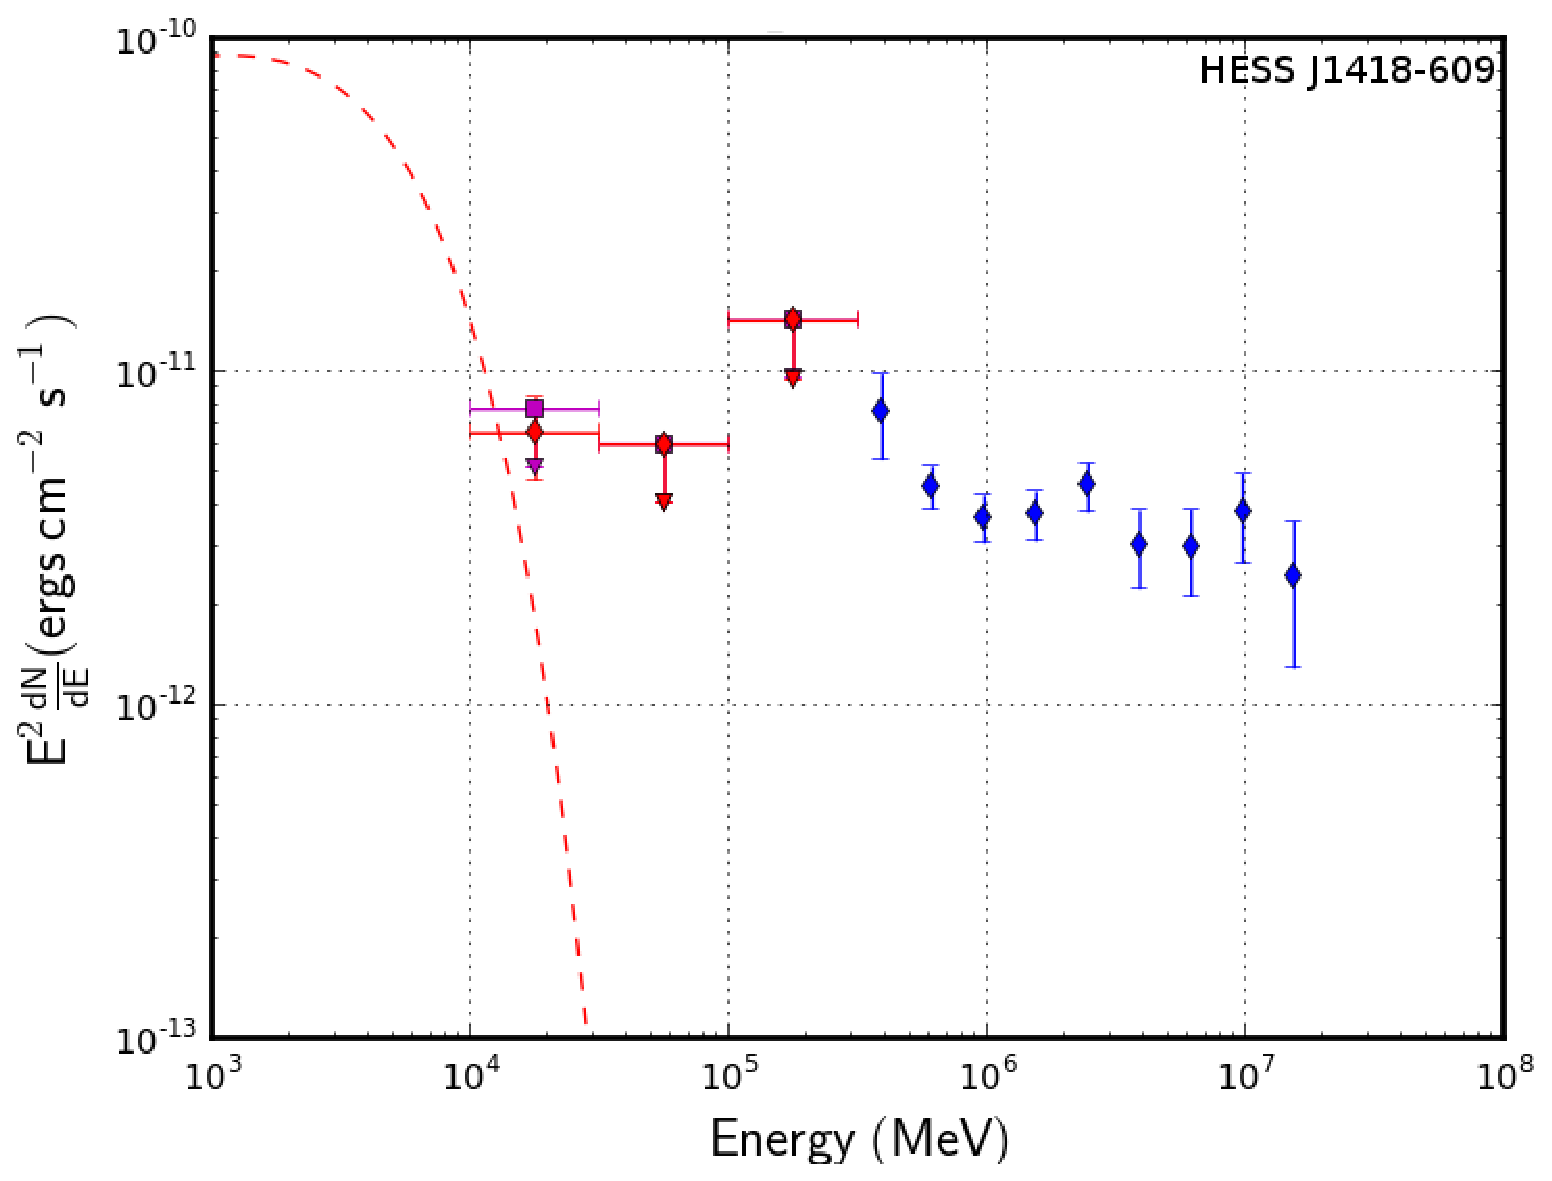
\includegraphics[width=0.45\textwidth]{figures/HESSJ1418.eps}
\label{fig:hessj1418}
}
\subfigure{
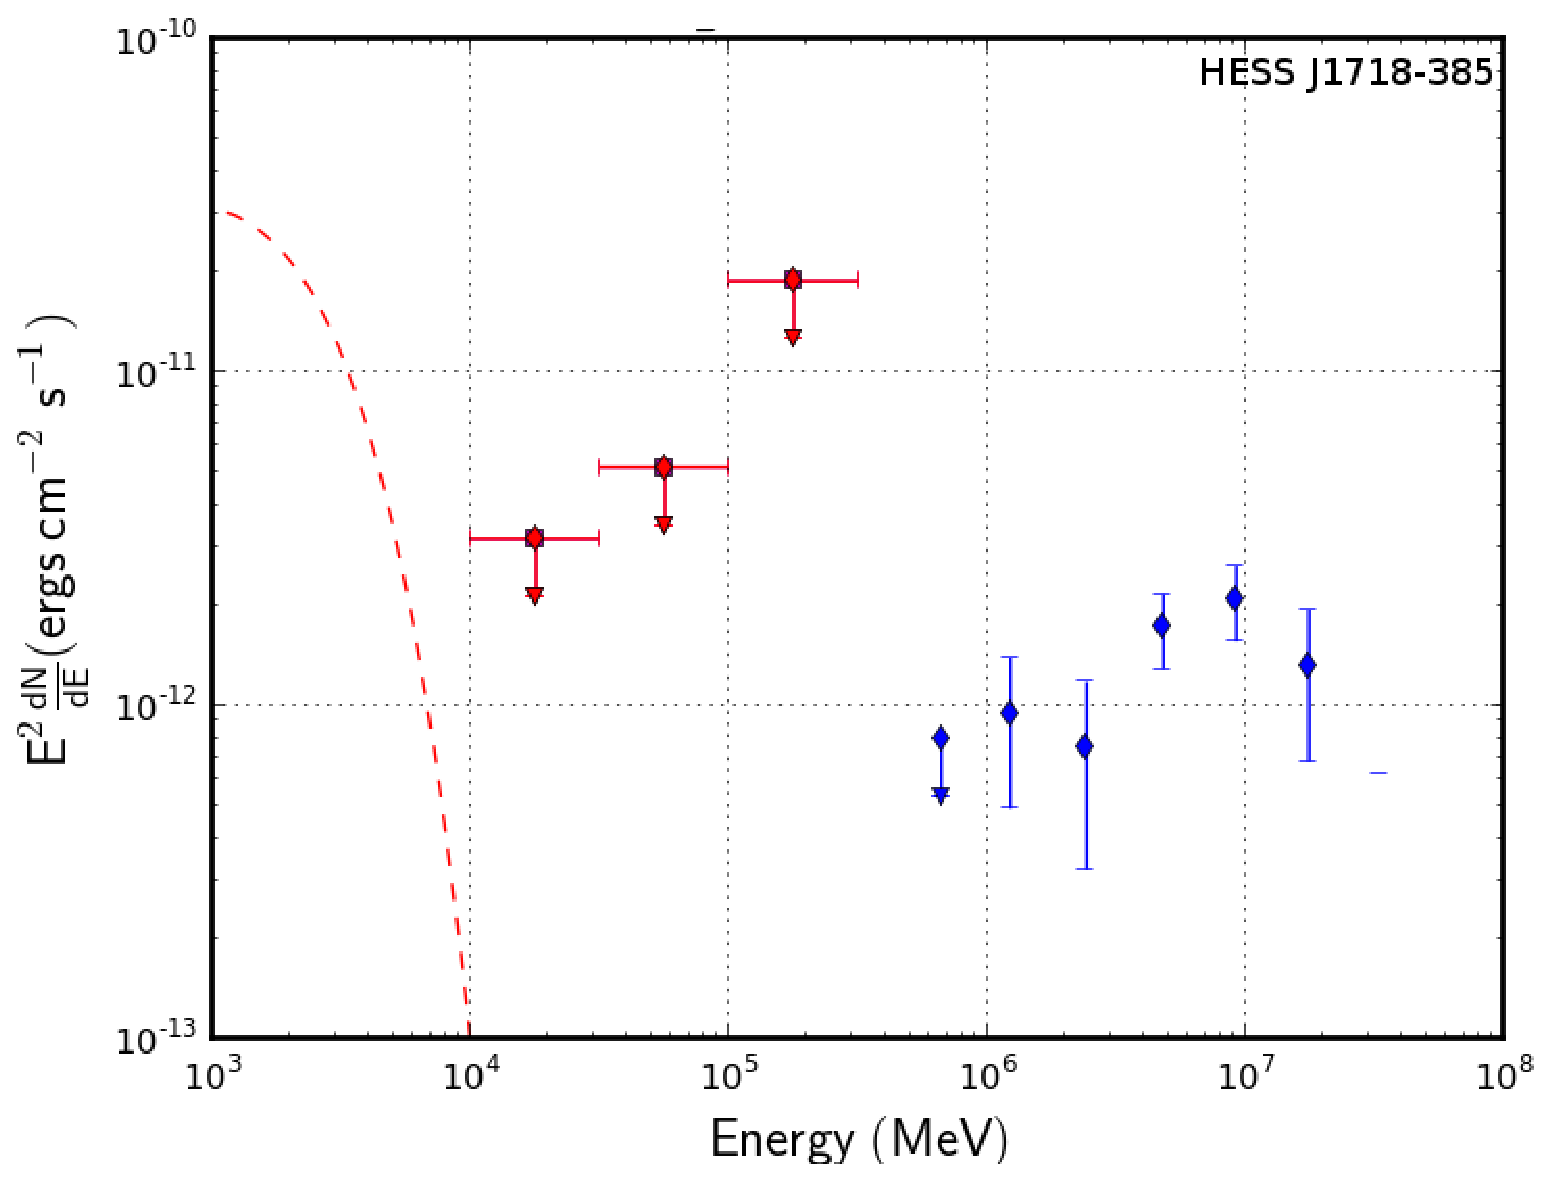
\includegraphics[width=0.45\textwidth]{figures/HESSJ1718.eps}
\label{fig:hessj1718}
}
\caption{\label{fig:sedsourcespuls2}SED of sources better described by the TeV shape and with a pulsar within 0.5$\degr$. The blue points show the TeV points taken from the associated paper in Table \ref{tab:TeV_sources}. The red circles and the magenta squares show respectively the SED without the pulsar included in the model and with the pulsar included in the model. The black error bars show the statistical and   systematic uncertainties added in quadrature. The dashed line corresponds to the model of the associated pulsars sumarized in Table \ref{tab:pulsarfit}.}
\end{figure}

\begin{figure}[h!]
\centering

\subfigure{
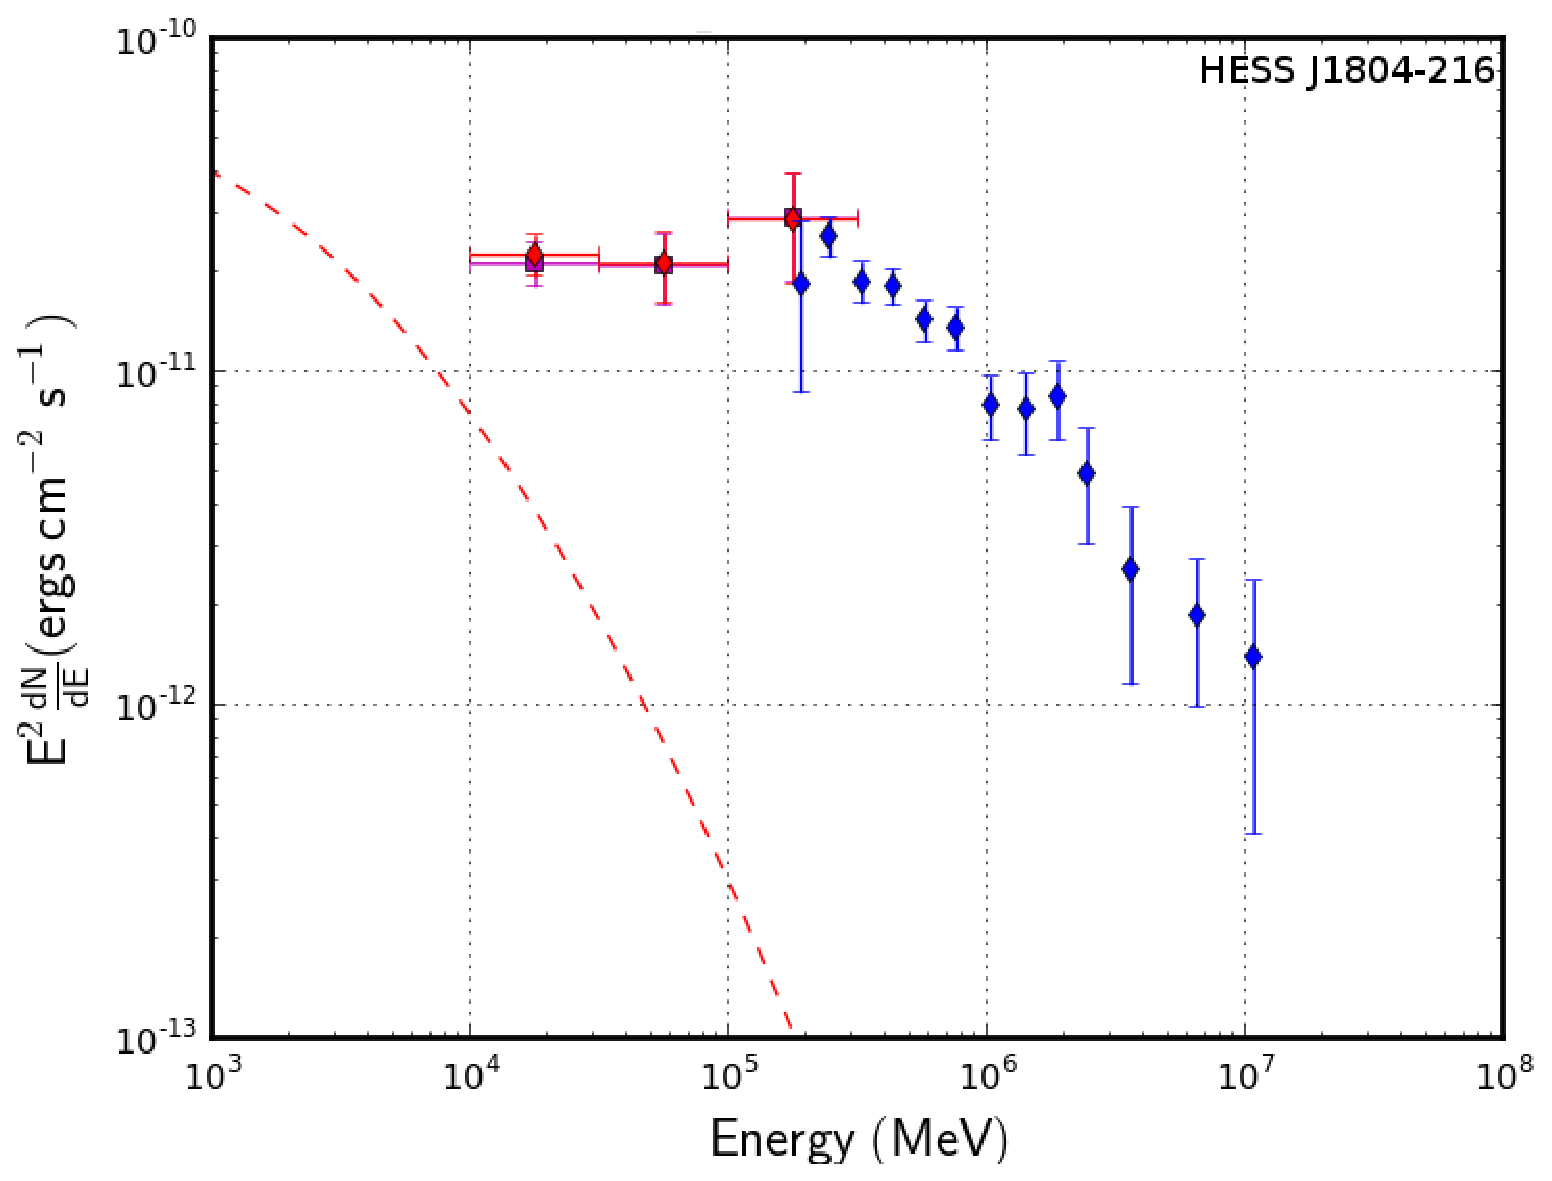
\includegraphics[width=0.45\textwidth]{figures/HESSJ1804.eps}
\label{fig:hessj1804}
}
\subfigure{
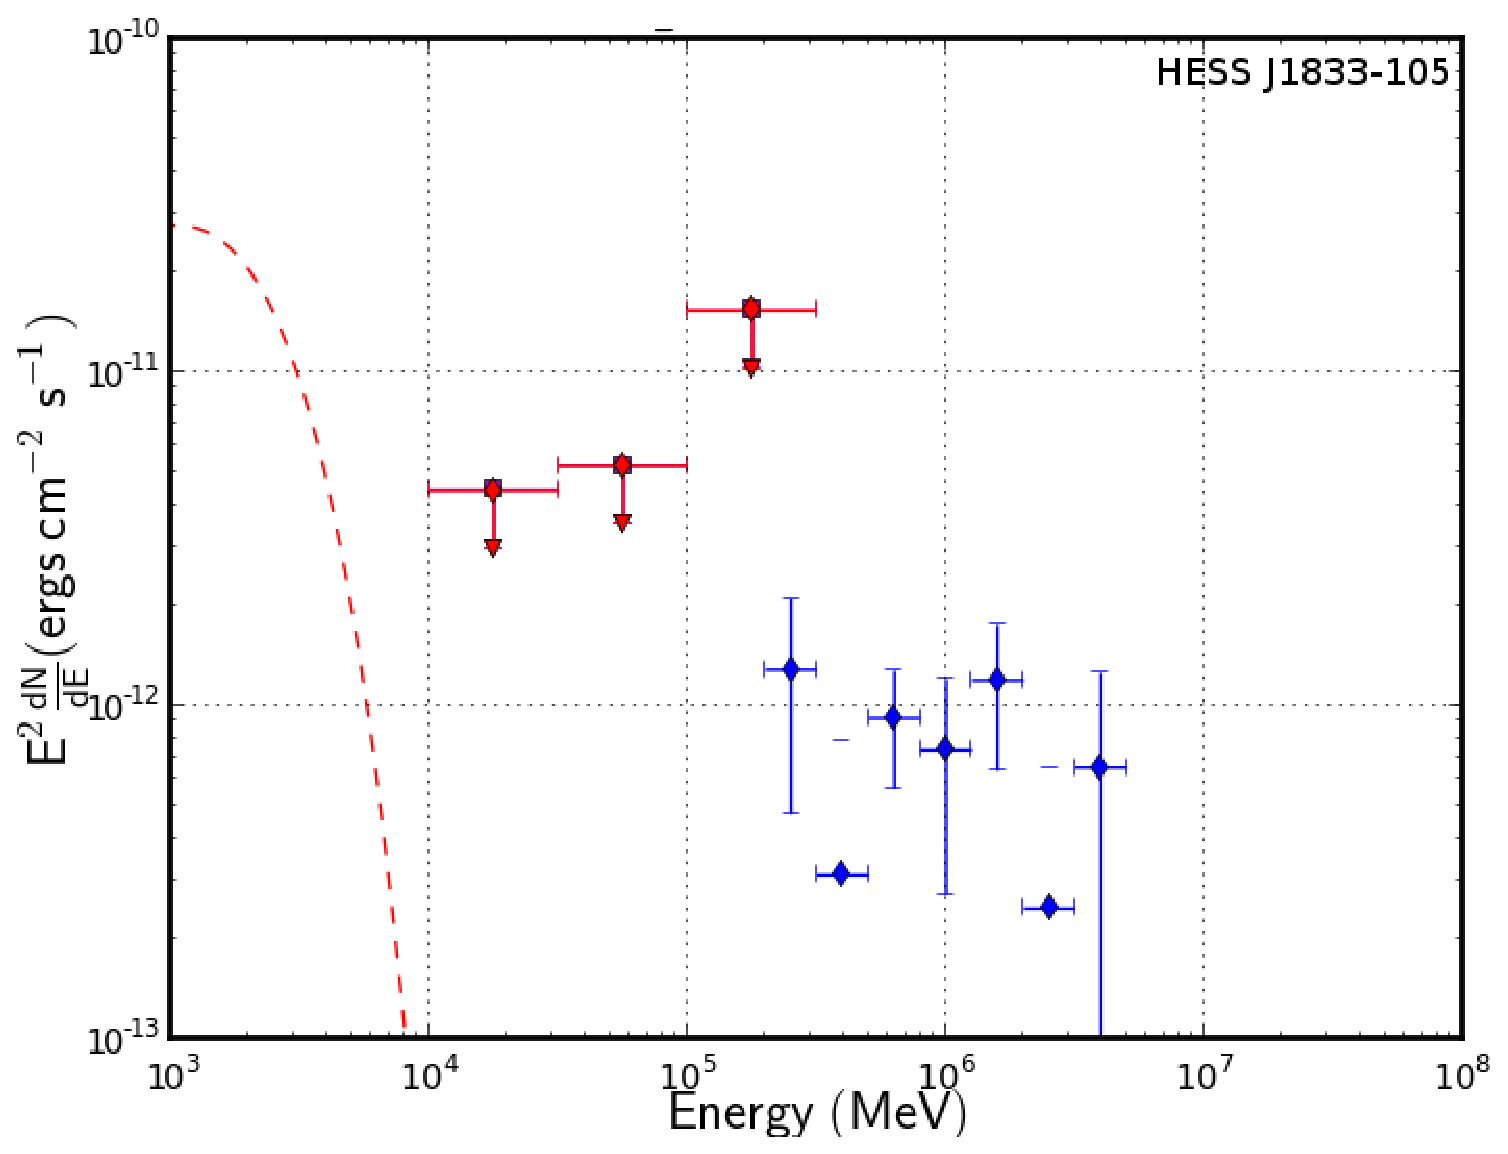
\includegraphics[width=0.45\textwidth]{figures/HESSJ1833.eps}
\label{fig:hess1833}
}
\subfigure{
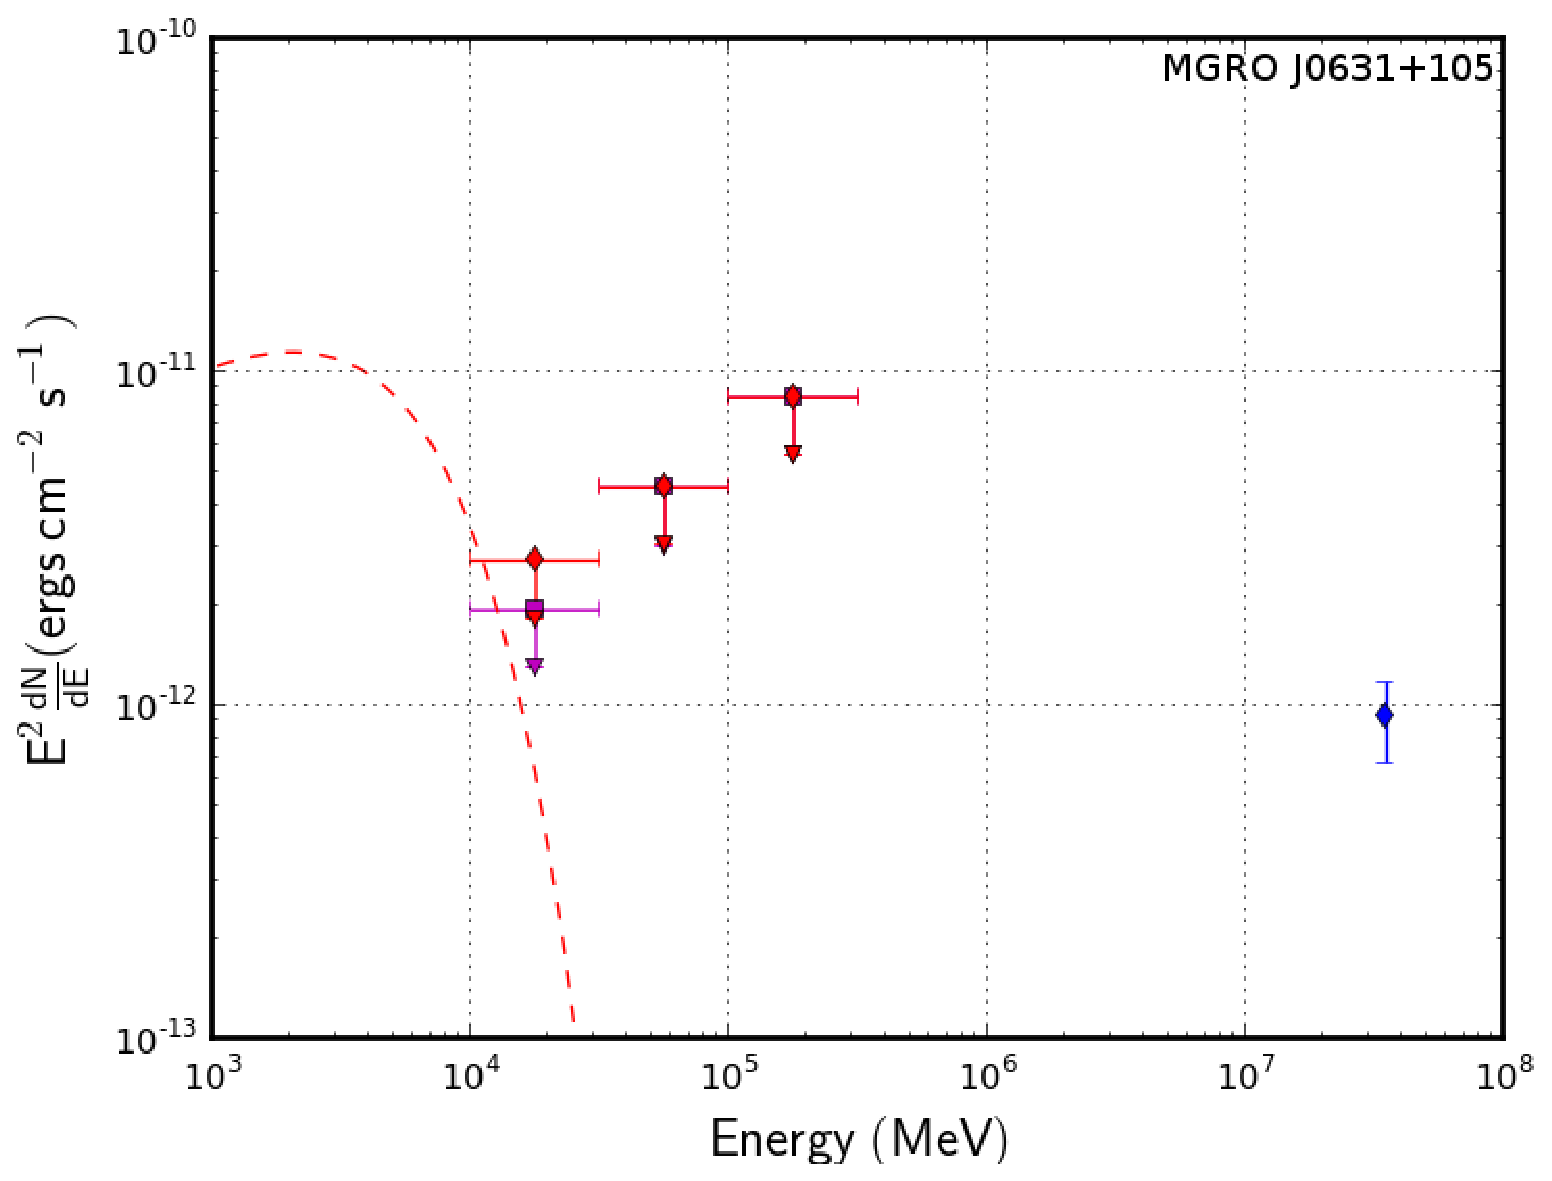
\includegraphics[width=0.45\textwidth]{figures/MGROJ0631.eps}
\label{fig:mgroj0631}
}
\subfigure{
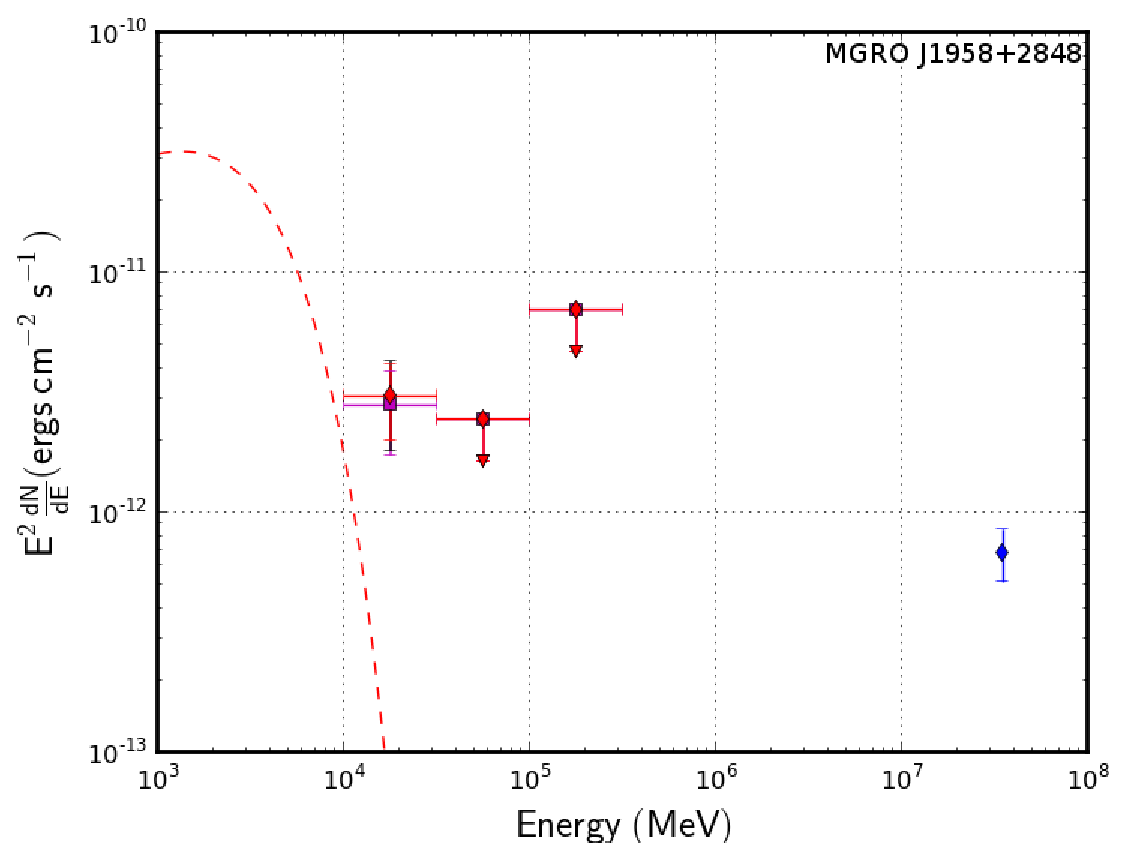
\includegraphics[width=0.45\textwidth]{figures/MGROJ1958.eps}
\label{fig:mgroj1958}
}

\caption{\label{fig:sedsourcespuls3}SED of sources better described by the TeV shape and with a pulsar within 0.5$\degr$. The blue points show the TeV points taken from the associated paper in Table \ref{tab:TeV_sources}. The red circles and the magenta squares show respectively the SED without the pulsar included in the model and with the pulsar included in the model. The black error bars show the statistical and   systematic uncertainties added in quadrature. The dashed line corresponds to the model of the associated pulsars summarized in Table. \ref{tab:pulsarfit}.}
\end{figure}

\clearpage

\begin{figure}[h!]
\centering
\subfigure{
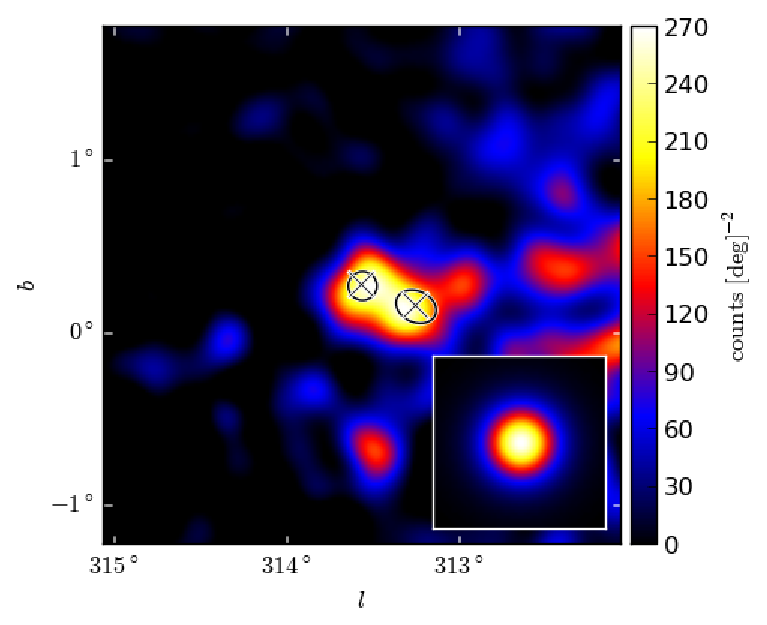
\includegraphics[width=0.60\textwidth]{figures/K310GeV.eps}}
\subfigure{
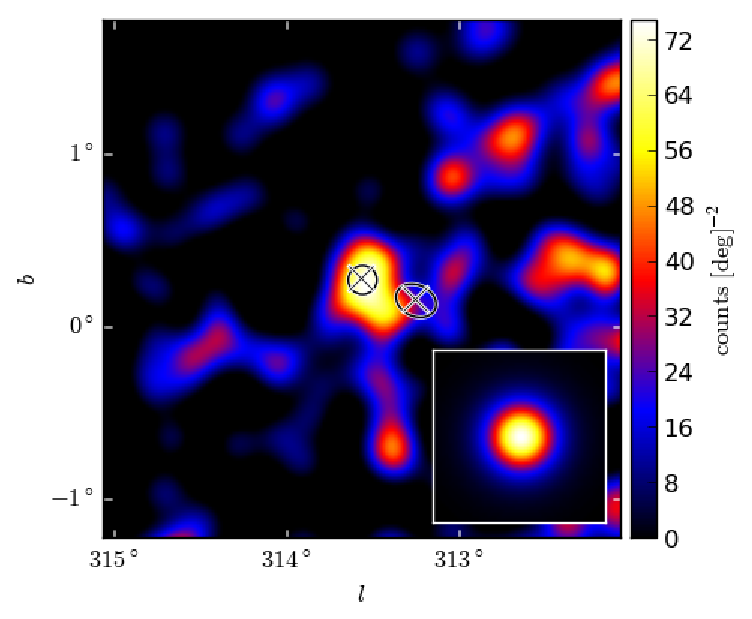
\includegraphics[width=0.60\textwidth]{figures/K330GeV.eps}}
\caption{Smoothed counts map of the region of the Kookaburra complex observed by Fermi above 10 GeV (Top) and
30 GeV (Bottom). The Galactic diffuse emission is subtracted. The circle and right ellipse show the best fit obtained in TeV respectively for the K3 nebula and the Rabbit nebula.
\label{fig:K3countsmap}}
\end{figure}

\clearpage

\begin{figure}[h!]
\centering
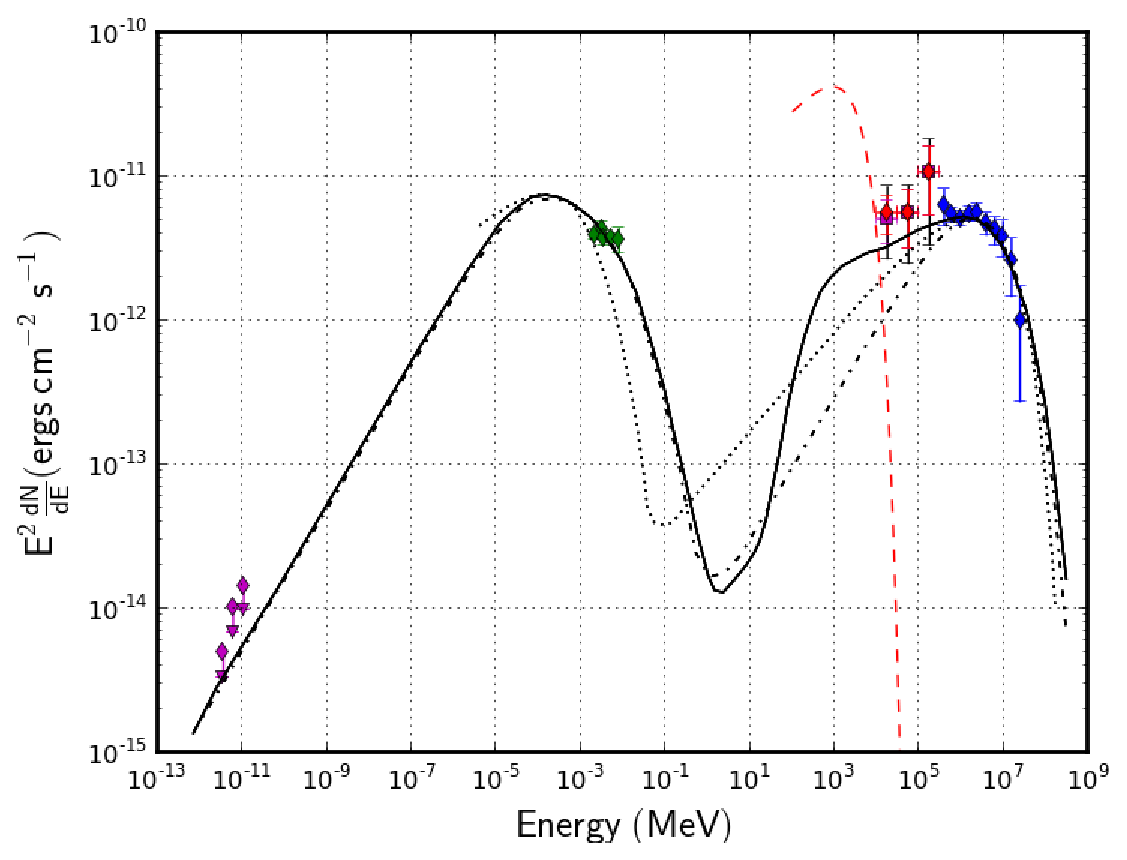
\includegraphics[width=0.60\textwidth]{figures/HESSJ1420.eps}
\caption{SED of HESS J1420-607. The blue, green and magenta points respectively show the spectral points obtained by HESS \citep{2006AA...456..245A}, by Suzaku \citep{2010ApJ...711.1168V} and the upper limits derived in radio. The red points and the magenta squares show the spectral points obtained in this work without and with the pulsar included in the model. In the LAT energy range the black error bars show the statistical and systematic uncertainties added in quadrature. The red dashed line corresponds to the 2FGL spectrum of the PSR J1420-607. The three black lines show the results of SED modeling for the broad extended nebula emission presented in previous works. The solid and dot dashed lines respectively shows to the hadronic plus leptonic and leptonic models proposed by \cite{2010ApJ...711.1168V}. The dotted line corresponds to the leptonic model proposed by \cite{2012ApJ...750..162K} assuming an ambient magnetic field of 3$\mu$G.
\label{fig:hessj1420}}
\end{figure}

\begin{figure}[h!]
\centering
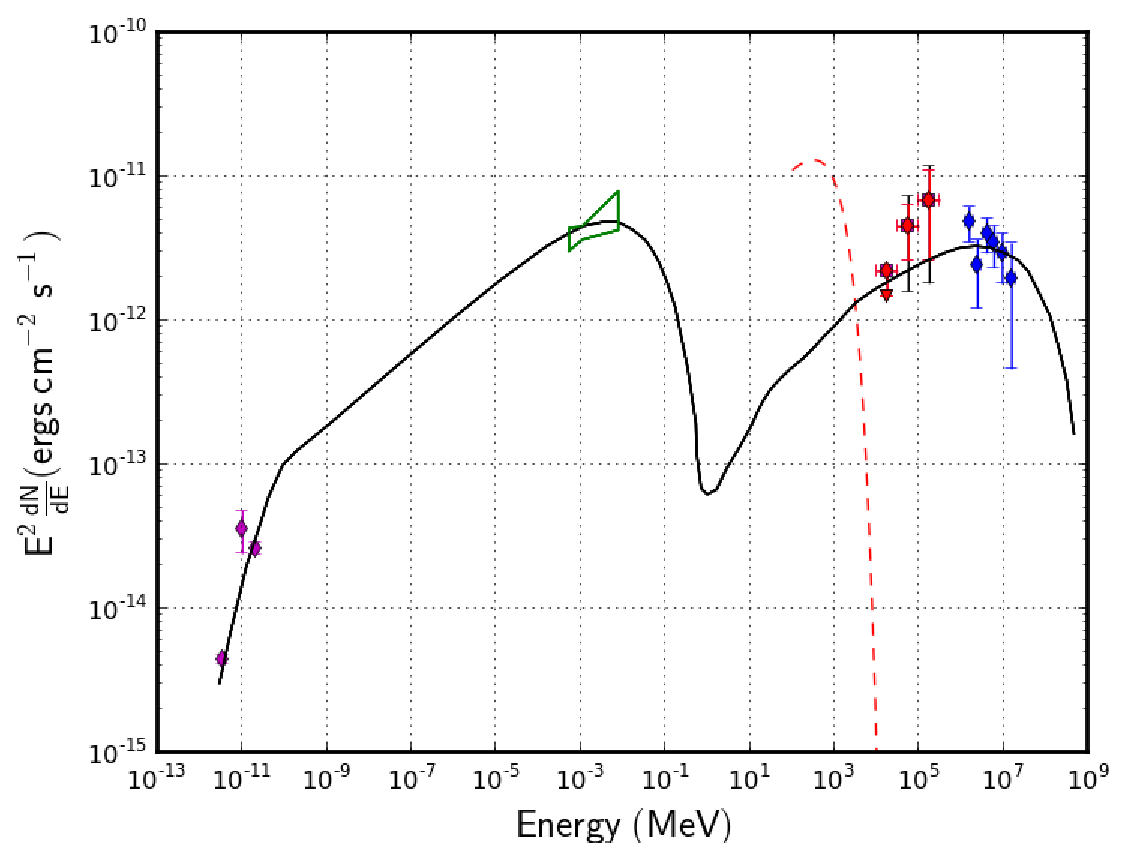
\includegraphics[width=0.60\textwidth]{figures/HESSJ1356.eps}
\caption{SED of HESS J1356-645. The blue, green and magenta points represents the results obtained by HESS \citep{2011AA...533A.103H}, the X-ray data \citep{2011AA...533A.102L} and the radio data \citep{2007MNRAS.382..382M, 1995MNRAS.277...36D, 1993AJ....105.1666G}. The red and magenta points between 10 and 316 GeV show the points obtained in this work without and with PSR J1357-6429 included in the model. In the LAT energy range the red and black error bars respectively show the statistical and systematic uncertainties added in quadrature. The solid line presents the one-zone leptonic model proposed by \cite{2011AA...533A.103H}.
\label{fig:hess1356}}
\end{figure}

\begin{figure}[h!]
\centering
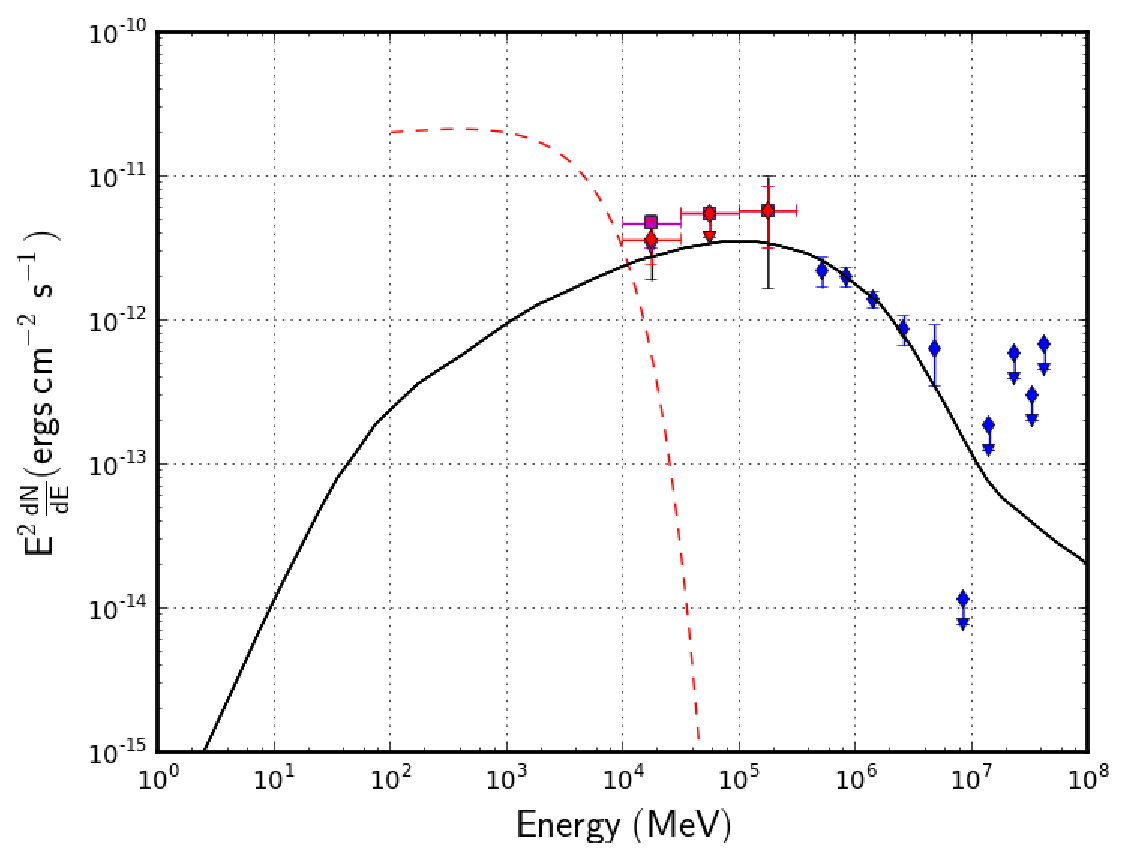
\includegraphics[width=0.60\textwidth]{figures/HESSJ1119.eps}
\caption{SED of HESS J1119$-$614. The blue points represent the HESS data \citep{Mayerdiploma}. The red and magenta points between 10 and 316 GeV show the points obtained in this work without and with PSR J1119$-$6127 included in the model. In the LAT energy range the red and black error bars respectively show the statistical and systematic uncertainties added in quadrature. The solid line shows the model proposed by \cite{Mayerdiploma}. The red dashed line corresponds to the model of PSR~J1119$-$6127 \citep{2012ApJS..199...31N}.
\label{fig:hessj1119}}
\end{figure}



\begin{figure}[h!]
\centering
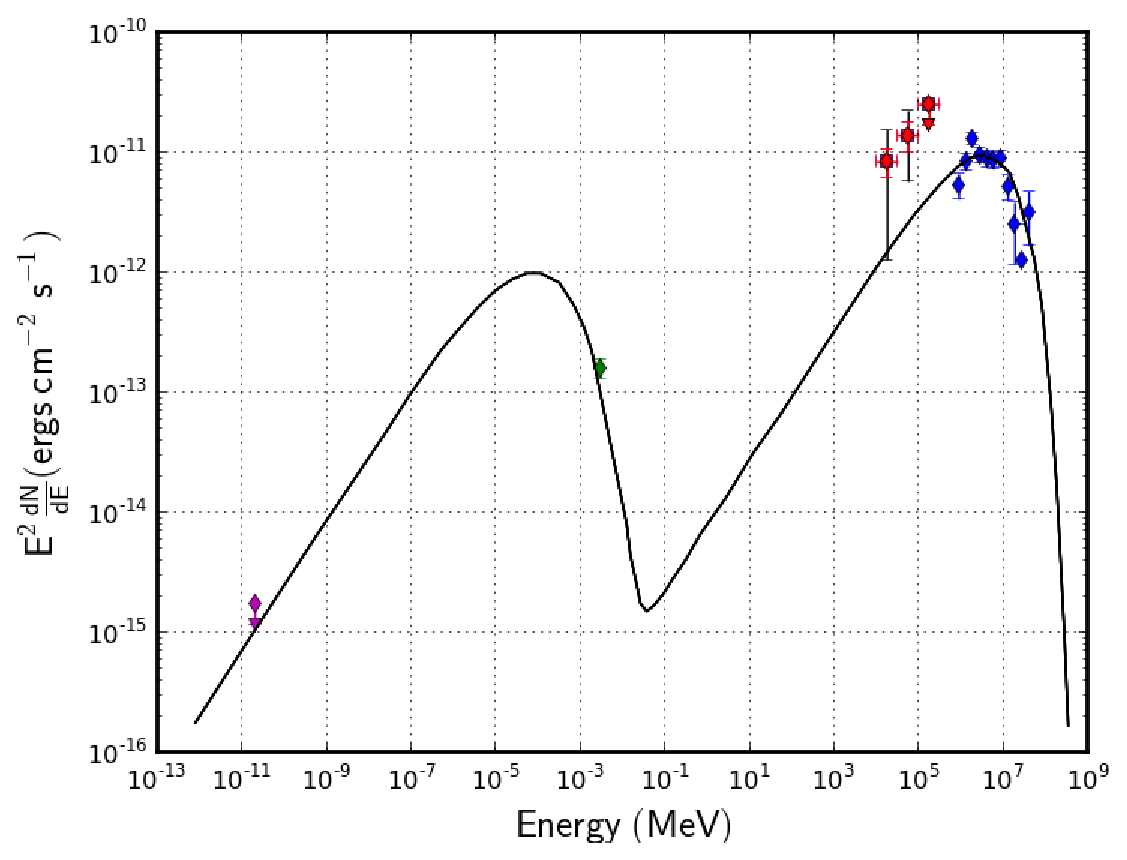
\includegraphics[width=0.60\textwidth]{figures/HESSJ1303631.eps}
\caption{SED of HESS J1303-631. The blue, green and magenta points represents HESS results, the radio data and \emph{Chandra} results \citep{dalton1303}. In the LAT energy range the red and black error bars respectively show the statistical and systematic uncertainties added in quadrature. The solid line shows the leptonic model proposed by \cite{dalton1303}.
\label{fig:hessj1303}}
\end{figure}


\begin{figure}[h!]
\centering
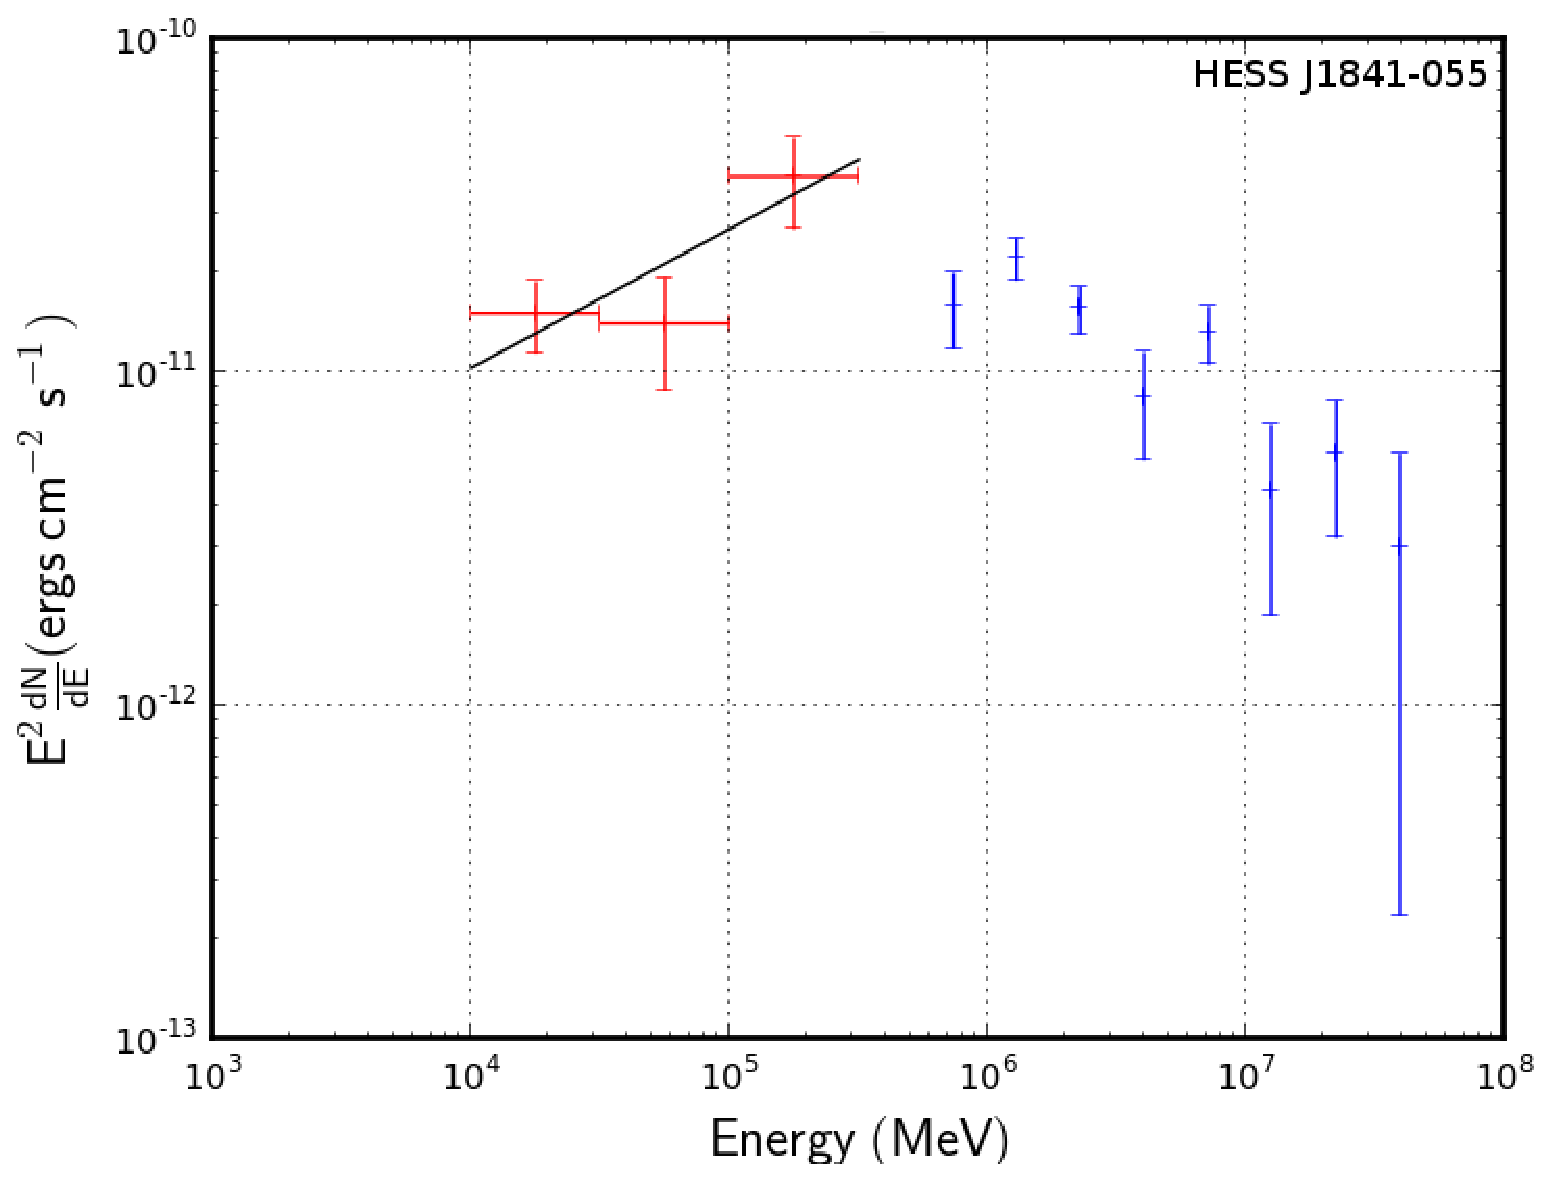
\includegraphics[width=0.60\textwidth]{figures/HESSJ1841055.eps}
\caption{SED of HESS~J1841$-$055. We reported the spectral points obtained using H.E.S.S. data in blues as well as the \emph{Fermi}-LAT spectral points in red. The red and black error bars respectively show the statistical and systematic uncertainties added in quadrature.
\label{fig:1841}}
\end{figure}

\begin{figure}[h!]
\centering
\includegraphics[width=0.60\textwidth]{figures/HESSJ1848018.eps}
\caption{SED of HESS~J1848$-$018. H.E.S.S. pectral points from \cite{chavesthesis} are presented in blue while the radio points corresponding to the W43 central cluster from \cite{2011AA...532A..92L} are indicated in magenta. Red points represent \emph{Fermi}-LAT data. The red and black error bars respectiveley show the statistical uncertainties and statistical plus systematic uncertainties added in quadrature. The red dashed line corresponds to the SED derived in \cite{2011MmSAI..82..739L} using \emph{Fermi}-LAT data and assuming a Gaussian shape of 0.3$\degr$.
\label{fig:1848}}
\end{figure}

\begin{figure}[h!]
\centering
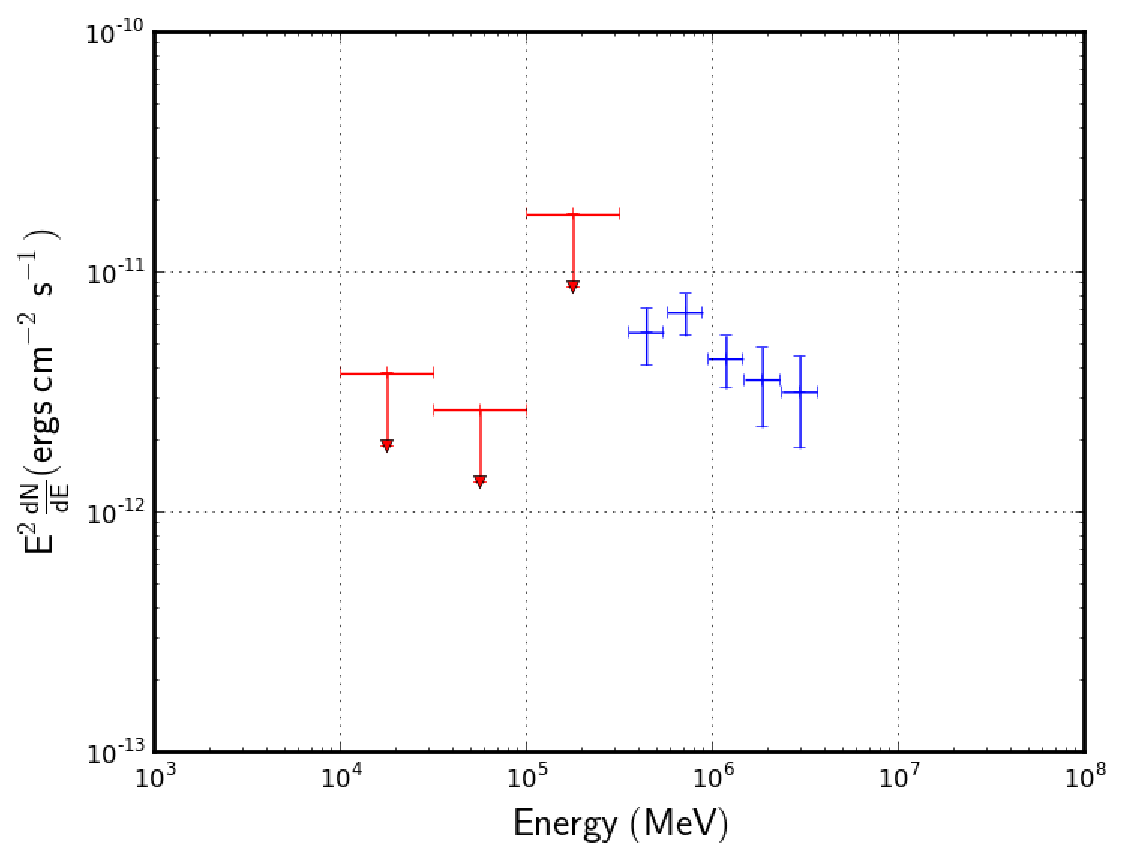
\includegraphics[width=0.60\textwidth]{figures/HESSJ1026.eps}
\caption{SED of HESS~J1026$-$582. H.E.S.S. spectral points are reported in blue while \emph{Fermi}-LAT upper limits are indicated in red. 
\label{fig:1026}}
\end{figure}

\begin{figure}[h!]
\centering
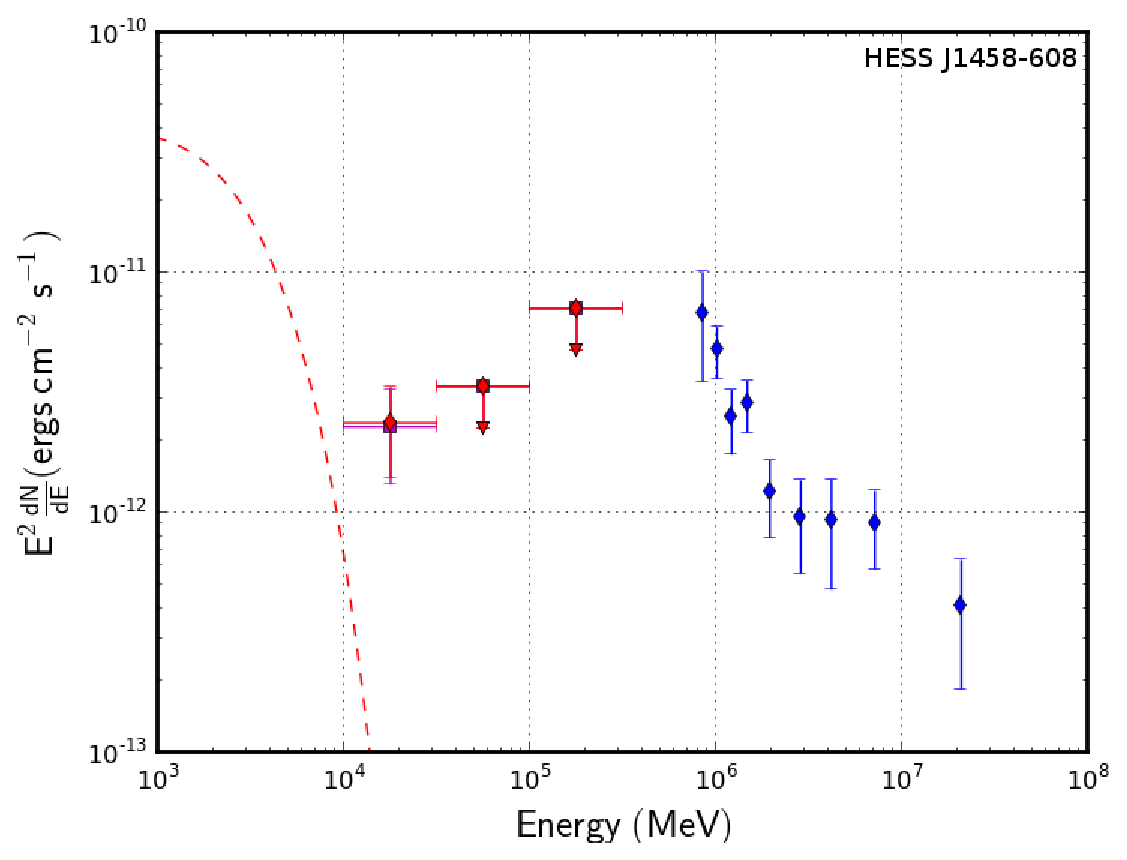
\includegraphics[width=0.60\textwidth]{figures/HESSJ1458.eps}
\caption{SED of HESS~J1458$-$608. H.E.S.S. spectral points are reported in blue while \emph{Fermi}-LAT spectral points are represented int red. The magenta points show the \emph{Fermi}-LAT points obtained once PSR~J1459$-$60 added to the model. The black error bars show the statistical and systematic uncertainties added in quadrature.
\label{fig:1458}}
\end{figure}

\begin{figure}[h!]
\centering
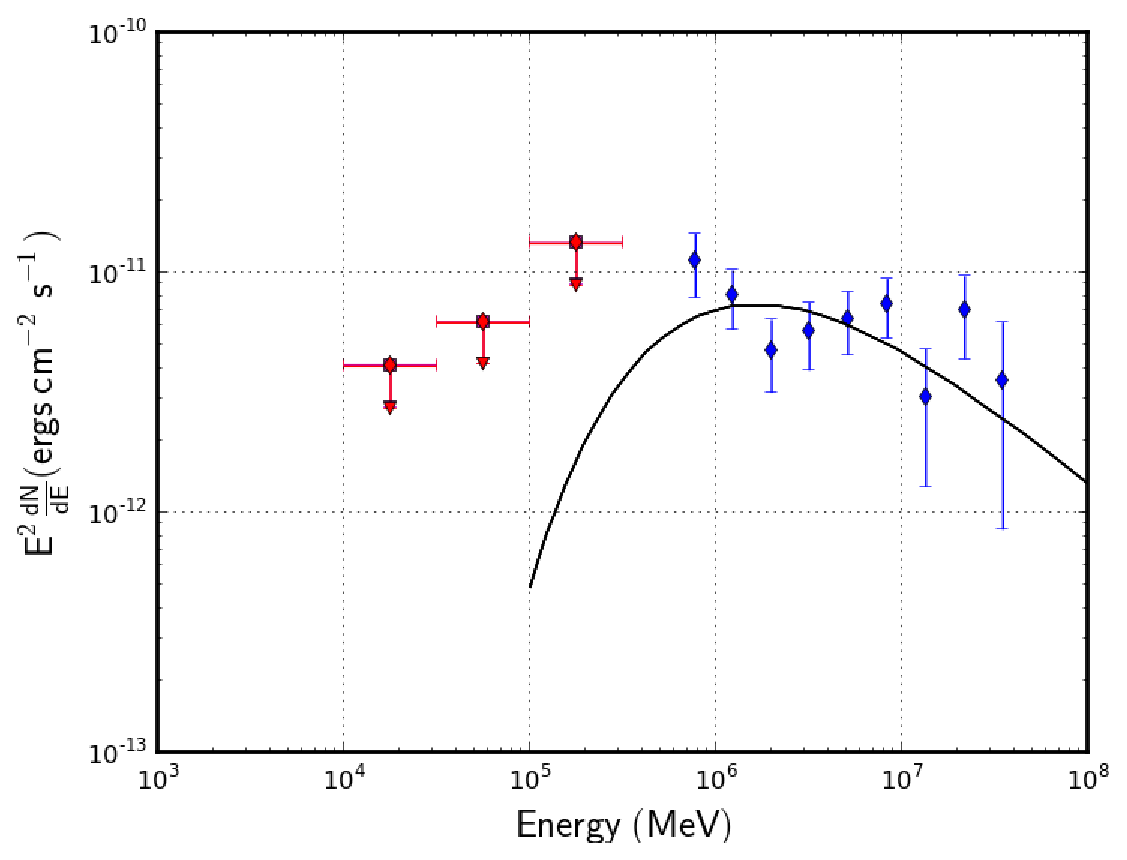
\includegraphics[width=0.60\textwidth]{figures/HESSJ1626.eps}
\caption{SED of HESS~J1626$-$490. H.E.S.S. spectral points are reported in blue while \emph{Fermi}-LAT upper-limits are indicated in red.
\label{fig:1626}}
\end{figure}

\begin{figure}[h!]
\centering
\subfigure{
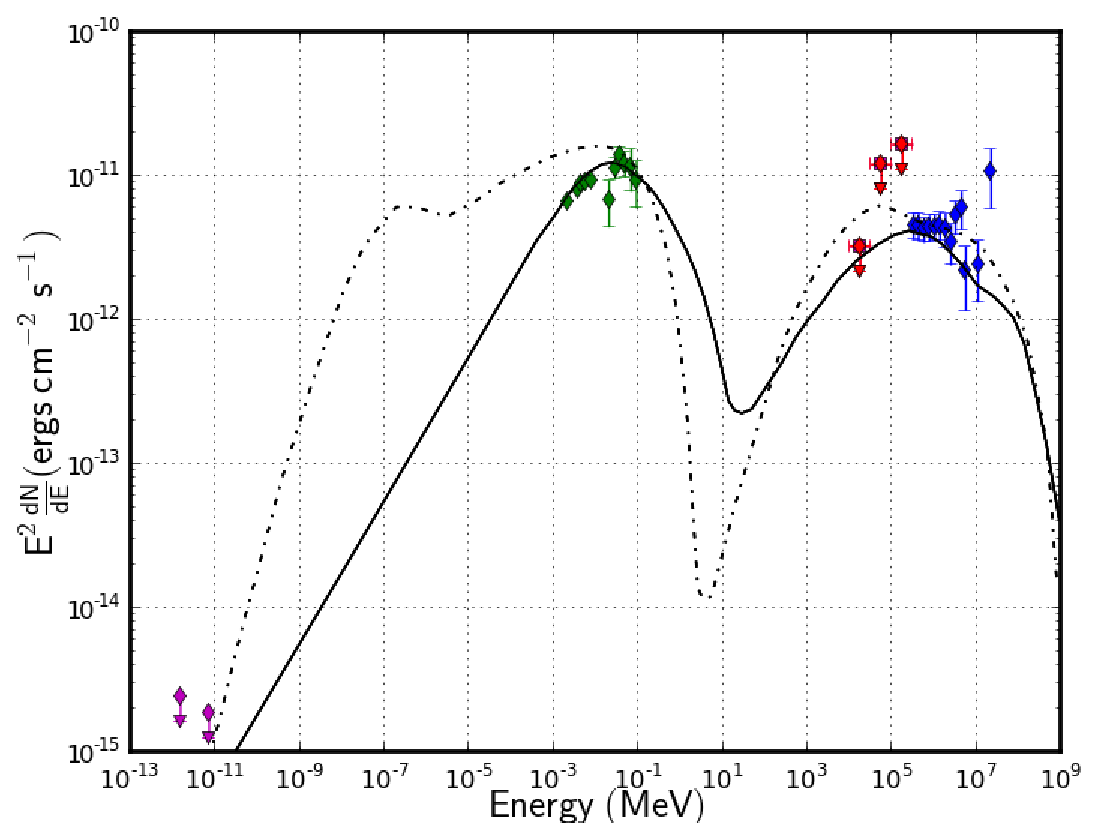
\includegraphics[width=0.60\textwidth]{figures/HESSJ1813178PWN.eps}}
\subfigure{
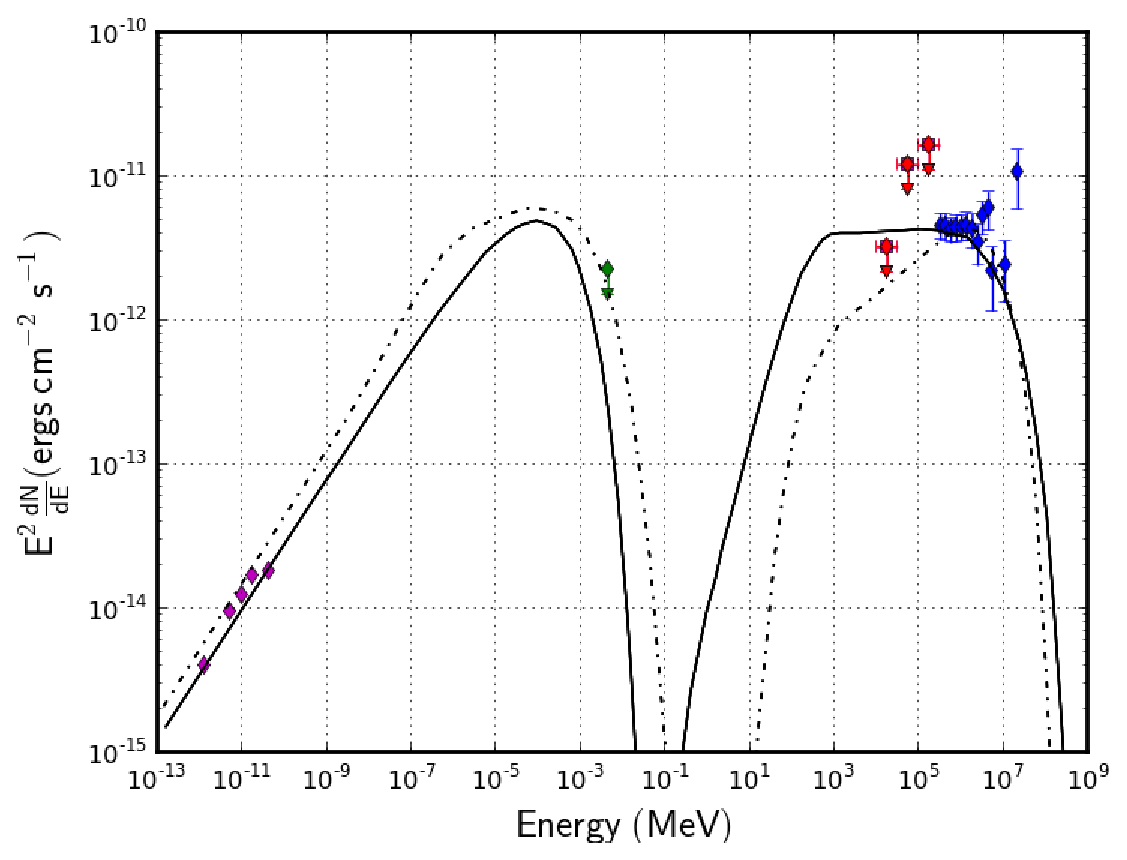
\includegraphics[width=0.60\textwidth]{figures/HESSJ1813178SNR.eps}}
\caption{SED of HESS J1813$-$178. The blue and red points show the H.E.S.S. \citep{2006ApJ...636..777A} and \emph{Fermi}-LAT spectral results. The radio data (magenta) are from VLA, Bonn, Parkes, and Nobeyama observatories \citep{2005ApJ...629L.105B}. The X-ray data are from XMM-Newton \citep{2007AA...470..249F}
and INTEGRAL \citep{2005ApJ...629L.109U}. These points were derived either for the shell of the SNR and for the core (PWN). The solid and dot dashed lines respectively correspond to the models proposed by \cite{2007AA...470..249F} and by \cite{2010ApJ...718..467F}. Top : Leptonic scenario in which the radiation is created by a PWN.  Bottom : Hadronic scenario in which the radiation is created by the SNR. 
\label{fig:hessj1813}}
\end{figure}




\clearpage

\begin{figure}[h!]
\centering
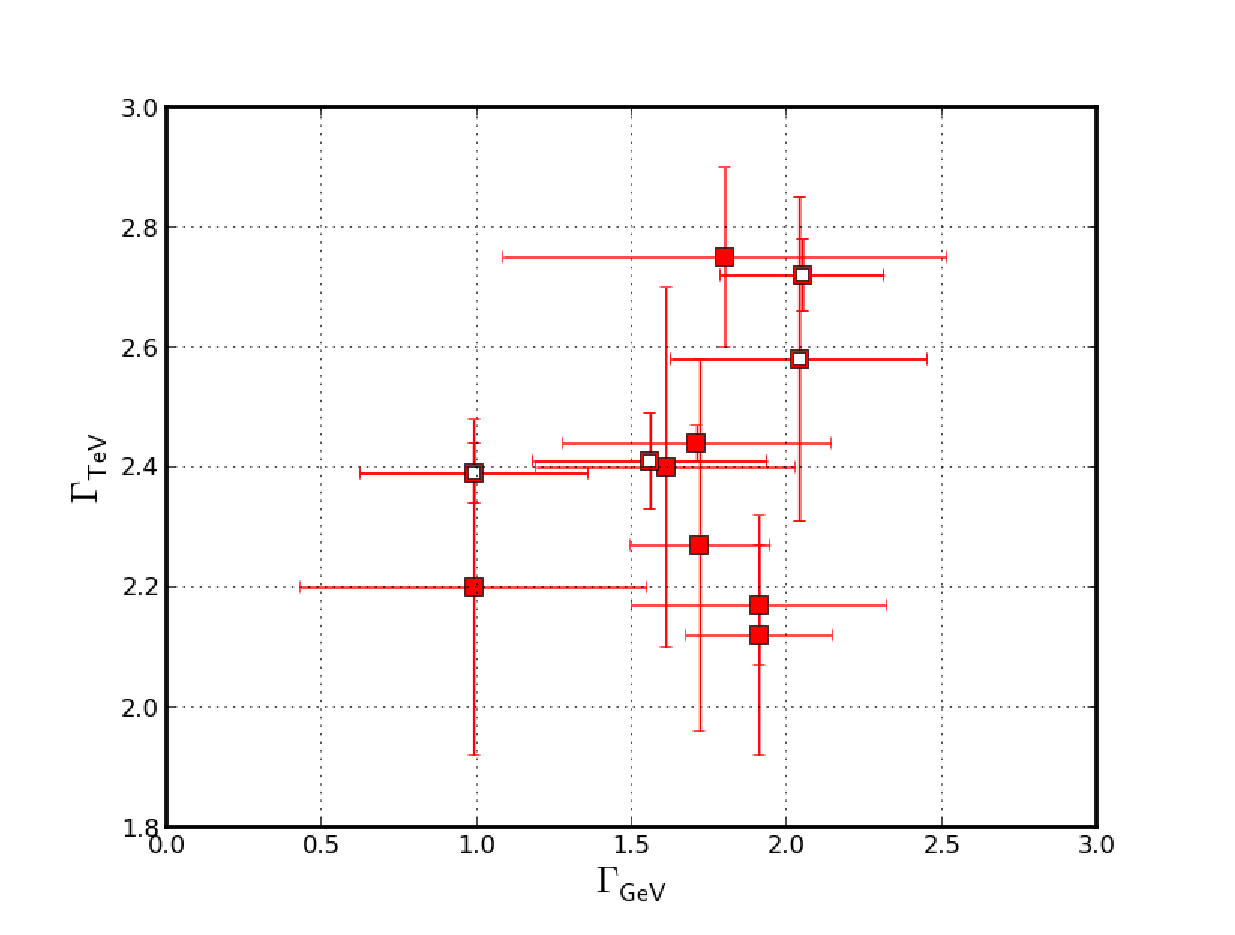
\includegraphics[width=0.5\textwidth]{figures/Gamma_GeV_Gamma_TeV.eps}
\caption{TeV spectral index as a function of the GeV spectral index for sources detected in our analysis for which the informations on the pulsar are available. These sources are summarized in Table \ref{tab:table_luminosity}. Full markers represent sources with a clear PWN association at TeV energies while hollow markers correspond to sources for which the association between TeV emission and a PWN is less clear. The dashed line corresponds to the symmetry compared to an index of 2. Pulsars summarized in Table \ref{tab:pulsarfit} are included in the model.
\label{fig:gammagamma}}
\end{figure}

\begin{figure}[h!]
\centering
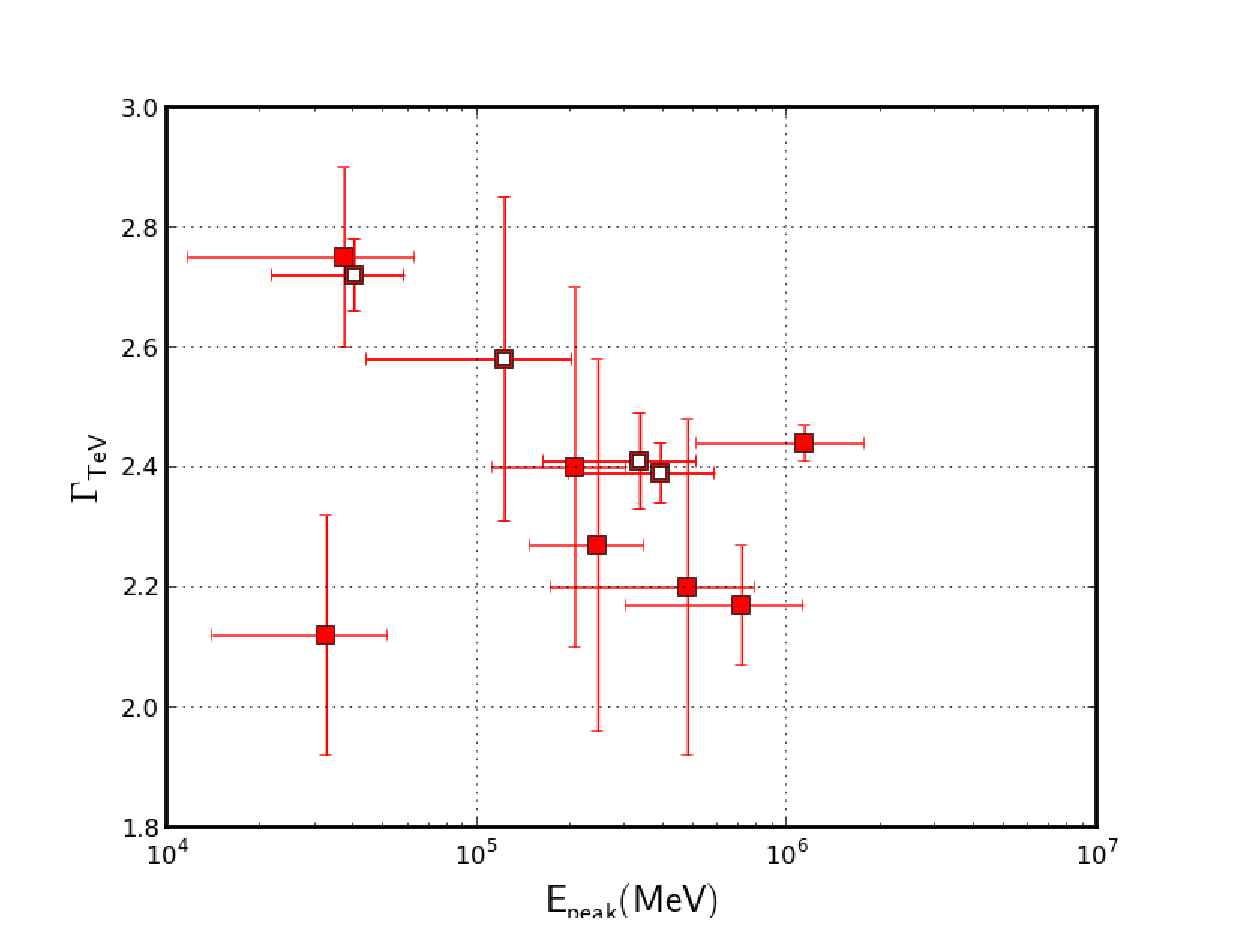
\includegraphics[width=0.5\textwidth]{figures/E_cut_vs_TeV.eps}
\caption{TeV spectral index as a function of the energy of the maximum of the IC peak for sources detected in our analysis for which the informations on the pulsar are available. These sources are summarized in Table \ref{tab:table_luminosity}. Full markers represent sources with a clear PWN association at TeV energies while hollow markers correspond to sources for which the association between TeV emission and a PWN is less clear. Pulsars summarized in Table \ref{tab:pulsarfit} are included in the model.
\label{fig:EpeakETeV}}
\end{figure}

\begin{figure}[h!]
\centering
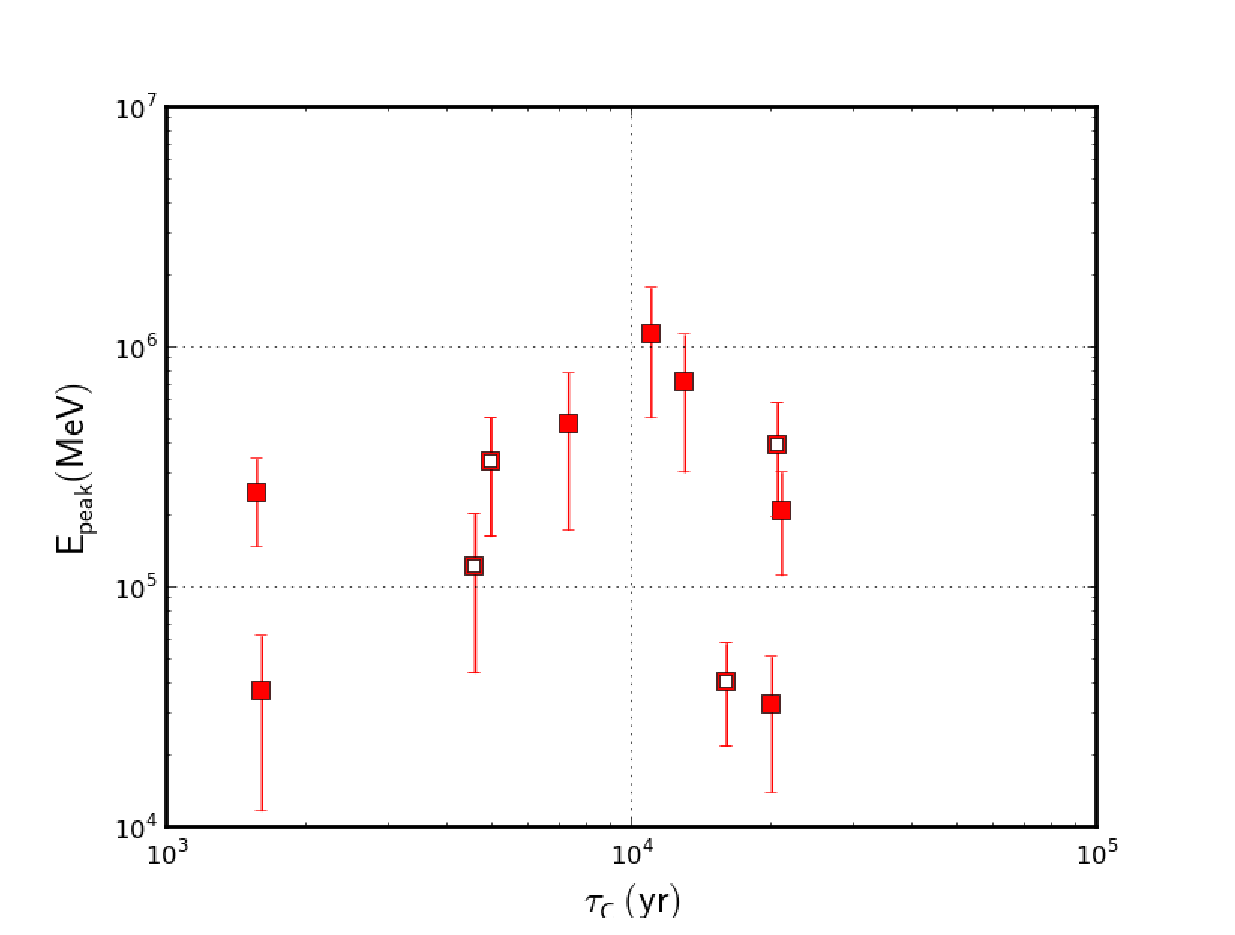
\includegraphics[width=0.5\textwidth]{figures/E_cut_vs_age.eps}
\caption{Energy of the maximum of IC peak as a function of the characteristic age of the pulsar for sources detected in our analysis for which the informations on the pulsar are available. These sources are summarized in Table \ref{tab:table_luminosity}. Full markers represent sources with a clear PWN association at TeV energies while hollow markers correspond to sources for which the association between TeV emission and a PWN is less clear. Pulsars summarized in Table \ref{tab:pulsarfit} are included in the model.
\label{fig:Epeakage}}
\end{figure}

\clearpage

\begin{figure}[h!]
\centering
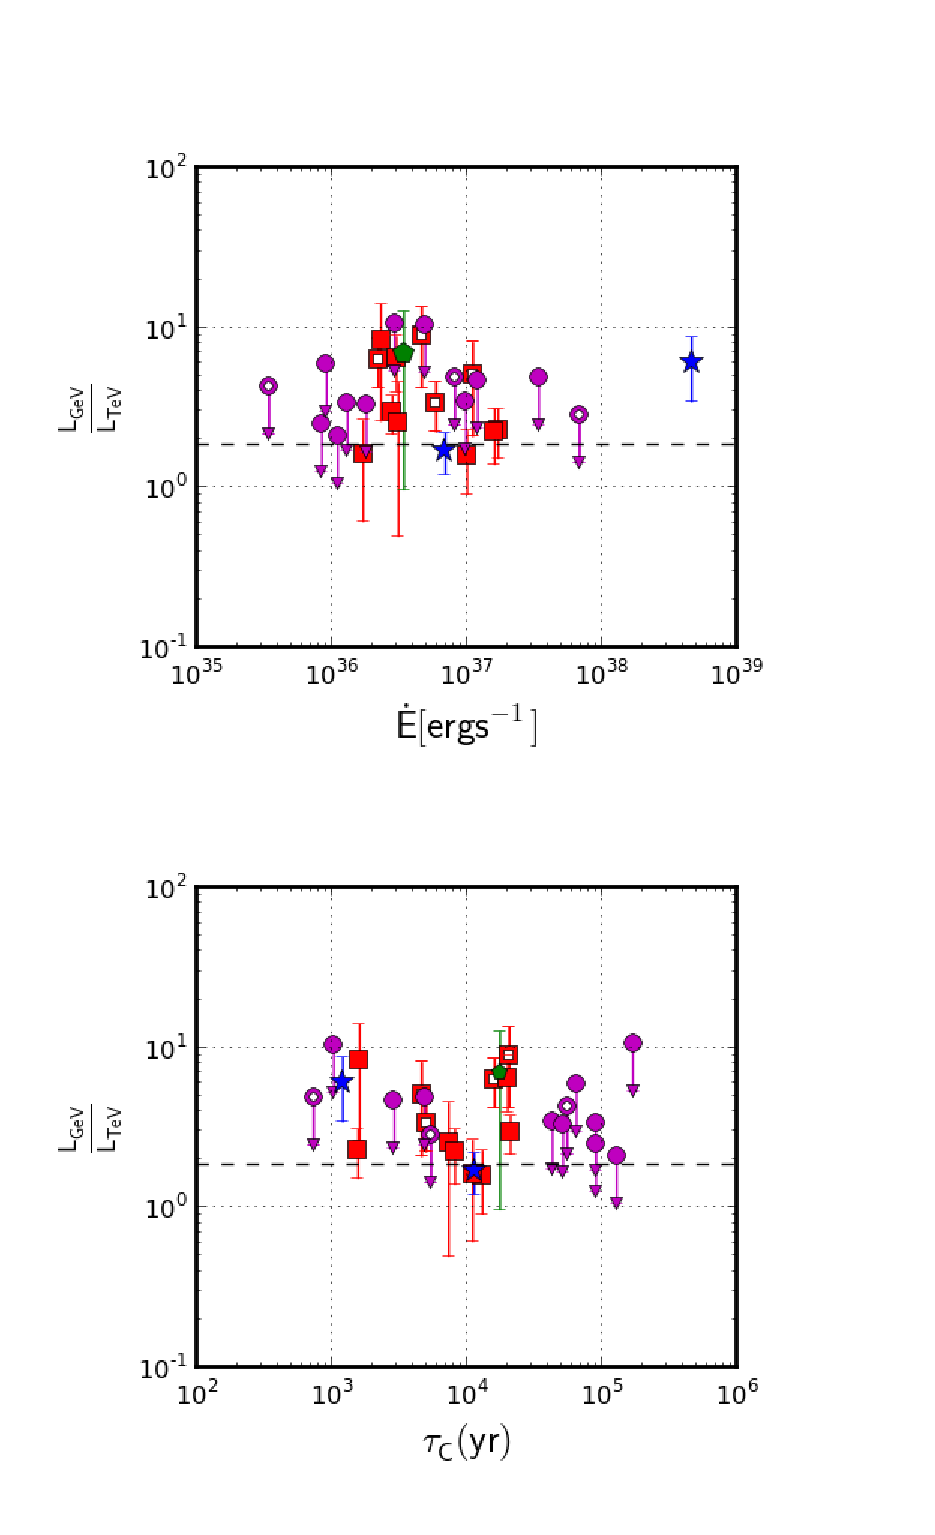
\includegraphics[width=0.5\textwidth]{figures/rapport_TeV.eps}
\caption{Ratio of luminosity of the PWN in GeV over the luminosity in TeV as a function of the pulsar spin-down power (top) and the pulsar characteristic age (bottom). Full markers correspond to sources with a clear PWN association at TeV energies while hollow markers correspond to sources for which the association between the TeV emission and a PWN is less clear. The red squares (\protect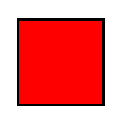
\includegraphics[scale=0.25]{figures/carrerouge.eps}) represent the sources detected at GeV energies, the magenta circles (\protect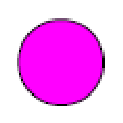
\includegraphics[scale=0.25]{figures/rondmagenta.eps}) show the upper limits, the green pentagon (\protect
\includegraphics[scale=0.25]{figures/pentagonevert.eps}) represent the sources showing a pulsar behaviour in the energy range and the blue stars (\protect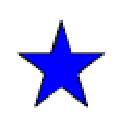
\includegraphics[scale=0.25]{figures/etoilebleue.eps}) represent the Crab nebula and Vela-X not studied in this work. Pulsars summarized in Table \ref{tab:pulsarfit} are included in the model. The dashed line represent the mean ratio found between the GeV and the TeV flux due to the spectral shape of the IC peak.
\label{fig:rapportTeV}}
\end{figure}

\clearpage

\begin{figure}[h!]
\centering
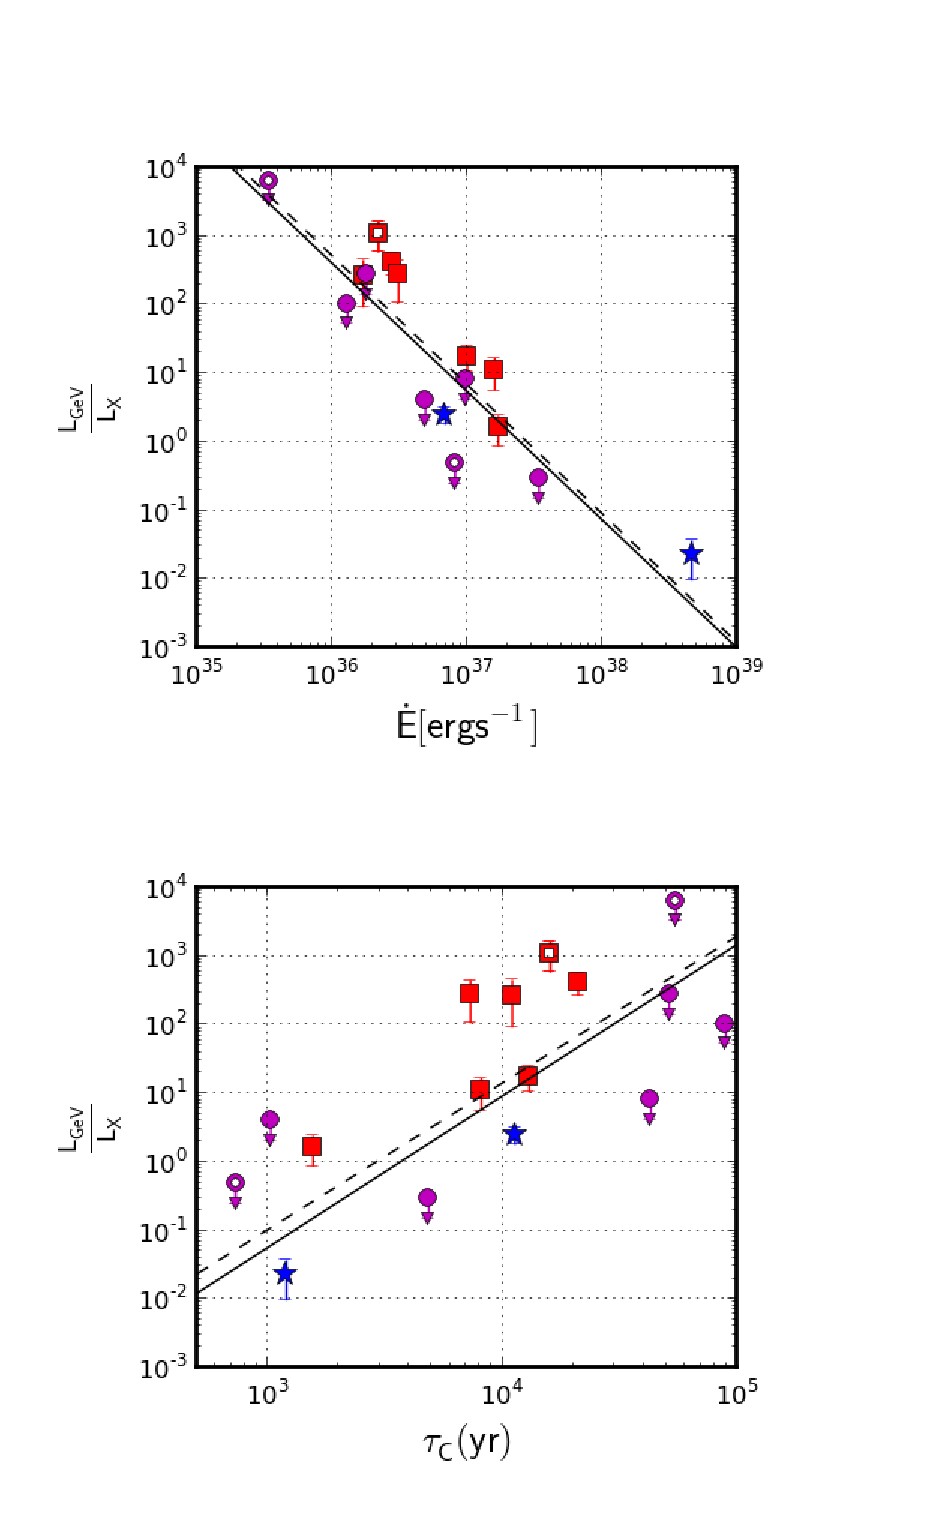
\includegraphics[width=0.5\textwidth]{figures/rapport_X.eps}
\caption{Ratio of luminosity of the PWN in GeV over the luminosity in X-rays as a function of the pulsar spin-down power (top) and the pulsar characteristic age (bottom). Full markers correspond to sources with a clear PWN association at TeV energies while hollow markers correspond to sources for which the association between the TeV emission and a PWN is less clear. The red squares (\protect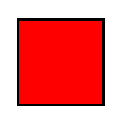
\includegraphics[scale=0.25]{figures/carrerouge.eps}) represent the sources detected at GeV energies, the magenta circles (\protect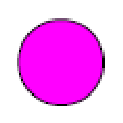
\includegraphics[scale=0.25]{figures/rondmagenta.eps}) show the upper limits, the green pentagon (\protect
\includegraphics[scale=0.25]{figures/pentagonevert.eps}) represent the sources showing a pulsar behaviour in the energy range and the blue stars (\protect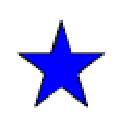
\includegraphics[scale=0.25]{figures/etoilebleue.eps}) represent the Crab nebula and Vela-X not studied in this work. Pulsars summarized in Table \ref{tab:pulsarfit} are included in the model. The dashed and solid lines represent respectively the relations derived in \cite{2009ApJ...694...12M} multiplied by $\bar{R}$ for the whole sample of sources and for the sources clearly identify to PWNe.
\label{fig:rapportX}}
\end{figure}

\clearpage

\begin{figure}[h!]
\centering
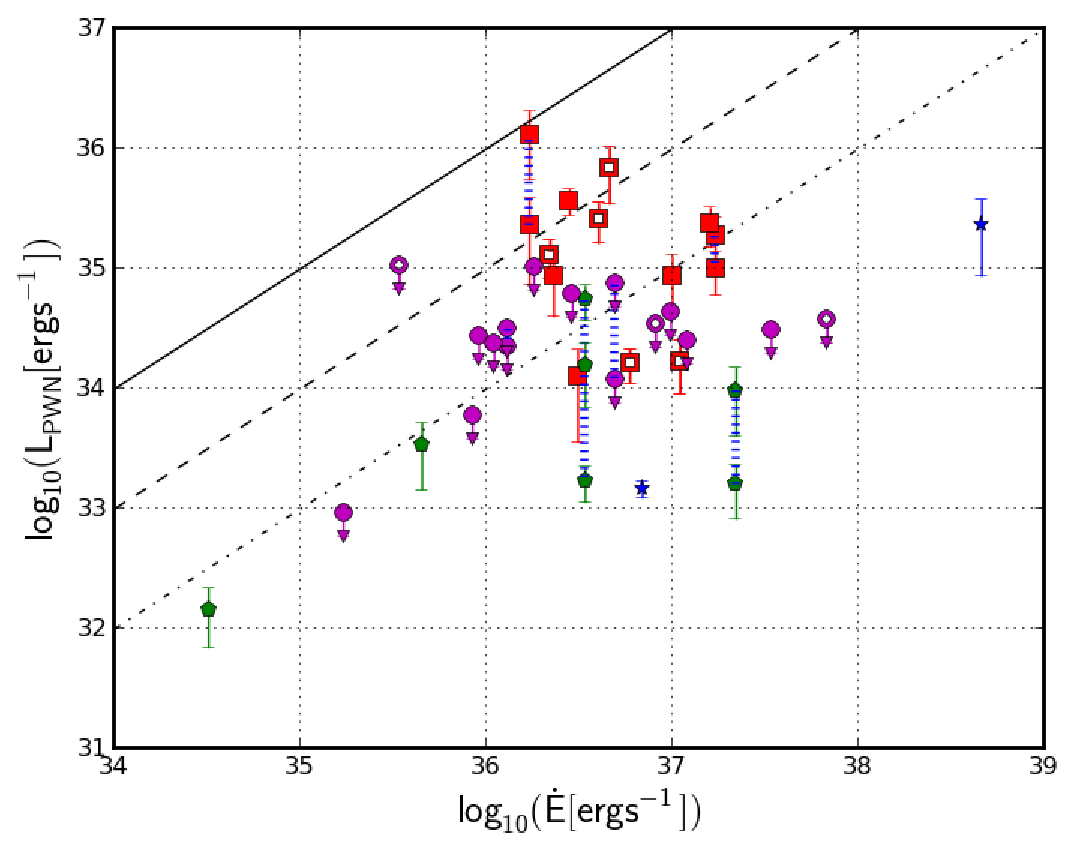
\includegraphics[]{figures/dotelpwn.eps}
\caption{Luminosity of the PWN as a function of the pulsar spin-down power. Full markers correspond to sources with a clear PWN association at TeV energies while hollow markers correspond to sources for which the association between the TeV emission and a PWN is less clear. The red squares (\protect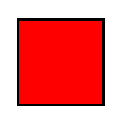
\includegraphics[scale=0.25]{figures/carrerouge.eps}) represent the sources detected at GeV energies, the magenta circles (\protect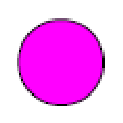
\includegraphics[scale=0.25]{figures/rondmagenta.eps}) show the upper limits, the green pentagon (\protect
\includegraphics[scale=0.25]{figures/pentagonevert.eps}) represent the sources showing a pulsar behaviour in the energy range and the blue stars (\protect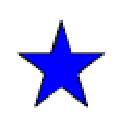
\includegraphics[scale=0.25]{figures/etoilebleue.eps}) represent the Crab nebula and Vela-X not studied in this work. Sources with two distances estimates have two markers connected with a dotted blue line. Pulsars summarized in Table \ref{tab:pulsarfit} are included in the model. 
\label{fig:dotelpwn}}
\end{figure}

\clearpage


\clearpage
\appendix
\renewcommand{\thefigure}{A-\arabic{figure}}
\setcounter{figure}{0}
\appendix


\end{document}
